% LyX 2.2.3 created this file.  For more info, see http://www.lyx.org/.
%% Do not edit unless you really know what you are doing.
\documentclass[english]{article}
\usepackage{lmodern}
\usepackage[T1]{fontenc}
\usepackage[latin9]{inputenc}
\usepackage[letterpaper]{geometry}
\geometry{verbose,tmargin=1.25in,bmargin=1.25in,lmargin=1.25in,rmargin=1.25in}
\usepackage{babel}

\usepackage[labelsep=period]{caption}
\renewcommand{\thetable}{\Roman{table}}


\usepackage{enumitem}
\usepackage{float}
\usepackage{rotfloat}
\usepackage{makecell}
\usepackage{units}
\usepackage{amsmath}
\usepackage{amssymb}
\usepackage{bbm}
\usepackage{graphicx}
\usepackage{grffile}
\usepackage{setspace}
\usepackage[dvipsnames]{xcolor}
\usepackage[authoryear]{natbib}
\doublespacing
\usepackage[unicode=true]{hyperref}
\usepackage{verbatim}

\usepackage{setspace}


% table of contents within appendix
\usepackage{appendix}
\usepackage{titletoc}
\newcommand\DoToC{%
	\startcontents
	\printcontents{}{2}{\textbf{Contents}\vskip3pt\hrule\vskip5pt}
	\vskip3pt\hrule\vskip5pt
}


\onehalfspacing            

 
 \newenvironment{myenum}
{ \begin{enumerate}
    \setlength{\itemsep}{0pt}
    \setlength{\parskip}{0pt}
    \setlength{\parsep}{0pt}     }
{ \end{enumerate}      } 

\makeatletter

% Keywords command
\providecommand{\keywords}[1]
{
  \small	
  \textbf{\textit{Keywords---}} #1
}

%%%%%%%%%%%%%%%%%%%%%%%%%%%%%% LyX specific LaTeX commands.
%% Because html converters don't know tabularnewline
\providecommand{\tabularnewline}{\\}

%%%%%%%%%%%%%%%%%%%%%%%%%%%%%% Textclass specific LaTeX commands.
\providecommand*{\code}[1]{\texttt{#1}}

%%%%%%%%%%%%%%%%%%%%%%%%%%%%%% User specified LaTeX commands.
\usepackage{booktabs}
\usepackage{pdflscape}
\usepackage{pbox}
\usepackage{multirow}
\usepackage{makecell}
\usepackage{graphicx}
\usepackage{array}
\usepackage{amsmath, amsthm, amssymb}
\usepackage{mathtools}
\usepackage{dsfont}
\newcommand*\ExpandableInput[1]{\@@input#1 }
\setlength{\footnotesep}{12pt}
\DeclareMathOperator{\E}{E}

\newtheorem{prop}{Proposition}
\newtheorem{conj}{Conjecture}
\newtheorem{lemma}{Lemma}
\newtheorem{cor}{Corrolary}
\theoremstyle{definition}
\newtheorem{exmp}{Example}

\DeclareMathOperator*{\argmax}{arg\,max}

\makeatother

\begin{document}

	
\begin{singlespace}

\title{\vspace*{-1cm}Peak-Hour Road Congestion Pricing: \\ Experimental Evidence and Equilibrium Implications
\thanks{I am deeply grateful to Ben Olken, Esther Duflo, Frank Schilbach, and Edward Glaeser for support throughout this project. I am indebted to Matt Turner for his discussion of the paper. I thank Alex Bartik, Nikhil Agarwal, Moshe Ben-Akiva, Peter Christiansen, Vikas Dimble, Benjamin Faber, John Firth, Andrew Foster, Chishio Furukawa, Nick Hagerty, Rachel Glennerster, Tetsuya Kaji, Myrto Kaloupsidi, Jing Li, Matt Lowe, Leslie Martin, Rachael Meager, Yuhei Miyauchi, Scott Nelson, Will Rafey, Otis Reid, Mahvish Shaukat, and Dan Waldinger for many helpful suggestions. Anupriya Khemka, Keerthana Jagadeesh, and Ashwin MB provided excellent research assistance. I also thank Mohannad Abunassar, Maryam Archie, Priya Chetri, Sasha Fleischman, Mahima Gupta, Aditi Sinha, Mamta Jat, Kristina Kelhofer, Michelle Nenciu, Sebastian Quinones, Sarvottam Salvi, Meghna Singh, Sahana Subramanyam, Tammy Tseng, Thuy Duong Vuong, Lantian Xiang, and Massieh Zare, who contributed valuable research assistance at various stages of the project. I gratefully acknowledge design and technical support for the smartphone app ``Bangalore Traffic Research'' from Adrian Drewett and Dharmendra Singh from Gridlocate Ltd. Funding for this project was generously provided by the Weiss Family Fund for Research in Development Economics, the IGC Cities Fund, the J-PAL Pilot Fund, and the J-PAL Urban Services Initiative Pilot Fund. This project has human subjects approval from MIT COUHES (protocol 1511312369A002), IFMR (IRB00007107), Harvard CUHS (IRB19-0456) and was registered in the AEA RCT Registry (AEARCTR-0002083).

%Online Appendix available at \protect\url{sites.google.com/site/gabrielkreindler/cp-sm}. 
}}
\end{singlespace}
\begin{singlespace}

\author{Gabriel E. Kreindler\thanks{Department of Economics, Harvard University. Email: \texttt{gkreindler@fas.harvard.edu}.}}
\end{singlespace}
\begin{singlespace}

\date{\today \vspace*{-1cm}}
\end{singlespace}
\maketitle


\begin{abstract}

Developing country megacities suffer from severe road traffic congestion, yet the level of congestion is not a direct measure of equilibrium inefficiency. I study the peak-hour traffic congestion equilibrium in Bangalore. To measure travel preferences, I use a model of departure time choice to design a field experiment with congestion pricing policies and implement it using precise GPS data. Commuter responses in the experiment reveal moderate schedule inflexibility and a high value of time. I then show that in Bangalore, traffic density has a moderate and linear impact on travel delay. My policy simulations with endogenous congestion indicate that optimal congestion charges would lead to a small reduction in travel times, and small commuter welfare gains. This result is driven primarily by the shape of the congestion externality. Overall, these results suggest limited commuter welfare benefits from peak-spreading traffic policies in cities like Bangalore.

\end{abstract}

\newpage{}

\section{Introduction}

Traffic congestion is a significant and pervasive problem in large cities, especially in developing countries, where the urban population and private vehicle ownership are growing rapidly. For example, the fastest large city in India is slower than the slowest large city in the US \citep{akbar2018}. Long and unreliable travel times reduce the agglomeration benefits of large cities, whether for accessing jobs, markets, services or amenities.

Commuters who drive in congested conditions impose externalities by increasing travel times for the other commuters on the road. Since congestion is higher during rush hour, peak-hour traffic jams may be particularly inefficient. Reflecting this concern, several urban road traffic policies focus on reducing peak-hour congestion, either through pricing or quantity restrictions.\footnote{The congestion charge policy in Stockholm and Singapore's Electronic Road Pricing (ERP) policy have higher fees during the morning and evening peak hours. Jakarta's former ``3-in-1'' and the current ``odd-even'' policies are in effect during morning and evening peak hours only. Similarly, Manila's Unified Vehicular Volume Reduction Program (UVVRP) only applies during peak hours in certain parts of the city.} 

However, while congestion pricing is the textbook policy response to traffic externalities, its quantitative relevance to traffic congestion in developing countries is an empirical question. The deadweight loss due to peak-hour congestion depends on how commuters substitute across departure times, and on the magnitude of the externality and how it differs across departure times.

In this paper, I study the  impact of peak-hour congestion pricing on driver behavior and on the peak-hour traffic congestion equilibrium in Bangalore, India. I measure the following demand and supply fundamentals that I will hold fixed in counterfactuals. First, I estimate commuter substitution patterns across departure times, given by schedule costs and desired arrival times, using precise data on urban travel behavior and experimental price variation. Second, I use within-day variation to estimate the causal effect of traffic density on travel speed, thereby characterizing the road traffic externality in Bangalore given the current road network, vehicle composition and driving styles.

% Model
I set up an equilibrium model of peak-hour congestion based on the classic trip scheduling model \citep{vickrey1969}. In my model, commuters face a distribution of travel times for each departure time and choose an optimal trip departure time. (For model estimation, I also incorporate a dynamic choice between two routes that differ in travel time profiles.) The key preference parameters are the schedule costs of arriving early or late relative to an ideal arrival time, and the value of travel time (VOTT). Commuters have rich heterogeneity given by an unobserved distribution of ideal arrival times and logit or nested logit shocks. 
This heterogeneity covers a wide range of substitution patterns over departure times. This ranges from highly elastic decisions when commuters share the same ideal arrival time and logit and travel time uncertainty vanish, as in \citet{Arnott1993}, to the case where each commuter is highly inflexible around their ideal arrival times, and ideal arrival times vary across commuters and days. To close off the model, the profile of congestion is determined endogenously by aggregate departure rates. I also analyze an equilibrium model extension with two routes that have different externalities (as in \citealt{walters61}), and another extension with an extensive margin decision.

I use a version of this model to design a field experiment with congestion charge policies to estimate the preference parameters. I implement the experiment within a sample of 497 commuters in Bangalore. I collected detailed travel behavior data using a smartphone app that passively logged GPS location data from study participants. The two congestion pricing policies induce exogenous cost variation along the departure time and travel time dimensions. The ``peak-hour'' pricing policy gives some commuters marginal incentives to change their departure times. Under the ``route'' pricing policy, commuters pay a flat fee for driving through a circular area located along their usual route. The area is chosen individually for each commuter to induce a choice between a quick, expensive route and a longer free detour route. I implement the experiment using a smartphone app and a pre-paid account. To focus on intensive margin responses and to prevent gaming, participants were charged on days when they did not make any trips. Intuitively, commuter departure time and route choices with and without these two pricing policies help identify the departure time substitution patterns (given by schedule costs and the distribution of ideal arrival times) and VOTT.

% reduced form results - DT
Commuters respond to the two treatments by changing departure times and routes to avoid charges. Under ``peak-hour'' charges, in the morning before the peak-hour, commuters left around 3--4 minutes earlier on average, with an imprecise response after the peak-hour. My results for the evening peak-hour are less precise, but consistent with commuters leaving later after the peak. 
Under ``route'' charges, participants use the detour (free) route 27 percentage points more often. Higher detour route usage persists after charges end, including among commuters who used a detour route before the experiment.
I find no impact on the number of trips for either treatment.\footnote{As participants were charged on days when they did not make any trips, this should not be interpreted as the extensive margin response to charges.}

% structural
I use moments that exploit the experimental price variation to estimate the travel demand model of departure time and route choice for the morning commute. 

% results VOTT
The estimated value of travel time is 611 INR per hour (9.5 USD at market exchange rates or 29.6 USD PPP in 2017). This is significantly larger than the average self-reported hourly wage in this sample, indicating that commuters significantly dislike driving in Bangalore. VOTT is identified separately from a route switching cost included in the dynamic route choice model. Another reason for large estimated VOTT is that my results are relative to time differences based on Google Maps, while commuters in this sample overestimate differences in travel times.

% schedule flexibility
The estimated schedule costs of early and late arrival are 545 INR per hour and 3448 INR per hour, showing that commuters are relatively schedule inflexible. The cost of early arrival is 89\% of VOTT, higher than previous estimates \citep{small1982}. As a benchmark, this ratio would be 15\% for the median-length home to work trip in my sample if the steepest part of the travel time profile in Bangalore reflected compensating differentials for schedule costs versus travel time. The cost of late arrival to VOTT that I find is smaller than previous estimates.


%%% MEASURE EXTERNALITY
On the supply side, I next measure the road traffic externality. To measure traffic density, I use around 140,000 GPS trips collected using the smartphone app over six months in 2017. I use Google Maps data to measure instantaneous travel delay (inverse speed). To identify the causal impact of traffic density on travel delay, I use hour-of-day instruments that capture large shifts in demand, including between peak- and off-peak-hours.

Citywide traffic density has a moderate and linear impact on travel delay. The linear relationship is robust for all calendar dates and when zooming in to major arteries. I find no evidence of convexity for high levels of traffic. Quantitatively, a 7 km long peak-hour trip increases total driving time in Bangalore by approximately 15 minutes. I discuss the validity of the instruments and additional robustness results. The citywide relationship that I estimate is biased if commuters substitute to higher-externality roads during the peak-hour \citep{walters61}. I use Google Maps route data to show that this effect is small for Bangalore commuters.

%% Part 5
In the final part of the paper, I simulate an equilibrium model where commuters decide when to travel, and congestion is determined endogenously. Commuters are endowed with the preferences I estimate from my field experiment, and congestion is determined by the road network technology I estimate from GPS data. In the benchmark model, commuters have a single route. I compare the unpriced Nash equilibrium to the social optimum implemented with equilibrium optimal departure time by trip length Pigouvian congestion charges, assuming zero policy implementation costs and lump-sum revenue redistribution.

Through the lens of the model, optimal departure time charges have a small effect on commuter welfare. Under the social optimum, peak congestion is lower and the average trip duration goes from 37.3 to 34.8 minutes on average, a $17.1\%$ reduction in average travel time above free-flow. Commuter welfare---which also includes schedule costs---increases by 8.9 INR (43 US cents PPP). The deadweight loss due to peak-hour congestion is $2.2\%$, or $5.7\%$ as a share of commuter costs excluding free-flow costs. As a benchmark, the latter figure is 50\% in the bottleneck model from \citet{Arnott1993}, where commuters are perfectly elastic across departure times.

Why is the deadweight loss due to peak-hour congestion so low in Bangalore? In a standard model with a negative consumption externality over one good, deadweight loss is given by the Harberger triangle, whose area is increasing in the marginal external cost and in the demand elasticity. In my model, each departure time imposes a different externality. Commuters have very ``local'' substitution patterns over departure times, and the linear estimated road technology implies that the marginal external cost of travel is very similar for nearby departure times. These two facts imply that there is little room for efficiency gains by changing when commuters travel.

Deadweight loss depends significantly on the road technology. Welfare gains of optimal pricing are almost five times larger if I assume that travel density is a power of traffic volume with exponent $1.5$. Since the shape of the road traffic externality may be different in other cities, measuring city-wide road traffic externalities is of first-order importance. The welfare gain is higher in an equilibrium model where commuters choose between two routes with different externalities \citep{walters61}.

Preferences also matter, although to a lesser extent. Holding the observed distribution of departure times approximately fixed, if early schedule costs were four times smaller, welfare gains from optimal pricing would be 3.6\% (63\% higher than in the baseline model). Adding preference heterogeneity proportional to wages has a similar effect.

My simulations ignore longer-term margins of adjustment, such as commuter and firm location choices \citep{tsivanidis2019, herzog22}. Congestion pricing can have ambiguous effects on welfare in such contexts \citep{brinkman20161}. To provide some insight into other margins of behavior, I run simulations where commuters can adjust along the extensive margin, a catch-all for using travel modes with negligible externalities (such as public transportation) and for canceling trips. Welfare gains remain low for reasonable values of the elasticity of trips with respect to total trip cost.



\section{Related Literature\label{sec:lit}}
This paper builds on an extensive theoretical literature analyzing optimal and second-best pricing with peak-hour road traffic congestion \citep{vickrey1969, small1982, Arnott1993, noland1995travel, hall2018, hall2019}. My model builds on the canonical trip scheduling model, adding and estimating additional sources of heterogeneity to better match individual travel behavior data.

The dynamic model of traffic congestion I use here is related to the hydrodynamic or kinematic model with the assumption of instantaneous propagation of traffic density in the entire city \citep{mahamassani84, small2007}. Other canonical models of peak-hour congestion are the bottleneck model with fixed capacity \citep{vickrey1969, Arnott1993}, and models without propagation \citep{chu1995, henderson1974}. My approach to instrument for traffic density using hour-of-day (demand) instruments is similar to \citet{duranton2017}, \citet{hughes18}, and \citet{anderson2020}.

The approach in this paper to design an experiment based on the model brings together two previous literatures. First, some papers use discrete choice models to estimate the value of time, of reliability, or of urgency from real-world driver decisions to use a faster tolled lane \citep{small2005, bento2017}. A separate group of papers analyzes reduced form impacts of road pricing experiments \citep{tillema2013, martin2017, hintermann22}. Here, the randomized experiment is designed to transparently recover the key commuter preference parameters in the model.

A related empirical literature documents the impact of real-world traffic policies on traffic volumes, travel times and air pollution, either for the aggregate impact of  congestion pricing policies in London, Stockholm and Milan \citep{tfl2006,prudhomme2005,roux2005,gibson2015,karlstrom2009}, or for non-price, vehicle quantity restrictions in developing countries \citep{davis2008, kreindler-2016, Hanna89, gu2017}.

\citet{duranton2017} reach a similar conclusion of low deadweight loss due to traffic congestion for Bogot\'a, Colombia, using a representative household travel survey and Google Maps travel time data to estimate the demand for trips and supply of travel by time of day. My paper's key contributions are to explicitly incorporate substitution between different times of the day in the equilibrium model, and using an experiment to estimate demand.



\section{Traffic Congestion and Travel Behavior in Bangalore, India\label{sec:Setting}}

Similar to other large cities in developing countries, Bangalore's fast growth put stress on its transportation network. \citet{akbar2018} rank Bangalore as the most congested city in India. 

Figure \ref{fig:Average-Predicted-Travel} shows travel delay based on travel times collected using the Google Maps API. On average between 7 am and 10 pm on weekdays and across all routes, it takes 3.6 minutes to advance one kilometer (10.3 miles per hour). This is extremely slow, in line with speeds in other large cities in developing countries \citep{Hanna89, kreindler-2016}. 

Figure \ref{fig:Average-Predicted-Travel} also shows strong predictable within day variation in traffic congestion. Between 7 am and 9 am, travel delay increases by 1.38 minutes per kilometer. A trip that would take $40$ minutes starting at 7 am would take more than an hour starting at 9 am. Most of the day to day variation in traffic in Bangalore is explained by route-by-departure time cells.

These patterns suggest that commuters exert high externalities during the peak-hour, and that a more efficient allocation might involve some of them leaving earlier or later. Individual-level travel behavior data from GPS data (discussed in section \ref{sec:GPS-Data}) is consistent with high schedule flexibility. Most commuters vary their departure times significantly from day to day. For the median person, the standard deviation of the departure time for the first trip of the day from home to work is 29 minutes, which implies a 95\% probability interval of almost two hours (Table \ref{tab:Descriptive-Statistics-about}, panel C). However, this daily variation does not automatically imply that commuters are schedule flexible. It is possible that desired travel times change from day to day (based on changes in work or other constraints) and commuters are inflexible around those times on any particular day. The model and experiment will help clarify and quantify these issues.

Separately, the peak-hour congestion profile is not directly informative about the magnitude of the traffic externality, which also depends on the underlying variation in traffic density.

\section{Theoretical Framework\label{sec:Theoretical-Framework}}
\label{sec:model}
I set up an equilibrium model of peak-hour traffic congestion where commuters choose optimal departure times based on the profile of traffic congestion and ideal arrival times. To study experimental variation in travel time, I extend the model to include route choice in a dynamic setting. I discuss how the elasticities identified in partial-equilibrium pricing experiments relate to the key travel demand model parameters. On the supply side, the congestion profile is endogenous, given by a dynamic model where instantaneous speed depends on traffic density. 

\subsection{Travel Demand: Departure Time Choice \label{subsec:dep-time-model}}

A mass of atomistic commuters $i$ decide when to travel from home to work on day $t$. The decision to make a trip is inelastic. (I add an extensive margin decision in section \ref{sec:Policy-Counterfactual-Simulation}.) 

To begin, consider the case with a single route. Departure time $h$ takes discrete values, for example every minute. Utility at departure time $h$ depends on realized travel time $T$ and ideal arrival time $h^A$ as
\begin{equation*}
	\label{eq:utility-common}
	v(h,T,h^A) = -\alpha T -\beta_{E}\left|h + T - h^A\right|_{-} - \beta_{L}\left|h + T - h^A\right|_{+}.
\end{equation*}
Travel time cost is linear and $\alpha$ measures the marginal value of travel time (VOTT). The second and third terms are the canonical way to measure scheduling preferences over arrival time $h + T$ \citep{Arnott1993}. Schedule heterogeneity is defined by an ideal arrival time $h^A$, and schedule costs by constant per-unit of time costs of arriving early $\beta_{E}$ and of arriving late $\beta_{L}$.\footnote{$\left|x\right|_{-}$ and $\left|x\right|_{+}$ denote the negative and positive parts of $x$.} 

Travel time $T_{it}(h)\sim \mathcal T_{i}(h)$ is random and realized after departure, drawn i.i.d. over days $t$. I assume that the researcher observes the distributions $\mathcal{T}_i(h)$. For any travel time distribution $\mathcal T$, I denote expected utility
\begin{equation}
	\label{eq:utility-common-expected}
	\mathbb{E} v(h,\mathcal T,h^A) = \mathbb{E}_{T\sim \mathcal T}\ v(h,T,h^A).
\end{equation}

This model captures the main forces that determine departure time decisions within the peak-hour equilibrium, and it makes several parametric assumptions. Travel time costs are linear, and schedule costs are piece-wise linear. However, uncertainty in travel time smooths out the profile of schedule costs, and makes it more difficult to arrive close to the ideal arrival time. This implicitly generates a value of travel time reliability. In the benchmark model, the parameters $\alpha$, $\beta_E$, $\beta_L$ are the same for all commuters. I later estimate a model where these parameters scale with income.

Each morning, the commuter observes the ideal arrival time $h_{it}^A$, idiosyncratic shocks $(\varepsilon_{it}(h))$, and monetary charges $p_{it}(h)$, and chooses departure time to maximize expected utility,
\begin{equation}
	\label{eq:utility-1-route}
	u_{it}(h,h_{it}^A)=\mathbb{E}v(h,\mathcal T_{i}(h), h_{it}^A) - p_{it}(h) + \varepsilon_{it}(h).
\end{equation}
The idiosyncratic shocks $\varepsilon_{it}(h)$ are distributed according to a type-1 extreme value distribution with scale $\sigma^{DT}$, and they capture daily factors that affect departure times, such as waking up earlier or having to complete an unexpected task before leaving. This leads to multinomial logit choice probabilities conditional on $h_{it}^A$.

The ideal arrival time is a second source of individual heterogeneity in the model. As explained below, this allows for more flexible substitution patterns between departure times. The ideal arrival time $h_{it}^A$ is drawn i.i.d. over days $t$ from an individual-specific distribution over a discrete grid, with probability density function $f_i^A$. The researcher does not observe $f_i^A$. This distribution is not affected by pricing experiments, and I hold it fixed in counterfactuals. The distribution of ideal arrival times is individual-specific to help account for the variation of departure times both across and within commuters in the data (Table \ref{tab:Descriptive-Statistics-about}). 

\paragraph{Model Identification.} The goal of demand estimation in this setting is to separately identify the value of travel time ($\alpha$), schedule costs (parameters $\beta_E$ and $\beta_L$), and schedule heterogeneity (ideal arrival times distributions  $f_i^A$). Assume temporarily that the VOTT parameter $\alpha$ is known.

Using only observational data on departure times, it is challenging to tease apart schedule costs ($\beta_E$ and $\beta_L$) from arrival time heterogeneity ($f_i^A$). However, these parameters can be separately identified when there is data on how commuters respond to pricing based on departure times.
I prove these two model identification statements formally in a simplified model (Supplementary Material \ref{sec:model-identification}). The model preserves the key elements of the peak-hour equilibrium, including an endogenous congestion profile. I show using numerical simulation that for a wide range of parameters, the deadweight loss due to peak-hour congestion is decreasing in schedule costs.


The key issue is that the same observed distribution of departure times may be consistent with a concentrated ideal arrival time distribution $f_i^A$ and low schedule costs $\beta_E$ and $\beta_L$ (or high $\sigma^{DT}$), or with higher variance $f_i^A$ and large $\beta_E$ and $\beta_L$ (or low $\sigma^{DT}$). 

However, these scenarios have different implications for the cross-price elasticity of departure time $h'$ with respect to the price of departure time $h$. When $h_{it}^A$ is a constant, we get the logit model, which predicts that pricing at $h$ leads to substitution toward all other departure times $h'$ in proportion to observed baseline shares. On the other hand, when the distribution of $h_{it}^A$ has high variance and $\beta_E$ and $\beta_L$ are consequently large, the response to pricing at $h$ will be highly local, decreasing quickly in $|h-h'|$. Emergency trips illustrate the idea of a wide distribution of random ideal arrival times coupled with inflexibility in schedule costs around those times. Commuter responses to peak-hour departure time pricing experiments generate useful variation because they depend on a combination of cross-price elasticities.



\subsection{Travel Demand: Dynamic Route Choice \label{subsec:dynamic-route-choice}}
To introduce random variation in travel time cost, in the second experimental treatment, participants are charged for using their typical commute route, giving them the option to take (longer) detour routes to avoid charges. 

To analyze these choices, I extend the departure time model to include route choice. The dynamic model features two routes that differ in travel time profiles. Agents face a route switching cost. These features are motivated by two key experimental results that I preview here: first, route charges have persistent effects after charges end, and second, this also applies among commuters who used a detour route at baseline.\footnote{I designed the experiment based on a static two-route choice model, and introduced the dynamic model with switching costs after observing the experimental persistence results.}

Time is discrete, with discount factor $\delta$. Route $r=0$ is the shorter, direct route from home-to-work, and $r=1$ is the detour route. The within-period expected utility is defined similarly to \eqref{eq:utility-1-route},
\begin{equation}
	\label{eq:utility-2-routes-switch}
	u_{it}(h,r,h_{it}^A, r_{it-1}) = 
	\mathbb{E}v(h, \mathcal T_{i}(h,r), h_{it}^A) - p_{it}(h,r) - \gamma \mathbf{1}(r\neq r_{it-1}) + \varepsilon_{it}(h,r).
\end{equation}
The $\mathbb{E}v$ term captures travel time and schedule costs, after taking expectations over route-specific travel time $T_{it}(h,r)\sim\mathcal{T}_{i}(h,r)$. Charges $p_{it}(h,r)$ may now depend on route. $\gamma \geq 0$ is a symmetric cost that applies if the commuter switches routes.  $\varepsilon_{it}(h,r)$ follows an extreme value distribution with correlation within each route, with scale parameters $\sigma^{DT}$ and $\sigma^R$ for within- and across-route choice. Route-level nesting captures idiosyncratic factors such as the need to make a quick stop along one of the routes. The ideal arrival time $h_{it}^A$ is distributed as in the model with a single route.

Within-period timing is unchanged. At the start of each period, the commuter observes the ideal arrival time $h_{it}^A$ and shocks $(\varepsilon_{it}(h,r))_{h,r}$, and then chooses a route and departure time. The value function at the start of period $t$, before observing $h_{it}^A$ and the logit shocks, is:
\begin{equation}
	\label{eq:value-fn-dynamic}
	V_{it}(r_{it-1}) = \mathbb{E}_{h_{it}^A} \mathbb{E}_{\varepsilon} \max_{h,r}
	\left(
	u_{it}(h,r, h_{it}^A, r_{it-1}) + \delta V_{it+1}(r)
	\right).
\end{equation}

The model has two possible states, defined by route choice in the previous period, and rich within-period heterogeneity given by the nested logit and the ideal departure time distributions. In steady state, $V_{it}(r)=V_{it-1}(r)$ and we can solve \eqref{eq:value-fn-dynamic} by iteration. During the experiment, $V_{it}$ also depends on current and anticipated departure time and route charges. This model nests the single-route departure time choice model conditional on route $r$ (Supplementary Material \ref{subsec:model-choice-probs}). 

To shed light on how the value of travel time is identified, I analyze a simplified model that abstracts from departure time choice and assumes a constant within-period utility difference between the two routes. I later show that estimating this model yields very similar parameters. The utility function is 
\begin{equation*}
	u_{it}(r,r_{t-1})=-\alpha T_i(r) - p_{it}(r) - \gamma \mathbf{1}(r\neq r_{t-1}) + \varepsilon_{it}(r),
\end{equation*}
where $T_i(0)<T_i(1)$ denote expected travel times for the two routes, and $\varepsilon_{it}(r)$ is extreme value type-1 distributed. The value function satisfies 
\begin{equation*}
	V_{it}(r_{it-1}) = \mathbb{E}_{\varepsilon} \max_r u_{it}(r,r_{it-1}) + \delta V_{it+1}(r).
\end{equation*}

This model has three key parameters: VOTT $\alpha$, switching cost $\gamma$, and logit scale $\sigma^R$. This model is identified based on data on detour route choice probabilities in three situations: in steady state, with a route charge, and after a temporary route charge was lifted. The proof is sketched in Supplementary Material \ref{app:vott-id}.  

\subsection{Closing the Model: Road Technology Supply and Equilibrium}
\label{sec:model-road-tech-eqm}

The key technological constraint inherent to road travel is that traffic density lowers speed. To describe how a profile of trip departure time choices determines a profile of travel delays, I set up a dynamic model with instantaneous citywide density propagation similar to \citet{mahamassani84}. In the benchmark model, I focus on a single route with endogenous congestion. In section \ref{sec:Policy-Counterfactual-Simulation} I extend this to an equilibrium model with two routes with different externalities, similar to the Pigou-Knight model \citep{walters61}.

The city has a mass of atomistic commuters with trips of different lengths. A profile of departure time choices is defined by $Q=(q(h,K))_{h,K}$, where $q(h,K)$ is the mass of commuters with trip length $K$ who leave at $h$. At any time $h'$, let $d(h')$ denote traffic density, the endogenous mass of ongoing trips, which I assume is homogenous in the entire city. All trips advance with the same instantaneous travel delay $x(h')$. Travel delay (inverse speed) is a function of density, $x(h') = X(d(h'))$, and I assume it is bounded from above. Let $S(h)$ denote the distance traveled by a hypothetical trip that starts at the first departure time and that ends at $h$. Then, the distance traveled between times $h$ and $h'$ is $\int_{h}^{h'}x(h'')^{-1}dh''=S(h')-S(h)$. 

Density $d(h')$ is described by a differential equation,
\begin{equation}
	\label{eq:density-propagation}
	\frac{d}{dh'} d(h')
	=
	\underbrace{\int_K q(h',K)dK}_\text{departures}
	- 
	\underbrace{\int_K q(H(h',K),K)dK}_\text{arrivals},
\end{equation}
where $H(h',K)$ is the departure time for trips of length $K$ that end at $h'$, defined by $S(h')-S(H(h',K))=K$. Thus, the profile of departures $Q$ uniquely determines travel times $\mathbb{E}T(h,K;Q)$.

Commuters also face idiosyncratic travel time uncertainty. On day $t$, for commuter $i$ with trip length $K_i$, leaving at $h$, travel time is a random variable distributed according to $\psi_{iht}\mathbb{E}T$ where $\mathbb{E}T=\mathbb{E}T(h,K_i;Q_t)$ and $\psi_{iht}\sim \Psi(\mathbb{E}T)$ for a family of distributions $\Psi(\cdot)$. Travel time draws are independent over $t$ but may be correlated across commuters and departure times. I later assume that $\Psi(\mathbb{E}T)$ is a log-normal distribution that I estimate from Google Maps data. This model for uncertainty is an approximation for a model where shocks to instantaneous speed propagate to travel times through equation \eqref{eq:density-propagation}.

This model has two forces for traffic congestion externalities. First, density has a direct effect on speed. Second, lower speeds decrease trip completion rates and hence increase density later on. The magnitude of the externality depends on the shape of the relationship $X(d)$ between density and travel delay, which I estimate for Bangalore in section \ref{sec:The-Road-Traffic}.


\paragraph{Equilibrium.} An equilibrium of the single-route model is defined by two types of endogenous objects, the unconditional probability distributions over departure times $(\pi_i(h))_h$ for each commuter $i$ (which determine the departure rates $q(h,K)$ for every departure time $h$ and trip length $K$), and the citywide instantaneous travel delay profile $(x(h))_h$. The model primitives are commuter preference parameters, including their distributions of ideal arrival times $f_i^A$, the road technology $X$, and the family of travel time uncertainty distributions $\Psi(\cdot)$.

In equilibrium, the profile $x(h)$ uniquely determines expected travel times for any departure time and trip length. This profile is endogenous, determined by the commuter departure time choices and the road technology, based on \eqref{eq:density-propagation}. Commuter $i$'s choices are optimal given their randomly drawn ideal departure time and the travel time profile specific to $i$'s trip length, according to \eqref{eq:utility-1-route}.

I compute the equilibrium using an iterative procedure (section \ref{sec:Policy-Counterfactual-Simulation}). While a formal characterization of equilibrium uniqueness is beyond the scope of this paper, in these numerical simulations, and for a range of starting conditions, I find a unique equilibrium.

The social optimum is implemented as a Nash equilibrium with Pigouvian charges $p(h, K)$ equal to the marginal social cost imposed by a commuter with trip length $K$ who travels at time $h$. I use the terms ``deadweight loss of congestion'' and ``welfare gains from optimal congestion pricing'' interchangeably to refer to the difference in commuter welfare (average expected utility) between the social optimum and the unpriced Nash equilibrium.

This paper's empirical goal is to estimate the demand parameters and the road technology. The partial equilibrium experiment identifies travel preferences holding the citywide travel time profile fixed. The simulations in section \ref{sec:Policy-Counterfactual-Simulation} explicitly incorporate aggregate changes in the travel time profile from a citywide congestion pricing policy.


\section{Data Sources and Study Sample\label{sec:Data}}

The data backbone of the paper is a set of driving trips with precise GPS coordinates, collected using a newly developed smartphone app. This data was used both for measuring detailed driving behavior and for implementing the congestion charge policies in the experiment. 

\subsection{GPS Trip-level Data from Smartphone App and Other Data}
\label{sec:GPS-Data}

Travel behavior data was collected using a smartphone app that runs on a GPS-enabled Android smartphone and passively collects phone location data, without requiring any user input. 

The raw GPS data for each user-day was automatically cleaned and classified into trips, locations, and missing-data segments. Consecutive trips with short stops of less than 15 minutes between them are linked together. (89\% of trips in the sample have no stops.) During the experiment, congestion charges were automatically applied to trips classified according to the same procedure.\footnote{The app sometimes did not collect GPS data, for either technical or human factors. The analysis sample is restricted to days and trips labeled as high-quality. During the experiment, around $75\%$ of days and $64\%$ of trips are good quality. See \citet{kreindler2023}, sections A.2. and A.3., for details.}

Measuring travel behavior automatically using a smartphone-based app has several advantages over surveys. Self-reported behavior is affected by recall bias, rounding of departure times and trip duration, and tends to underestimate within-person temporal and route variation \citep{fms2015}. 

I classify participants into regular and variable commuters, based on identifying home and regular daytime (work, school) locations. I identify these common locations using a clustering algorithm applied to the set of all trip start and end locations, followed by manual review of the most frequently visited clusters. Around 75\% of participants are regular commuters, and the median regular commuter visits work on $92\%$ of weekdays (Table \ref{tab:Descriptive-Statistics-about}, Panel B). 

I collected three types of Google Maps data on travel times that include information on traffic congestion. The first data set collected \textit{real-time} travel time on 30 routes in the study area of South Bangalore, every 20 minutes throughout the day, for 207 days in 2017. I use this data to calibrate the distribution of travel times, and to measure the impact of traffic density on speeds. To measure choice sets, for each regular commuter, I collected data on typical travel times between home and work locations, at all departure times during the day. To measure the Pigou-Knight trade-off, I collected the typical travel time profiles for all routes between home and work.

\subsection{Study Sample, Survey Data, and the Congestion Charge Platform}

Study participants were recruited in a random sample of gas stations in South Bangalore. Surveyors approached private vehicle drivers (commuters) who were using a car, motorcycle or scooter, excluding professional drivers. Study participants who owned their vehicle and who traveled regularly were eligible for the study. Respondents also had to own a GPS-enabled Android smartphone to participate, and 76\% of otherwise eligible drivers did. Respondents were invited to install the study smartphone app and answer a short survey. Surveyors collected some data for all those approached: perceived age, gender, and vehicle information. Out of 16,911 persons approached, 2,299 installed the app, an estimated 27\% of all \textit{eligible} respondents (\citealp{kreindler2023}, section A.4.1.).

After recruitment, the app collected baseline travel behavior data from study participants. I collected additional phone survey data from a random sub-sample of app users and all experiment participants, including travel time beliefs and hypothetical choice questions that mapped to the two main experiments (\citealp{kreindler2023}, section A.4.2.).
 
$497$ ($22\%$ of all app participants) were enrolled in the experiment on a rolling basis, based on app data quality. Surveyors met in person with each participant (including those in the control group) to explain the experiment (\citealp{kreindler2023}, Figure A.2.).

During the experiment, congestion charges were deducted from a pre-paid virtual account, and transferred by bank transfer at the end of each week. Participants were charged a fee for severely incomplete GPS data, and if they did not make any trips on a given weekday. The ``no trip'' fee was designed to dissuade incentive gaming by leaving the smartphone at home. 

During the initial meeting, surveyors framed the account balance as the ``respondent's money,'' and congestion charge as losses. During the experiment, charges were computed automatically and participants received daily account balance updates through SMS and app notifications. In addition, weekly phone calls reminded participants about their treatment group details. These features aimed to ensure salient congestion charges, which affects demand elasticities \citep{finkelstein09}.



\section{Congestion Charge Policies: Design and Impact\label{sec:Experiment}}

\subsection{Experimental Design}
\textbf{Departure Time Congestion Charges.} Participants in this treatment were charged for each trip based on a per-km rate and the length of their trip. The rate followed a trapezoidal shape over a 3-hour interval, one in the morning and another in the evening (\citealp{kreindler2023}, Figure A.2.). The rate profile has one-hour increasing and decreasing ramps around a one-hour flat peak period. The position of the charged interval differed by at most $\pm30$ minutes between commuters, and was designed to maximize the overlap between the ramp periods and typical departure times for that commuter, based on baseline data. This procedure was implemented for all commuters before randomization.

There were four sub-treatments: control, information, low rate, and high rate. Participants in the control group were monitored for 5 weeks, received regular updates about their data quality, and received a flat ~300 INR payment per week for participation. Participants in the information group received daily messages about the trips they had completed the previous day, and information about how to reduce trip travel time by changing departure time. They also participated for 5 weeks. This treatment helps separate the impact of prices from other features of the intervention, including experimenter demand effects.

Charges lasted three weeks. The low and high rate groups had a maximum (peak) congestion rate of ~12 INR/Km and ~24 INR/Km, respectively. They received daily messages about the trips they had completed the previous day, how much each was charged, and information about how to reduce trip charges by changing departure time.

\textbf{Route Congestion Charges.} Participants in this treatment were charged if they drove through a congestion area. The area was a disc with radius 250m, 500m or 1000m positioned along a route used frequently by the participant during the pre- period. The area induced an alternate non-intersecting detour route, which was between 3 and 14 minutes longer than the original route, based on Google Maps travel time data. Study participants never had a stable destination inside the congestion area. This procedure was possible for 254 out of the 497 experiment participants; the remaining 243 were not included in the route treatment. During the meeting, surveyors carefully explained the area location, radius, boundaries, and one possible induced detour. This information was repeated in each daily reminder SMS. Surveyors explained that only routes that intersect the area will be charged, and that several detour routes may exist.

The route treatment did not include a pure control group. Participants were randomized between being treated in the first week in the experiment (early) or in the last week (late). The charge was in effect between 7 am and 9 pm, and applied at most once for the morning interval (7 am--2 pm) and at most once for the evening interval (2 pm \textendash{} 9 pm). 

Sub-treatments were designed to identify the effect of price and detour time variation on choices.  Low/high rate participants had a baseline charge of 80/160 INR. Long/short detour participants had random variation in detour length.\footnote{In a separate randomization not analyzed here, charges were 50\% higher on two randomly chosen days.} See (\citealp{kreindler2023}, sections A.5. and A.6.) for details.

The randomization was stratified based on route treatment eligibility, vehicle type, and baseline daily travel length (Table \ref{tab:expdesign_matrix}). The route treatment timing (early/late), the low/high rate, and the long/short detour sub-treatments were cross-randomized, giving 8 equal-probability treatment cells. Participants received the departure time treatment for three consecutive weeks, either the first three or the last three, randomly chosen. When applicable, this was dictated by the timing of the route treatment. The route and departure time treatments never occurred at the same time. The four departure time sub-treatments and the eight route sub-treatments were cross-randomized within each stratum.

The different treatment groups are balanced along demographic and pre-period travel behavior variables (Table \ref{tab:Balance-Table}). The congestion charge treatments did not affect data quality (Table \ref{tab:attrition}). 















\subsection{Reduced-Form Responses to Congestion Charges\label{sec:Responses-to-Congestion}}

I first discuss the representativeness of the experimental sample. The 497 experiment participants represent $6\%$ of all eligible commuters approached by surveyors in gas stations (Table \ref{tab:selection_summary}). Almost all commuters in this setting are men. Experiment participants appear 2 years younger and are slightly less likely to use a car. Among survey respondents, experiment participants report similar income, travel slightly more, and have slightly higher stated value of time and schedule flexibility.

In the GPS data, at baseline, commuters make around 3 trips per day on average, each around 25 minutes and 6 km long (Table \ref{tab:Descriptive-Statistics-about}). Three quarters of the sample are regular commuters. Most commuters in this sample have variable departure times. 

\paragraph{The Impact of Departure Time Charges.} 
In principle, commuters may respond to charges by canceling trips with departure times during the charged period (extensive margin), as well as by rescheduling trips to departure times with lower charges (intensive margin).

Figure \ref{fig:DT-graphs} provides a first look at the causal impact of congestion charges on the number of trips and on the distribution of trip departure times. It shows the difference-in-differences of the number of trips by departure time bin, during vs before the experiment and in the treatment group vs the control group. I pool the control and information sub-treatments, and the low- and high-rate sub-treatments.

In the morning, there is no reduction in the total number of trips, as the integral of the curve is non-negative.\footnote{Recall that participants were charged if they did not make any trips in a given weekday, so the impact on the number of trips does not measure a ``pure'' response to peak-hour charges.}  This suggests that any shifts in departure times capture intensive margin changes for existing trips, rather than selection in the types of trips that commuters cancel. 

In the early morning, there is a strong shift in trips towards earlier departure times. In this interval, charges create a marginal incentive to leave earlier. Commuters in this interval leave around 4 minutes earlier on average due to the treatment (\citealp{kreindler2023}, Table A.4.).\footnote{There is an increase in trips around half an hour after the end of the congestion charges. The exact position of this increase does not map cleanly to the predicted response given marginal incentives, as in the case of the early morning. This increase is entirely concentrated among non-commuting trips; Figure \ref{fig:DT-graphs-HW} shows that this effect disappears for commuting trips of regular commuters. Instead, there is a slight substitution to later times during the decreasing ``ramp.'' This result suggests the possibility of discrete scheduling changes for some non-commuting trips.} In the evening, the figure shows a decrease in the number of trips in the later part of the congestion charges ramp, consistent with a combination of extensive and intensive margin responses.

I run the following difference-in-differences specification:\vspace*{-0.5cm}

\begin{equation*}
y_{it}=\gamma^{I}T_{i}^{I}\times Post_{t}+\gamma^{L}T_{i}^{L}\times Post_{t}+\gamma^{H}T_{i}^{H}\times Post_{t}+\mu_{t}+\alpha_{i}+\varepsilon_{it},\label{eq:DT-spec-fe}
\end{equation*}
where $y_{it}$ is an outcome of interest for commuter $i$ on day $t$, $Post_{t}$ is a dummy for the experimental period, $T_{i}^{I}$, $T_{i}^{L}$ and $T_{i}^{H}$ are dummies for the information, low rate and high rate departure time sub-treatments, $\alpha_{i}$ and $\mu_{t}$ are commuter and time fixed effects. The coefficients of interest, $\gamma^{I}$, $\gamma^{L}$ and $\gamma^{H}$, respectively measure the impact of information, low rates and high rates relative to control, during the experiment relative to the period before. For higher precision, in some analysis I pool low rate or high rate sub-treatments together, as well as the control and information sub-treatments.

The sample is all non-holiday weekdays when the respondent does not travel outside Bangalore. During the experiment, I include the three weeks when charges are in effect, with comparable timing in the control and information groups. 


Table \ref{tab:DT-daily} shows results on daily outcomes. The first three columns show impacts on the daily total of trip hypothetical rates, which is a summary statistic for travel behavior that is charged more (both intensive and extensive margin responses). To compute this outcome, I take the sum over all trips in a given day of the congestion rate that the commuter would have incurred for that trip if they were in the treatment group. This depends on the trip's departure time and the commuter's own congestion rate profile (which is defined for all participants irrespective of treatment group). I normalize the peak rate to $100$, so this outcome is computed uniformly across commuters and across time. The last three columns report results on the total number of trips.

In the high rate sub-treatment, the total daily hypothetical rate drops from a base of 97 to around 84, a 13\% decrease. The low rate sub-treatment coefficient is also negative but smaller in magnitude and not significant. When disaggregating by morning and evening in the second and third columns, results are similar but less precise. The information group does not have a statistically significant effect. The daily SMS and app reminders did not, by themselves, affect departure time travel behavior as summarized by hypothetical rates. Among regular commuters, charges fall more early relative to late in the morning, and late relative to early in the evening (Table \ref{tab:DT-daily-details}). 

Departure time charges have a small and often insignificant effect on the total number of trips. The point estimate on high rate in the fourth column implies a $3\%$ decrease in the number of trips, and the point estimate on Charges in the same column implies a $4\%$ decrease. However, there is a marginally significant decrease in the evening of $7\%$. This result mirrors the findings from Figure \ref{fig:DT-graphs}.\footnote{The results are broadly similar when using total daily hypothetical \textit{charges} (hypothetical rate multiplied by the trip length) or when using trips as observations, with stronger effects in the morning than in the evening.} Treatment effects do not vary over time during the experiment (\citealp{kreindler2023}, Table A.2.).


\paragraph{The Impact of Route Charges.}

Figure \ref{fig:area-graph} shows the average detour usage rate among home-to-work trips by route treatment group over time. Before the experiment, the detour route usage is between 8 and 12\%, and 39\% of commuters use a detour route at least once at baseline. 

When charges first go into effect, the detour usage rate jumps to 40\% for the participants who are charged in week 1, relative to 12\% for those who expect that they will receive charges in week 4. When the latter group experiences charges, their detour route usage rate goes up to around 35\%. 

Charges have a persistent effect on route choice. Focusing on the early group, the detour rate is around 20\% in weeks 2, 3 and 4, after route charges are no longer applicable. This persistence is consistent with switching costs (i.e. habit) or a fixed cost of learning about the detour route \citep{larcom17}. 

Commuters who used a detour route at least once at baseline also see persistence after charges end. I show this in Panel B of Table \ref{tab:A-daily}. The table shows the regression counterpart of Figure \ref{fig:area-graph} (see also section \ref{app:route-reg}). This finding suggests that persistence is due to switching costs rather than due to learning about a new route,  motivating the use of switching costs in the dynamic route choice model in section \ref{subsec:dynamic-route-choice}. 

Effects from randomly higher route charge amount and from randomly shorter detour duration point in the expected direction but are imprecise (Table \ref{tab:A-day-subtreats}). When I analyze all variation in detour duration, I find that the impact of charges and persistence are higher for commuters with shorter detours (\citealp{kreindler2023}, Figure A.4.). The main treatment effects do not vary statistically significantly over the five days during the experiment (\citealp{kreindler2023}, Table A.2.).



\section{Travel Demand Estimation\label{sec:estimation}}

I now use the data and the experimental variation to estimate the key parameters in the travel demand model. This will provide monetary measures of individual preferences over schedule inflexibility and the marginal value of travel time (VOTT).

\subsection{Estimation Overview and Experimental Moments\label{subsec:estimation-moments}}

The benchmark model for estimation is the dynamic route choice and departure time choice model from section \ref{subsec:dynamic-route-choice}. To explore robustness to model assumptions, I also estimate several simpler models, including varying how route choice is modeled, using calibrated VOTT, and abstracting from departure time choice.

I use the generalized method of moments (GMM), with moments chosen to leverage the experimental variation in costs of departure time and route choice (Supplementary Material \ref{appsec:model-struct-moments}). 

The first set of moments measures how departure time ``market shares'' shift in response to peak-hour pricing, as shown in Panel A of Figure \ref{fig:DT-graphs-HW}. There is a moment for each 5-minute departure time bin in $[-2,+2]$ hours around the departure time charge profile midpoint (49 moments). For each commuter and each bin, I compute the average fraction of trips starting in that bin. For each bin, I then average this value across commuters, within four cells given by period (before or during the experiment) and treatment group (control or charges). Finally, I compute the difference-in-differences for each departure time bin.\footnote{While not directly targeted as a moment, for each commuter, I also use the smoothed distribution of departure times before the experiment to invert the ideal departure time distribution (section \ref{estimation-solving-model}).}

The second set of 10 moments measures detour route choice probabilities across time (before the experiment, and four weeks during the experiment) and treatment group (early and late route charges), corresponding to Figure \ref{fig:area-graph}. 

Intuitively, the departure time moments are informative about schedule costs and the departure time logit parameter, while the dynamic route choice moments help pin down VOTT, the switching cost, and the route logit parameter. I explore the mapping between data and estimated parameters formally in Section \ref{subsec:estimation_results}.

\subsection{Data, Travel Time Distributions, and Estimation Sample}
I use two types of Google Maps data to construct choice sets. For average driving times $\mathbb{E}T_{it}(h,r=0)$ and short route length $K_{i}$, for each study participant, I collected Google Maps predicted driving times on their home-to-work route at all departure times throughout the day. To calibrate travel time uncertainty, I use the real-time Google Maps data. 

I assume that driving time follows a log-normal distribution around the measured Google Maps average driving time. Within route by departure time cells, driving time is approximately log-linearly distributed across the 145 weekdays in the data, with the standard deviation well explained by a quadratic in the average driving time (\citealp{kreindler2023}, Figures A.6. and A.7.).

For route treatment participants, I calibrate $\mathbb{E}T_{it}(h,r=1)=\lambda_i\mathbb{E}T_{it}(h,r=0)$, that is,  the travel time profile on the detour route ($r=1$) is proportional to short route travel time profile, with an individual-specific factor $\lambda_i$. I compute $\lambda_i$ using pre-experiment Google Maps data on the detour route driving time at $9$ AM. Specifically, I use the quickest route that does not intersect the congestion area. Note that travel time uncertainty is also higher on the detour route.

Commuters face known monetary charges $p_{it}(h,r)$ exactly as in the experiment. The trip sample is all morning home-to-work trips. Out of 378 regular commuters, the estimation sample consists of 304 commuters who have at least one sample trip during the experiment for either the route treatment or the departure time treatment.


\subsection{Solving the Model and Inverting Ideal Departure Time Distributions\label{estimation-solving-model}}

\paragraph{Model Setup.} The benchmark estimation model is described in section \ref{subsec:dynamic-route-choice}. To bring the model to the data, I assume that departure times take values every 5 minutes from $-2.5$ to $+4$ hours relative to the departure time charge profile midpoint. Ideal arrival times take values on an equally-sized grid between $-2$ to $+4.5$ hours relative to the same point. The time period in the dynamic route choice model is one week. This choice is motivated by computational considerations and the fact that in the data, 75\% of the time, route choice is constant within week.

I modify equation \eqref{eq:utility-2-routes-switch} to include (and estimate) a fixed effect $\eta_\text{early}$ that enters the detour route utility ($r=1$). This term is switched on for all commuters in the early route treatment, for all time periods. (Results without $\eta_\text{early}$ are similar.)

I normalize the nested logit parameters to be proportional to a commuter's pre-experiment short route length $K_{i}$. Commuter $i$ has $\sigma^{DT}_{i}=\frac{K_{i}}{\overline{K}}\sigma^{DT}$ and $\sigma^R_i=\frac{K_{i}}{\overline{K}}\sigma^R$ where $\overline{K}$ is average trip length in the sample. Since costs in the utility function scale approximately linearly with route length, this normalization prevents commuters who travel far from having mechanically more precise choices, as would be implied by constant $\sigma^{DT}$ and $\sigma^R$. 

The discount factor is typically difficult to estimate in discrete choice models \citep{Abbring2020}. In the benchmark model I calibrate $\delta=0.9$ and I later show robustness to different values and to estimating $\delta$. 

The preference parameter vector to estimate is $\theta=(\alpha, \beta_E, \beta_L, \gamma, \sigma^{DT}, \sigma^R, \eta_\text{early})$. $\alpha$ measures VOTT, $\beta_E$ and $\beta_L$ are early and late schedule costs, $\gamma$ is the route switching cost, $\sigma^{DT}$ and $\sigma^R$ are the logit parameters, and $\eta_\text{early}$ is the early group detour route fixed effect. For each commuter $i$, I will invert the probability distribution function of ideal arrival times, $f_i^A$.




\paragraph{Computing Choice Probabilities.} Given a parameter vector $\theta$, solving the model consists of computing choice probabilities over departure times and routes, for each participant and for each time period before and during the experiment. I do this in two steps. I first compute choice probabilities taking the distribution of ideal arrival times as given, and then I invert this distribution from observed pre-experiment departure times (Supplementary Material \ref{subsec:model-choice-probs}).

To begin, assume that the distribution $f_i^A(h_{it}^A)$ of ideal arrival times is known for commuter $i$. Conditional on an ideal arrival time $h_{it}^A$, I derive a closed form expression for expected utility in equation \eqref{eq:utility-common-expected} when travel time is log-normally distributed. This yields departure time probabilities conditional on route, $\pi_{it}(h | h_{it}^A, r, \theta)$. (Whenever applicable, this expression implicitly depends on pricing.) In particular, route switching costs $\mathbf{1}(r\neq r_{it-1})$ and future period valuations $\delta V_{it+1}(r)$ drop out. For the 99 commuters who are not in the route experiment, I use the single route model, and hence these expressions fully describe choice probabilities. I also derive expected utility $\mathbb{E}u_{it}(h|h_{it}^A, r, \theta)$.

	
I find the steady state of the dynamic route choice model by iterating the Bellman equation \eqref{eq:value-fn-dynamic} to find the two values $V_i(r=0|\theta)$ and $V_i(r=1|\theta)$. At each step, I integrate within-period heterogeneity given by ideal arrival times. For each commuter, I assume steady state per-period utilities before and after the experiment. I solve backward for utility for weeks during the experiment and I compute the choice probabilities for route and departure times moving forward period by period, starting with steady state probabilities before the experiment. This yields route choice and departure time probabilities for each commuter, integrated over the distribution of ideal arrival times. 



\paragraph{Inverting the Ideal Departure Time Distribution.} 
The remaining step is to estimate the ideal arrival time probability distribution function $f_i^A$ for each commuter. I do this in three steps. 

First, I fit a normal distribution on pre-experiment departure times, separately for each commuter. (I do this only once, before estimation.) Second, at each estimation step, I compute departure time choice probabilities $\pi_{it}(h | h_{it}^A, r, \theta)$ conditional on ideal departure time and route, as described above. This expression assumes no pricing, corresponding to the period before the experiment. This allows me to express the vector of departure time probabilities for route $r$ as a known linear transformation of the vector probabilities of all ideal arrival times, namely $\pi_{it}(h|r) = \sum_{h^A} \pi_{it}(h | h^A, r, \theta) f_i^A(h^A)$. I weight by observed route choice frequencies before the experiment and write the distribution of pre-experiment departure times in matrix form as $\pi_i = P_i(\theta, r) f_i^A$, where $\pi_i$ and $f_i^A$ are viewed as vectors over departure time and arrival time. The final step is inverting this relationship to obtain the vector $f_i^A$. I use non-negative least squares to solve $\min_{f_i^A}||\pi_i - P_i(\theta,r)f_i^A||^2$ such that $f_i^A\geq 0$ and $\mathbf{1}\cdot f_i^A=1$ \citep{lawson1974}. This procedure does not introduce an incidental parameters problem because we are integrating over ideal arrival times drawn randomly from a distribution \citep{kiefer1956}.

\paragraph{GMM Estimation.} I use two-step GMM with an optimal weighting matrix. Each stage is repeated with 120 random parameter starting conditions, to make convergence to a global minimum more likely. To account for the ideal arrival time inversion step in the estimation, I report $95\%$ confidence intervals  based on 120 bootstrap iterations, each estimated using 10 random starting conditions.




\subsection{Travel Demand Estimation Results}
\label{subsec:estimation_results}
\paragraph{Schedule Cost Estimates.} Commuters substitute towards nearby departure times (Table \ref{tab:gmm}). In the benchmark specification in column 1, early and late schedule costs are given by $\beta_E=545$ INR per hour (26.4 USD PPP) and $\beta_L=348$ INR per hour (16.9 USD PPP). These numbers are estimated using the full model with departure time and dynamic route choice, using experimental moments from the peak-hour pricing and route charges treatments.

To explain what these numbers imply in terms of behavior, I use the estimated model to simulate the individual response to a linearly increasing departure time charge $p^D(h)=ph$. When $p$ is the average wage (165 INR per hour), commuters leave $3.9$ minutes earlier on average, a detectable but localized response. When $p$ is double the wage, commuters leave $8.9$ minutes earlier on average. This response rises steeply as $p$ approaches $\beta_E$. In the estimated model, commuters take advantage of travel time savings, arriving on average up to 2 minutes early (before the ideal arrival time) when they travel before the peak, and up to 5 minutes late when they travel after the peak.

There are few estimates of schedule costs in the transportation economics literature to compare with. The canonical reference is \cite{small1982}, who finds $\beta_E/\alpha=0.61$ and $\beta_L/\alpha=2.4$. (See also \citet{bento2017}.) My estimates in Table \ref{tab:gmm} are $0.89$ (bootstrapped $95\%$ CI $[0.36, 3.15]$) and $0.57$ ($95\%$ CI $[0.33, 1.95]$) and I cannot reject equality ($\beta_E>\beta_L$ in 65\% of bootstrap runs).\footnote{This symmetry may reflect preference heterogeneity. In a richer model where commuters differ in schedule costs, my experiment may capture early costs $\beta_E$ for commuters who already travel early (who are more likely to travel during the early ``ramp'' of the congestion charge profile), and late costs $\beta_L$ for late travelers.  Given my focus on policies that incentivize traveling away from the peak-hour, these parameters are still  policy-relevant.} As a second benchmark, consider the model from \citet{Arnott1993}, where travel time and schedule costs are compensating differentials. For the median length home to work trip in my sample, the steepest part of the morning travel time profile from Figure \ref{fig:Average-Predicted-Travel} implies $\beta_E/\alpha=0.15$ in this model. Even for the home to work trip at the $95$th percentile (27.8km), the implied ratio is $\beta_E/\alpha=0.41$.

Estimated schedule costs are robust to a range of assumptions on the value of travel time. In columns 2 and 3 of Table \ref{tab:gmm} I estimate a model of departure time with a single short route ($r=0$), and I calibrate VOTT to either 50\% or 100\% of the average wage. Estimated schedule costs are very similar. Conversely, the estimated VOTT is very similar in the dynamic route choice model without departure time described at the end of section \ref{subsec:dynamic-route-choice}. Overall, the interaction between the departure time and route choice model components is negligible numerically.

Schedule costs depend primarily on commuter departure time responses to peak-hour charges (Figure \ref{fig:gmm_diagnostics}). In panel A, I compute the Jacobian, showing that the early schedule cost $\beta_E$ most strongly affects moments $m(h)$ for departure times around the early ramp, and late cost $\beta_L$ most strongly affects moments around the late ramp. In panel B, I use the scaled sensitivity measure from \cite{andrews2017}, which measures how an estimated parameter depends on changes in the value of one of the moments (Supplementary Material \ref{app:sensitivity}). The same picture emerges: 
the moments $m(h)$ that affect $\hat\beta_E$ the most are around $h=-1.5$ hours, while those that affect $\hat\beta_L$ the are around $h=+1.5$ hours. A higher logit scale parameter $\sigma^{DT}$ means noisier departure time choices, which leads to a more dispersed response to pricing around pricing kink points at $\pm 1.5$ hours (not shown).

The model propagates reduced form moment uncertainty to parameter estimates in a relative transparent manner. To see this, consider the departure time substitution patterns shown in panel A of Figure \ref{fig:DT-graphs-HW} and panel A of Figure \ref{fig:gmm_fit}. If this profile were uniformly attenuated by a factor of two, estimated schedule costs would be $\beta_E=913$ and $\beta_L=472$, which are respectively $67\%$ and $36\%$ higher than the benchmark estimates. 

The model does a good job of matching the experimental changes in volume of trips, notably at the $\pm 1.5$ hour kink points (Figure \ref{fig:gmm_fit}, panel A). It also matches well the control distribution of departure times (panel B).

\paragraph{Value of Travel Time (VOTT) Estimates.} The estimated value of travel time is $611$ INR per hour (29.6 USD PPP) or 370\% of the average hourly wage reported in the survey (Table \ref{tab:gmm}). This means that commuters in Bangalore view additional driving time as highly undesirable. 

The transportation economics conventional consensus for rich countries is that VOTT lies between $50\%$ and $100\%$ of the wage \citep{wardman98}. While many estimates are based on stated preferences, a method that underestimates VOTT \citep{small2005}, recent experimental and quasi-experimental estimates of the value of wait time in ride-share settings find estimates in a similar range \citep{goldszmidt20, buchholz20}. Experimental estimates of the value of travel time in urban contexts in developing countries are not readily available.

The value of travel time is estimated separately from the cost of switching routes, which is $\gamma=80$ INR, or around half the hourly wage.\footnote{The model also already accounts for the fact that travel time on the detour route is more uncertain -- and hence schedule costs may be higher -- in addition to having a higher mean.} If I estimate a static route choice model with the switching cost set to zero, using route choice probabilities with and without charges, VOTT increases significantly to $2,199$ INR per hour (column 1 in Table \ref{tab:gmm-other}). This model is rejected by the data, because it predicts no route choice persistence. In the benchmark model, switching costs are symmetric. If, instead, I assume that switching away from the short route ($r=0$) is twice as costly ($\gamma_{01}=2\gamma_{10}=2\gamma$), VOTT is estimated at $1,480$ INR per hour.

Three key route choice moments help to jointly estimate VOTT $\alpha$, the route switching cost $\gamma$, and the logit parameter $\sigma^R$. These moments correspond to detour route choice probabilities before the experiment (control), while charges are in effect (treatment), and after charges end (persistence). Table \ref{tab:gmm-vott-jacobian} shows the Jacobian of the three moments with respect to the three parameters. The key point is that a higher VOTT lowers detour choice during and after the experiment roughly similarly, while a higher switching cost affects the third moment (that measures persistence) much less. Increasing the logit parameter increases all three moments uniformly, because it increases the importance of idiosyncratic factors. The same pattern holds in the benchmark model, in the model without departure time, and in a simple version of the dynamic route choice model.

Note that $\alpha$ is denominated using travel time as measured by Google Maps, and study participant perceptions of travel time differences are larger. Hence, the value of \textit{subjective} time will be lower. The average detour is 6.5 minutes according to Google Maps. In a phone survey conducted during the experiment, the median and average self-reported detour durations were 11.7 and 13.6 minutes.

Inattention to the experiment may affect these estimates. In a phone survey, around half of treatment group respondents do not remember features of their treatment (\citealp{kreindler2023}, Table A.1.). Re-estimating the benchmark model assuming that each participant is independently inattentive to congestion charges with probability 50\% leads to lower VOTT, $327$ INR per hour (Table \ref{tab:gmm-other} column 4). It is difficult to disentangle inattention specific to this experiment from large VOTT and schedule costs.

The value of travel time estimated here can be most naturally applied to short-term commuter responses to similar congestion area policies that induce a detour option. It is also relevant for assessing the disutility induced by temporary road closures, for example due to construction. In the rest of this paper, I will use the estimated VOTT (as well as a wide range of robustness values) to value improvements in travel time due to a less crowded peak-hour.

The benchmark model matches well the dynamic path of detour route choice in the two route treatment groups (Figure \ref{fig:gmm_fit}, panel C). I also show that the model matches well the route choice heterogeneity by detour duration, which is not targeted in estimation (panel D).


\paragraph{Model Identification Check, Finite Sample Estimation, and Robustness}
As a numerical analogue of model identification, I show that the estimation procedure recovers true parameters using simulated data. For this exercise, for each random vector of model parameters, I simulate model choice data for the same set of study participants, assuming that individual choice probabilities are perfectly observed. I then estimate the model using this synthetic data. Estimated parameters track true parameters almost perfectly (Figure \ref{fig:gmm-numerical-identification}, red circles).\footnote{For computational reasons, I only use one random starting condition for GMM estimation. This is a likely reason for a very small number of cases where the estimated parameter is slightly different from the true value.}

To study the finite sample properties of the estimation procedure, I repeat the exercise simulating random choices, holding the number of observations per participant exactly the same as in the real data. For every parameter, estimated parameters are positively correlated with true parameters, with slope most often close to 1 (Figure \ref{fig:gmm-numerical-identification} blue triangles, and Table \ref{tab:gmm-numerical-identification})). 

The results are robust to a wide range of assumptions on the discount factor (Table \ref{tab:gmm-delta}). The key parameters are very similar for $\delta\in[0.5,0.99]$. I also estimate $\delta$ using an additional moment that captures the average transition probability from route 0 to route 1.\footnote{In theory, the identification of the discount factor leverages the variation in future expected utility, but not current utility, for participants who are informed that they will be charged in the last week in the experiment \citep{Abbring2020}. In practice, the experiment did not include a pure control group, and the simulated anticipatory response is small for a wide range of values of $\delta$.}

In order to focus on experimental variation in the route choice moments, I include time fixed effects that enter the detour route utility ($r=1$) in equation \eqref{eq:utility-2-routes-switch}. The terms $\eta_{t}$ are switched on for weeks $t=1,2,3,4$ during the experiment, for all commuters. (For departure times, the model already includes rich individual-level heterogeneity through the ideal arrival time distribution.) Estimates are similar to the benchmarks results, but the VOTT estimate is significantly less precise. 

Finally, I consider a more restrictive model where all commuters have the same, time-invariant ideal arrival time $h^A$. Schedule costs are higher and very imprecisely estimated. This model offers a poor fit for the distribution of departure times in the control group (not shown).

Overall, the travel demand model does a good job fitting how commuters responded to the congestion charge experiments. The results indicate that commuters are moderately inflexible changing their schedules by leaving earlier or later locally around their departure times. The value of travel time estimates in Bangalore are higher than the typical $50-100\%$ of the average wage. In order to quantify the welfare impacts of congestion mitigating policies, it is also necessary to know how travel times respond to aggregate changes in driving patterns.



\paragraph{Income Heterogeneity}
Many previous studies in other countries find that travel preferences scale with income \citep{wardman98}. This is important because heterogeneity in travel preferences has both efficiency and distributional consequences. In my experiment, heterogeneous effects by self-reported wage are not statistically significant in either treatment (\citealp{kreindler2023}, Tables A.6. and A.7.), although this exercise is likely under-powered given sample sizes. With a similar caveat, I do not find evidence of differences in attention to the experiment between low- and high-wage participants (\citealp{kreindler2023}, Table A.1.). I re-estimate the demand model imposing that travel preference parameters are proportional to self-reported wage, and I find similar but less precisely estimated mean parameters (Table \ref{tab:gmm-other}, column 5). I return to income heterogeneity in policy simulation.



\section{Supply Estimation: The Road Congestion Technology\label{sec:The-Road-Traffic}}
Each additional vehicle on the road leads to slower road speeds. I now quantify this external cost in Banglaore using all the GPS trip data collected during the study and real-time Google Maps driving time data from the same period.\footnote{Driving also imposes other external costs: pollution emissions, pollution exposure, accidents, etc. Here I focus on the impact on higher (and less reliable) driving times.} The main empirical strategy is to use the predictable within-day demand variation in city-wide traffic density to estimate the causal impact of traffic density on speeds. I will argue that, to a first approximation, the large shifts in demand for travel at different times of the day trace out the supply curve for road speed, which I call road technology.

The supply relationship of interest between travel delay and traffic density is
\begin{equation}
	\label{eq:road-tech}
	X_{th} = \lambda_0+ \lambda_1 \widetilde  D_{th} + \varepsilon_{th},
\end{equation}
where $X_{th}$ is instantaneous travel delay (inverse speed, measured in minutes per kilometer) on day $t$ at hour $h$, $\widetilde D_{th}=\frac{D_{th}}{\overline N (\overline{T}/24) } $ is citywide traffic density $D_{th}$  normalized by the average number of daily trips $\overline N$ and average trip duration, which I set to $\overline T/24=0.5/24$, and $\varepsilon_{th}$ is an error term.\footnote{When I study the impact of additional trips, I hold  the normalizing term $\overline N$ fixed at its original value.}

To measure the \textit{quantity} of driving, I use 140,574 trips coded from GPS data from 1,774 app users, covering 185 calendar dates and 46,566 user-days with travel information. (This sample includes but is not restricted to the experimental sample.) I use this to construct $D^S_{tm}$, the number of in-sample trips ongoing at minute $m$ on day $t$, which I then average at the hour level to get $D^S_{th}$. I normalize $D^S_{th}$ by the number of app users active that week. I assume that in-sample density $\widetilde D^S_{th}$ is a representative, possibly noisy, measure of citywide density $\widetilde D_{th}$.\footnote{I cannot separate the impact of motorcycles and cars, and cannot account for vehicle occupancy.  My results should be interpreted as the average effect along these dimensions. In the study sample, the share of trips made by car stays very close to 33.3\%, with a standard deviation across hours between 6 am and 10 pm of only 1.3\%. In the GPS data, cars are 2.5\% faster outside peak-hours, and have the same speed during peak-hours.}
 
The main data source for travel delay is real-time Google Maps travel delay data collected every 20 minutes on a fixed set of 30 routes in the study area (in both directions) over the same calendar period. This is a proxy for \textit{instantaneous} speed because the routes are short (2.8km on average). I also report results using travel delay computed from trip-level GPS data.

I instrument for traffic density $\widetilde D_{th}^S$ using hour-of-day dummies to capture shifts in demand. My approach follows recent transportation economics papers that use similar strategies \citep{akbar2018, hughes18, russo2019}, and I discuss instrument validity below. Instrumenting helps address simultaneity concerns in equation \eqref{eq:road-tech} and attenuation bias due to classical measurement error.

Travel delay is well explained by a linear function of traffic density (Figure \ref{fig:Road-Technology}). To create this figure, I compute travel delay $X_{h}$ and traffic inflow $\widetilde D^S_{h}$ at the hourly level $h$, averaging over days $t$. The linear functional form is visible throughout the range of density, including at close to zero traffic. An increase in density of 10\% of the mean is associated with an increase of $0.1$ minutes per kilometer (column 3 in Table \ref{tab:Road-Technology}). Results are almost identical when weighting by the inverse probability that a respondent is in the smartphone app sample (not shown). There is no evidence of convexity during peak-hours, and an exponent of $\nu=1.06$ on density is outside the 95\% confidence interval (column 4).\footnote{The slope estimated based on variation across calendar dates is shallower (column 5), although comparing Sundays to all other weekdays suggests a similar slope (\citealp{kreindler2023}, Figure A.5.).}
Severe traffic jams are not disproportionately more likely during peak-hours, as the 90th percentile of travel delay, computed using data from GPS trips, scales sub-linearly with traffic density (Figure \ref{fig:GPS_GM_slope1}, Panel A). 


Using hour-of-day instruments for traffic density in equation \eqref{eq:road-tech} yields a coefficient $\lambda_1=0.94$, or $\lambda_1=0.88$ when restricting to daytime hours 6am-10pm (columns 1 and 2 in Table \ref{tab:Road-Technology}). The effective first-stage F statistic, adjusted for heteroscedasticity and autocorrelation following \citet{olea2013}, greatly exceeds the critical value for rejecting a worst-case bias of 5\% at significance level 5\%, assuaging concerns of weak instruments.

The exclusion restriction for hour-of-day instruments states that the relationship between instantaneous speed and traffic density does not vary by time of the day. I discuss two classes of possible threats to this assumption.  First, the composition of road traffic may differ at peak-hours. Peak-hour trips may be longer and hence faster, as shown in \citet{couture2018}, or peak-hour drivers may drive faster. Trip-level quantile regressions of trip delay on the traffic density measure used above, controlling for trip length and with commuter fixed effects, yield similar and shallower results (\citealp{kreindler2023}, Table A.9.).

The slope $\lambda_1$ would be under-estimated if vehicle types not included in my sample, such as trucks or buses, were systematically under-represented during peak-hours. Heavy trucks were not allowed to enter Bangalore between 6am and 10pm during the study, although the level of enforcement is unclear. I find similar results restricting to this time interval (column 2 in Table \ref{tab:Road-Technology}), and I show using independent data from 2017 on four roads in Bangalore that, within day, the volume of bus and trucks closely tracks the volume of cars and motorcycles (\citealp{kreindler2023}, section A.8.).

A related concern is that my sample of trips may over-represent peak-hour traffic volumes (and hence underestimate the slope), for example due to recruitment times in gas stations. Recruitment time barely predicts trip departure time from GPS data.\footnote{The $R^2$ of the regression of trip departure time in the morning on morning recruiting time is below 0.05, and below 0.02 for the evening (Figure \ref{fig:GPS_GM_slope1}, panel C).} 

A second threat to the exclusion restriction is that the same composition of vehicles may affect delay differently at different times of the day. However, compelling examples are not obvious for Bangalore. The study period was dry and mild, so systematic within-day precipitation differences are unlikely. Another example would be if traffic police disproportionately alleviates traffic during peak-hours. (However, this may also be considered an inherent component of the road technology.) Higher pedestrian flows during peak-hours might slow traffic, biasing the relationship upward. 

My approach may  be biased if the true supply relationship is convex, but averaging over time or over space linearizes it. For example, the exact moment of the peak-hour may vary slightly on different days, leading to attenuation bias in traffic density. Figure \ref{fig:road_tech_date} shows virtually identical results day by day, including on Sundays, when traffic volume is lower. These results bolster the case that the results trace out a technological relationship. In Figure \ref{fig:road_tech_artery}, I count the number of ongoing trips by road artery and direction (arteries are shown in \citealp{kreindler2023}, Figure A.1.). Even for individual arteries, instantaneous travel delay appears linear in this measure of density.

Measuring a citywide supply relationship may underestimate externalities if commuters switch to lower externality routes during the peak hour, as in the Pigou-Knight two-route model (Walters 1961).\footnote{I thank an anonymous referee for this point.} To quantify this type of bias in Bangalore, I proceed in two steps. First, I show that the travel time change  between 6 am and 9 am is a good proxy for a route's externality $\lambda_1$ from equation \eqref{eq:road-tech}. In the  artery-level data these two measures have $R^2=0.76$. This is useful because I can measure travel time profiles more widely. Second, for each frequent commuter in the experimental sample, I obtain all routes that are optimal for at least one departure hour. I then collect Google Maps travel time data along each route for all hours of the day.\footnote{I made these queries in 2021. Despite overall lower traffic levels due to Covid 19, trip-level travel time and travel delay at 9 am correlate strongly with 2017 data ($R^2=0.93$ and $R^2=0.5$).} 44\% of commuters have a unique route, meaning all other routes are slower for all departure times. Even when more routes exist, the time profile slopes are similar (Figure \ref{fig:GPS_GM_slope1}, panel E). Denote $r_i(h)$ the optimal route for commuter $i$ at time $h$, $r_i^*$ the route with the steepest 6:30-9:30 slope, and $slope(r)$ the slope of route $r$. Usage of the steepest route $r_i(h)=r_i^*$ falls by 30\% during peak-hours, showing that commuters indeed substitute away from high-externality routes. However, this effect is small, as $slope(r_i(h))$ falls by 14\% at most. To account for this bias, I later analyze policy counterfactuals in an equilibrium model with two routes.

Equipped with the estimated road technology, I can calculate the partial equilibrium impact of an additional trip on total driving times in Bangalore. I solve the road technology model from equation \eqref{eq:density-propagation} using the estimated equation \eqref{eq:road-tech} and my data on trips, and compute the total driving time summing up over all commuters. I solve the model again after adding an additional trip.\footnote{This calculation is independent of the number of trips in the sample. Intuitively, this is because equation \eqref{eq:road-tech} depends on density divided by the number of trips. See Supplementary Material \ref{app:road-tech} for the full proof.} I use the estimates from column 3 in Table \ref{tab:Road-Technology}, the specification with the largest slope.

An additional 7 km long trip increases the total driving time in Bangalore by $1.3$ minutes if the trip starts at 7 am, and by $14.6$ minutes if it starts at 9 am. This is not the same as the trip's marginal social cost, which includes schedule costs and is calculated allowing other drivers to adjust \citep{Arnott1993}. A 7 km long trip starting at 9 am takes 26 minutes, hence this congestion externality estimate is non-trivial. However, it is small relative to many previous estimates, including the bottleneck model, where the partial-equilibrium impact on travel times can be several times larger than the private cost \citep{vickrey1969, Arnott1993}.\footnote{The results in Bangalore are broadly similar to those reported by \citet{duranton2017} in Bogot{\'a}, Colombia (Figure \ref{fig:GPS_GM_slope1}, panel D). \citet{duranton2017} construct traffic density using entire trips using a representative transportation household survey. The slope in Bangalore is several times shallower than the slope identified based on taxi trips in \citet{Geroliminis2008} in Yokohama, Japan. \citet{russo2019} use variation from public transit strikes to estimate the road supply curve in Rome and find a ratio of the marginal external cost to the average user cost of 0.66. In \citet{yangpurevjavli2019}, which estimates the supply curve on highways in Beijing, this ratio is higher, on average approximately equal to 1.6.}

At some higher level of traffic, citywide travel delay in Bangalore would likely become convex in additional traffic density, as streets overflow and vehicles block intersections. My results suggest that these levels are not typically reached in the current equilibrium, even during peak-hours.





\section{Policy Simulations\label{sec:Policy-Counterfactual-Simulation}}

Equipped with preference estimates from the experiment and the calibrated road traffic congestion externality in Bangalore, I now simulate and compare the Nash equilibrium and social optimum in the model of peak-hour equilibrium from section \ref{sec:model-road-tech-eqm}. Supplementary Material \ref{app-sims} has technical details.

Agents choose departure times based on equation \eqref{eq:utility-1-route}, taking the travel time profile as given. They have preference parameters $\alpha, \beta_E, \beta_L, \sigma^{DT}$ estimated in section \ref{sec:estimation}. Each agent is a copy of a real study participant, with the same short route length and a fixed ideal arrival time drawn from the estimated distribution for that participant. In the benchmark model, departure time is the only choice. I later introduce model extensions with route choice and with an extensive margin decision.

Travel times are determined endogenously as a function of the pattern of departures, using the linear relationship between density and instantaneous travel delay estimated in Table \ref{tab:Road-Technology}, column 3, based on equation \eqref{eq:road-tech}. Recall that this specification induces a non-linear effect: higher density at one moment lowers instantaneous speed, which increases density later on. Travel time uncertainty is log-normally distributed with a standard deviation that is quadratic in the mean (\citealp{kreindler2023}, Figure A.7.). I assume that other traffic participants, such as trucks, buses, and pedestrians, have fixed departure rates that do not change in congestion pricing counterfactuals.

The simulation focuses on morning peak-hour commuting trips. I assume these represent 20\% of all trips in a given day in Bangalore. This factor is calibrated so that the unpriced Nash equilibrium peak travel delay is approximately 4 min/km, similar to Figure \ref{fig:Average-Predicted-Travel}. It also matches half the share of trips that are between home and work (Table \ref{tab:Descriptive-Statistics-about}). As I explain below, this parameter is an important factor for the deadweight loss of congestion (Figure \ref{fig:sims_additional}, panel D).

In a Nash equilibrium, the distribution of agent departure probabilities and the profile of instantaneous travel delay are consistent. Welfare is defined as average expected utility. Externalities are defined around a certain equilibrium and allowing the other commuters to adjust \citep{Arnott1993}, and depend on departure time and trip length. The externality for agent $i$ of making a trip at departure time $h$ is the difference between equilibrium welfare assuming $i$ makes a trip starting at $h$, and equilibrium welfare when $i$ does not travel (both welfare terms exclude $i$). Because a trip affects traffic density for its entire duration, longer trips tend to have larger externalities. The social optimum is an equilibrium with Pigouvian charges $p(h,K)$ equal to the externality of a trip of length $K$ leaving at $h$. I assume no implementation costs and lump-sum redistribution of the entire revenue. This setup favors finding welfare benefits from optimal pricing.

I use an iterative procedure to compute a Nash equilibrium. At each step, a small fraction of commuters choose optimal departure times, and travel times adjust to the new pattern of departures. Convergence to equilibrium takes around 10 revisions per capita, and in practice the procedure identifies the same equilibrium for any starting conditions. This dynamic has a natural interpretation in terms of commuters revising their actions periodically. 

To find the social optimum, I use a nesting iterative procedure to compute a series of Nash equilibria and update congestion charges. At each step, I update charges toward the externality at the current equilibrium. For computational reasons, I compute partial-equilibrium externalities (other commuters do not adjust). At the social optimum, I check that these coincide with full-equilibrium externalities, as implied by the envelope theorem. Even around the Nash equilibrium, the partial- and full-equilibrium externalities are highly correlated ($R^2=0.96$).


\paragraph{Main Results. } Figure \ref{fig:Equilibrium-Optimal-Social} shows the profiles of average travel delay for the Nash equilibrium and for the social optimum. To construct it, for each departure time, I take the average over all commuters of the travel delay they would experience if they left at that time.

Optimal congestion charges lead to small but notable travel time reductions (Table \ref{tab:Social-Optimum}, panel A). Peak travel delay falls by around $0.4$ minutes per kilometer and average travel time falls by 2.4 minutes per commuter. More commuters are induced to leave before and after the peak (Figure \ref{fig:sims_additional}, panel B). For each simulation agent and their ideal arrival time draw, I compute the change in average departure time under the social optimum relative to the Nash equilibrium. The 10th and 90th percentiles are leaving 2.2 minutes earlier, and 9.6 minutes later. Intuitively, more commuters are induced to leave later because a trip has to either end before the peak hour or begin after in order to not contribute to peak hour congestion. These numbers are in the range of experimental responses to the departure time policy. Hence, these counterfactual results do not rely significantly on functional form extrapolations.

The Pigouvian charges that implement the social optimum follow the shape of the peak-hour, and are approximately proportional to trip length (Figure \ref{fig:sims_additional}, panel A). The maximum per-Km rate is around 25 INR/Km.

The social optimum has smaller commuter welfare gains, because larger schedule costs offset around two thirds of the travel time gains. Welfare is 8.9 INR higher per commuter under the optimum (0.43 USD PPP), compared to total trip cost of 392 INR in the Nash equilibrium. The welfare gain from optimal pricing---i.e., the deadweight loss of congestion---amounts to $2.2\%$ of the welfare in the Nash equilibrium. The 95\% confidence interval of $(0.6\%,4.6\%)$ is calculated by bootstrapping estimated preferences and independently drawing from the variance covariance matrix of the estimated road technology relationship. 

Welfare gains are $5.7\%$ relative to trip cost above free-flow conditions. %On average, nearly two thirds of the travel time benefits are offset by schedule costs incurred by commuters who are induced to travel at privately inconvenient times. 
As a benchmark, in a model with homogeneous commuters and bottleneck road technology \citep{Arnott1993}, optimal pricing reduces trip costs above free-flow conditions by 50\%, more than eight times what I find. 

How are these gains distributed? Commuters who typically travel during the peak-hour gain the most in terms of travel time and schedule cost changes. For each commuter, let their ``typical'' departure time be the expected departure time in the Nash equilibrium. The change in expected travel time utility $-\alpha\mathbb{E}T(h)$ in the social optimum relative to the Nash equilibrium is generally positive and follows the shape of the peak-hour (Figure \ref{fig:sims_decompose}, panel A). The change in expected schedule utility $\mathbb{E}\left(-\beta_E|h+T-h_i^A|_{-}-\beta_L|h+T-h_i^A|_{+}\right)$ is generally negative, and has local minima midway before the peak, and right after the peak. 

However, peak-hour commuters also pay the highest congestion changes, over $25$ INR/Km (0.34 USD/Km). On net, they are worse off under the social optimum, both with a flat rebate, and with a rebate proportional to trip length (Figure \ref{fig:sims_decompose}, panel B).

These results suggest that real-world, more forceful policies that attempt to cap peak-hour congestion may lower commuter welfare. Indeed, real-world policies are likely to include implementation costs, may not fully recycle the revenue, and are unlikely to charge the optimal time-varying fees.

The simulation model makes several strong assumptions. I do not take into account longer term preferences and adjustments, which may be different from the short-term responses measured in the experiment. As in the road technology estimation, I do not distinguish between the externalities generated by motorcycles and cars. Finally, this analysis ignores other traffic, including trips that are not between home and work, and bus passengers who would also benefit from reductions in travel times.\footnote{As a back of the envelope calculation, census data shows that in 2011 roughly the same fraction of workers used buses as private vehicles in Bangalore. Assuming a value of time twice as small for bus users, and assuming a similar distribution of departure times and distances, the $2.4$ minute improvement in average travel time for bus users is worth approximately $12.2$ INR on average per driver, i.e. $37\%$ more than welfare gains among drivers.} The simulations also ignore bus and truck traffic, which may respond differently to similar congestion charges and may affect traffic differently. These calculations also do not account for other important social costs of congestion, such as pollution. 

When commuter travel preferences are heterogeneous and proportional to the self-reported wage (as estimated in Table \ref{tab:gmm-other}, column 5), the deadweight loss of congestion increases to $3.4\%$ (Table \ref{tab:Social-Optimum}, panel B). The distributional consequences depend on the rebate scheme, because low-wage commuters make trips that are 25\% shorter on average. The low-wage group has similar net change in expected utility with a rebate proportional to trip length, and on average they gain more than the high-wage group with a flat rebate. 

Which model components drive the low welfare gains from optimal pricing? I first consider preferences. Deadweight loss is increasing in VOTT (panel C), yet these differences are small, and it is around 1\% if we assume that VOTT equals the average wage. Deadweight loss (as a fraction of welfare in the Nash equilibrium) is decreasing in schedule costs, whereas it is always one half in \citet{Arnott1993}.\footnote{In my model, higher inflexibility makes it more difficult to induce drivers to change their departure times. This leads to departure times that are dictated more by ideal arrival times rather than travel time savings of leaving earlier or later. Overall, this limits the gains from optimal pricing (see Supplementary Material \ref{sec:app-model-dw}). Equilibrium feedback forces are stronger in \citep{Arnott1993} because commuters are homogeneous. The slope of the travel time profile is $\beta_E/\alpha$ and $\beta_L/\alpha$ before and after the peak, and the deadweight loss of congestion (in levels) is increasing in schedule costs.}

Welfare gains from optimal pricing are very sensitive to the road technology, especially its slope at the peak. Recall that I assume that simulation trips account for 20\% of all trips in a typical day in Bangalore, in order to match the peak travel delay of 4 min/Km. The elasticity of deadweight loss with respect to equilibrium peak excess travel delay is 2.3 (Figure \ref{fig:sims_additional}, panel D). This means that if the total volume of trips were larger such that the Nash equilibrium peak travel delay were 4.5 min/km instead of 4 min/km, deadweight loss would be 4.2\% instead of 2.4\%. If peak travel delay were 3.5 min/km, deadweight loss would be 1.2\%. 

In panel D, I replace the linear technology with a power with exponent of $0.5$ or $1.5$. I use the estimated $\lambda_0$ and $\lambda_1$ from the benchmark linear equation \ref{eq:road-tech} and only vary the exponent $\nu$. This leads to slopes of $0.35$ and $2.2$ at relative density of 2.13, the highest level in the data (Figure \ref{fig:sims_additional}, panel C). Deadweight losses become $0.1\%$ and $10.7\%$. This and the previous finding highlight the key role played by the density-based road technology in determining deadweight losses.


\paragraph{Model Extension.} So far, traffic conditions were assumed homogeneous within the city. I next consider an equilibrium model with two routes of equal length and with different road technologies. Route $r=0$ has the benchmark technology. Based on Figure \ref{fig:GPS_GM_slope1}, panel E, I assume that route $r=1$ has a 15\% or 30\% steeper slope and hence higher externality. Commuters now choose route and departure time, as in section \ref{subsec:dynamic-route-choice}. Given my focus on steady state equilibrium, and computational considerations, I use the static route choice model with zero route switching cost. Note that externalities (and hence optimal charges) depend on route, departure time and trip length. This setup is related to the Pigou-Knight model (Walters 1961). Figure \ref{fig:sims_2routes} shows results. Throughout the peak-hour of the Nash equilibrium, the high-externality route 1 has slightly higher delay and is used slightly less.\footnote{In the classic Pigou-Knight model travel times on the two routes are equalized in equilibrium. Here, this is not the case because of nested logit preferences. Simulating the model with $\sigma^R$ four times smaller yields similar results. The two route have similar usage primarily because of sufficiently similar externalities, not because of idiosyncratic route preferences.} Under the social optimum, route 1 delay falls below the delay of route 0. Overall, the welfare gain from optimal pricing is $31\%$ or $63\%$ higher than in the benchmark case, when the high-externality route has a $15\%$ or $30\%$ steeper slope, respectively.\newline

So far, trip decisions were inelastic. Because I showed that the total volume of traffic affects deadweight loss, I next consider a model with an extensive margin decision (and a single route).  Commuters choose whether to make a trip, and their departure time, based on a nested logit model with scale parameter $\eta$. The cost of not making the trip is $\omega>0$ (Supplementary Material \ref{app-sims}). 

In Table \ref{tab:Social-Optimum-Extensive}, I simulate this model for six chosen combinations of $(\omega,\eta)$.\footnote{The congestion pricing experiment was not designed to estimate the extensive margin trip elasticity, because of the concern that commuters would game incentives by not taking their smartphones with them when traveling, and because this margin plausibly requires more time (see \citet{martin2017} for extensive margin results over several months).} To assess which parameters are reasonable, each time I compute the percent reduction in traffic (number of trips) due to a flat 100 INR (4.8 USD PPP) fee imposed at the Nash equilibrium, and the implied elasticity with respect to total travel costs. (As a point of reference, in these simulations, average congestion charges at the social optimum vary between 95 INR and 190 INR.)

Commuter welfare gains are increasing in the extensive margin elasticity. For small elasticities of around $0.10$, welfare gains are around $2.5\%$. Achieving welfare gains over $4\%$ requires elasticities above 1, or a $25\%$ reduction in traffic volume from the flat 100 INR fee.

The linear road technology also limits potential gains from reducing the total volume of road traffic, for plausible values of the extensive margin elasticity.







\section{Discussion\label{sec:Discussion}}

This paper shows that in cities with road networks similar to Bangalore, optimal time-varying peak-hour congestion pricing and similar quantity-based restrictions are unlikely to significantly improve commuter welfare as defined here.

A classic view in urban transportation holds that in the absence of road congestion pricing, increases in the stock of roads have small returns due to highly elastic demand \citep{durantonturner2009wp}. This paper suggests that in places like Bangalore, the return to such investments may be higher than previously understood.

Peak-hour pricing may help correct other externalities, for example relieving prolonged exposure to air pollution from vehicle exhaust. A detailed measurement of those localized externalities, and data on awareness of and willingness to pay to avoid these harms is necessary to study these issues.

Peak-hour pricing may also be highly beneficial in other settings, such as where differentiated pricing is feasible, e.g. tolling only certain lanes \citep{hall2018, hall2019}, or where the externality is highly non-linear, such as on highways, where the road technology is well approximated by the standard bottleneck model \citep{anderson2020}.

An interesting possibility is that certain urban road transport investments and congestion pricing are complements. For example, new highways, flyovers and synchronized traffic lights are popular policies in large cities in developing countries. These policies are designed to speed up travel in the absence of congestion, but they could also lead to more non-linear externalities and hence higher welfare gains from pricing.



\begin{singlespace}
\bibliographystyle{apalike}
\bibliography{references_v0}

\end{singlespace}

\section*{Figures }

\begin{figure}[H]
\begin{centering}
\caption{Average Travel Delay in the Study Region in Bangalore\label{fig:Average-Predicted-Travel} }
\par\end{centering}
\begin{centering}
\includegraphics[width=0.75\textwidth]{"figures/figure1/avg_delay_south_bangalore"}
\end{centering}
\medskip{}

\begin{singlespace}
{\small{}Notes: This graphs plots average travel delay as a function of departure time, on 30 major routes (in both directions) across the study area of South Bangalore, by day of the week. \textit{Travel delay} is the number of minutes to cover one kilometer, i.e. the inverse of speed. (A travel delay of 2 minutes per kilometer corresponds to 18.6
miles per hour.) The travel time and route length data is obtained from the Google Maps API. For each route, I queried the ``real-time'' travel time (with traffic) as predicted by Google, every 20 minutes between February 21st and September 14th, 2017. The sample excludes major holidays.}{\small \par}
\end{singlespace}
\end{figure}

\newpage{}

\begin{figure}[H]
\caption{Impact of Departure Time Charges on the Distribution of Departure
Times\label{fig:DT-graphs}}

\medskip

\begin{centering}
	\includegraphics[width=0.7\textwidth]{"figures/figure2/figure_bw15_boot1000_all_am"}
	
	Panel (A) Morning Peak
	\par
\end{centering}	

\begin{centering}
	\includegraphics[width=0.7\textwidth]{"figures/figure2/figure_bw15_boot1000_all_pm"}
	
	Panel (B) Evening Peak
	\par
\end{centering}
\medskip{}

\begin{singlespace}
{\small Notes: These graphs plot the impact of departure time charges on the number of trips and distribution of departure times. The sample is all non-holiday weekdays with good quality GPS data, excluding days outside Bangalore. In the post period, the sample is restricted to the departure time treatment period, either the first or the last three weeks. To construct each figure, I consider four groups, each combination of before or during the experiment and the control or treatment group, pooling together the information and control sub-treatments, and the high- and low-rate groups. Within each group, I compute the kernel density of trip departure times (relative to the midpoint of the congestion charge for each commuter) and multiply it by the average number of trips per day in that group. I then plot the difference-in-differences of these four curves, as well as point-wise 95\% confidence intervals based on 1,000 commuter-level bootstraps. The Y axis measures the change in the number of trips per day in a one hour departure time window. This exercise does not take into account randomization strata. Figure \ref{fig:DT-graphs-HW} repeats the exercise restricting to commuting trips of regular commuters.} 
\end{singlespace}
\end{figure}

\newpage{}






\begin{figure}[H]
	\caption{Impact of Route Charges on Average Detour Route Usage \label{fig:area-graph}}
	
	\medskip
	
	\begin{centering}
		\includegraphics[width=0.7\textwidth]{"figures/figure3/figure_vott_byweek"}\par
	\end{centering}	
	\medskip{}
	
	\begin{singlespace}
		{\small Notes: This graph shows average detour route usage among commuting trips for frequent commuters in the route treatment sample (N=222). The sample is all trips between a commuter's home and work locations in either direction, and the key outcome is a dummy for whether the trip does not intersect the congestion area for that commuter. I average this outcome within for each commuter and time period. I then run a regression with time period and commuter fixed effects. The graph shows the coefficients for each week during the experiment, relative to before the experiment, separately for the ``early'' (charges in week 1) and ``late'' (charges in week 4) groups. The 95\% confidence intervals are based on standard errors clustered at the commuter level.} 
	\end{singlespace}
\end{figure}

\newpage{}






\begin{figure}[H]

\caption{Road Technology Supply Estimation: Travel Delay Linear in Traffic Density\label{fig:Road-Technology}}
\begin{centering}
	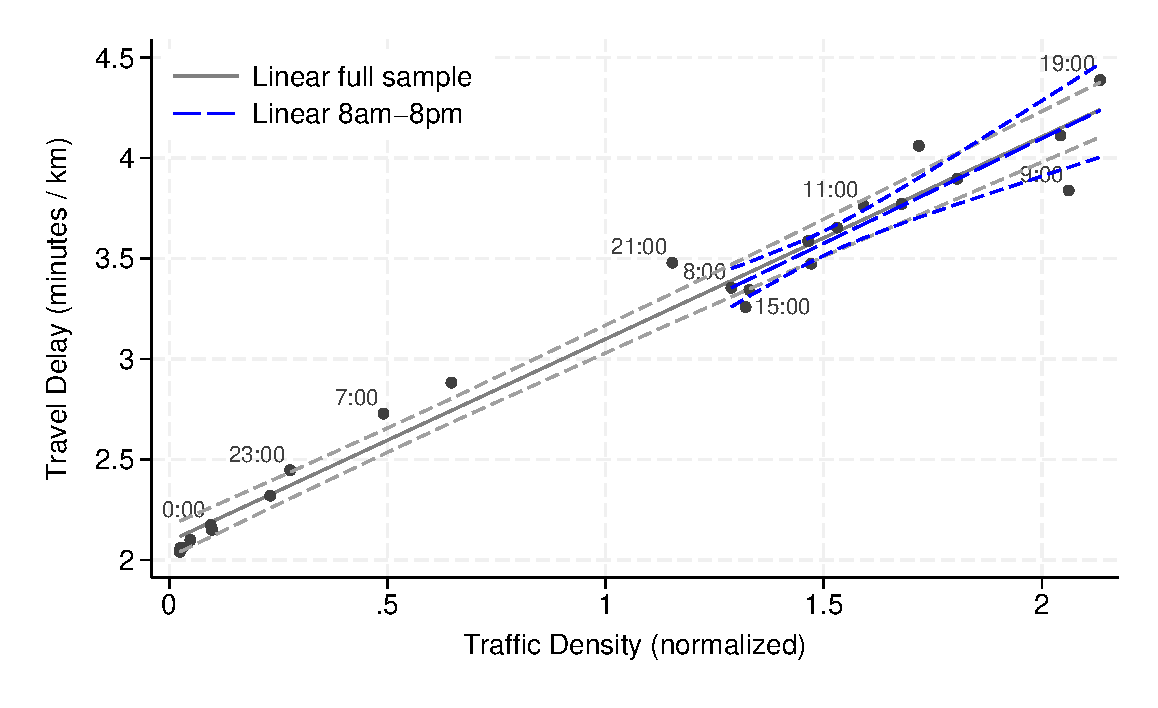
\includegraphics[scale=0.7]{"figures/figure4/figure_figure4_h.pdf"}
\par\end{centering}


\begin{singlespace}
{\small Notes: This graph shows that instantaneous travel delay is approximately linear in traffic density at the level of departure times. The traffic density measure uses GPS data for 140,574 trips from 1,774 app users on 185 weekdays. To compute traffic density, I count the total number of ongoing trips at any given minute of the day (on any day in the sample), on weekdays. I normalize by the number of trips and by $0.5\cdot 24$ because the average trip duration is close to 30 minutes. Travel delay is derived from Google Maps data collected over 30 routes in South Bangalore (in both directions), every 20 minutes daily for 185 weekdays. I compute the average delay over all weekdays and routes for each departure time. I plot the linear fit together with confidence intervals based on Newey-West inference with 3 hours lag, for the entire sample (gray, solid line) as well as for daytime hours only (blue, dashed line). Table \ref{tab:Road-Technology} reports corresponding regressions. Figures \ref{fig:road_tech_date} and \ref{fig:road_tech_artery} repeat this exercise separately for specific calendar dates, and for specific road arteries.  (\citealt{kreindler2023}, Figure A.5.) repeats this exercise at the level of calendar dates instead of departure times.  \par}
\end{singlespace}
\end{figure}\vspace{-0.25in}


\begin{figure}[H]

\caption{Policy Simulation: Unpriced Nash Equilibrium and Social Optimum \label{fig:Equilibrium-Optimal-Social}}

\medskip{}

\begin{centering}

\includegraphics[width=0.8\textwidth]{"figures/figure5/figure5.pdf"}

\par\end{centering}

\begin{singlespace}
{\small{}Notes: This graph shows the profile of average travel delay under the simulated Nash equilibrium (black, dashed line) and under the social optimum (red, solid line). The social optimum is a Nash equilibrium implemented with Pigouvian (equilibrium-consistent) charges given by marginal social cost, which depends on trip length and departure time (Figure \ref{fig:sims_additional}, panel A). To construct this figure, for each trip length $K$, I compute the trip travel time for each departure time, and divide it by $K$ to obtain travel delay. I then integrate over the trip length $K$ distribution. 	
	\par}
\end{singlespace}

\end{figure}\vspace{-0.25in}

\newpage{}




\section*{Tables}

\begin{table}[H]
\begin{centering}
\caption{Impact of Departure Time Charges on Daily Outcomes\label{tab:DT-daily}}
\par\end{centering}
\medskip
\begin{centering}
\begin{tabular}{lccc@{\hskip 0.25in}ccc}
\toprule
 & (1) & (2) & (3) & (4) & (5) & (6) \\
Outcome & \multicolumn{3}{c}{\textit{Total Hypothetical Rates Today}} & \multicolumn{3}{c}{\textit{Number of Trips Today}}  \\
Time of Day & AM \& PM & AM & PM   &   AM \& PM & AM & PM \\
Commuter FE & X & X & X & X & X & X \\
\addlinespace\addlinespace\multicolumn{7}{l}{\emph{Panel A. All Departure Time Sub-Treatments}} \\
\ExpandableInput{tables/table1/table_daily_panel_A}
\addlinespace\addlinespace\multicolumn{7}{l}{\emph{Panel B. Any Departure Time Charge vs. Control or Information}} \\
\ExpandableInput{tables/table1/table_daily_panel_B}
\bottomrule
\end{tabular}

\par\end{centering}
\medskip{}

\medskip{}

\begin{singlespace}
{\small{}Notes: This table reports difference-in-differences impacts of the departure time sub-treatments on daily total hypothetical rates and the total number of trips. In the first three columns, the outcome is the sum over trips that day of the trip hypothetical rate. The hypothetical rate for a given trip is between $0$ and $100$ and is computed based on the trip departure time, the respondent's rate profile, and a peak rate of 100 for all respondents. (See \citet{kreindler2023}, Figure A.2., for an example of rate profile.) In the last three columns, the outcome is the number of trips that day. The sample is all non-holiday weekdays with good quality GPS data, excluding days outside Bangalore. Only good quality trips are included (\citealp{kreindler2023}, section A.3.). In the post period, the sample is restricted to the departure time treatment period, either the first or the last three weeks. Columns (2), (4) and (3), (6) restrict to trips in the morning interval (7am--1pm) and the evening interval (4--10pm), respectively. ``Charges'' is a dummy for either low rate or high rate. All specifications include respondent and study cycle fixed effects, and $Post$ is an indicator for the experiment period. The mean of the outcome variable in the control group during the experiment is reported for each specification. Standard errors in parentheses are clustered at the respondent level. $^{*}p\leq0.10$, $^{**}p\leq0.05$, $^{***}p\leq0.01$ }
\end{singlespace}
\end{table}

\newpage{}










\begin{table}[H]

	\caption{Travel Demand Parameter Estimates\label{tab:gmm}}
	
	\medskip
	
	\begin{centering}
		\input{"tables/table2/table_main_gmm_4col"}
	\par\end{centering}
		
	\medskip{}

	\begin{singlespace}
	{\small Notes: This table reports two-step 	GMM estimates of discrete choice travel demand models. The estimating equation, moments, data and procedure are described in section \ref{sec:estimation}. Column 1 corresponds to the full model with departure time and dynamic route choice. Columns 2 and 3 use a departure time model with a single route (the short route, $r=0$) and calibrate VOTT to 50\% and 100\% of the average wage in the sample. The parameters $(\beta_E, \beta_L, \sigma^{DT})$ are estimated using the set of 49 departure time moments. Column 4 corresponds to a model of dynamic route choice without departure time choice, estimated using the set of 10 dynamic route choice moments. For each model, I use 120 random initial conditions to find the minimum of the objective function. 95\% confidence intervals from 120 bootstrap iterations are reported in parentheses.  \par}
	\end{singlespace}
\end{table}


\begin{table}[H]

	\caption{Road Technology Supply Estimation: Travel Delay Linear in Traffic Density \label{tab:Road-Technology}}
	
	\medskip
	
	\begin{centering}
		\input{tables/table3/rev2_table_table3_gm}
	\par\end{centering}

	\medskip{}
	
	\begin{singlespace}
	{\small
Notes: This table estimates the supply relationship between travel delay and traffic density in Bangalore. 
Columns 1 and 2 report 2SLS results where normalized density is instrumented with hour-of-day dummies, restricting to daytime 6am-10pm in column 2. I compute traffic density separately for each date, normalizing by the number of app users active in the same week. I report HAC standard errors with Newey-West kernel with a lag of 144 hours, and the effective F-stat and critical value with threshold 5\% (for worst-case relative bias) and significance level 5\%, from \citep{olea2013}. Columns 3 and 4 report results at the hour-of-day level (see notes for Figure \ref{fig:Road-Technology}). In column 4 I run the nonlinear regression $X_{h}=\lambda_{0}+\lambda_{1}(\widetilde D^S_{h})^{\nu} + \varepsilon_h$. Columns 3 and 4 report HAC standard errors with Newey-West kernel and three-hour lag. In column 5, I compute total traffic density on each date, and the regression reports HAC standard errors with Newey-West kernel and a 14-day lag. \citet{kreindler2023}, Table A.10., repeats the analysis using travel delay computed from GPS data. $^{*}p\leq0.10$, $^{**}p\leq0.05$, $^{***}p\leq0.01$
 \par}
	\end{singlespace}
\end{table}

\newpage{}

\begin{table}[H]

	\caption{Policy Simulations: Commuter Welfare Gains from Optimal Peak-Hour Pricing\label{tab:Social-Optimum}}
	
	\medskip
	
	\begin{centering}
		\begin{tabular}{lcccc}
\toprule
\addlinespace
& (1) & (2) & (3) & (4) \\ 
& Nash & \thead{Social \\ Optimum} &  Improvement & \thead{Improvement \\ (\% of Nash)} \\ 
\addlinespace\addlinespace 
\multicolumn{5}{l}{\emph{Panel A. Benchmark Model: Travel Time and Commuter Welfare}} \\ 
\addlinespace 
Travel Time (minutes) & 37.3 & 34.8 & 2.4 & 6.5\%  \\ 
 & (32.4,41.9)  & (30.3,38.7)  & (0.7,4.7)  & (1.9,12.0) \\ 
\addlinespace 
Travel Time above Free Flow & 14.1 & 11.7 & 2.4 & 17.1\%  \\ 
 & (11.0,17.7)  & (8.9,14.4)  & (0.7,4.7)  & (5.4,29.6) \\ 
\addlinespace 
Welfare (INR) & -392 & -383 & 8.9 & 2.2\%  \\ 
 & (-741,-190)  & (-715,-184)  & (1.7,31.3)  & (0.6,4.6) \\ 
\addlinespace 
Welfare above Free Flow (INR) & -157 & -148 & 8.9 & 5.7\%  \\ 
 & (-287,-90)  & (-260,-87)  & (1.7,31.3)  & (1.9,10.5) \\ 
\addlinespace 
\addlinespace 
\multicolumn{5}{l}{\emph{Panel B.  Preference Heterogeneity (Commuter Welfare, INR) }} \\ 
 \addlinespace 
Preferences $\propto$ wage & -527 & -508 & 18.3 & 3.4\%  \\ 
 & (-1373,523)  & (-1295,529)  & (3.1,79.1)  & (-1.0,7.2) \\ 
\addlinespace 
\addlinespace 
\multicolumn{5}{l}{\emph{Panel C. Varying Preferences (Commuter Welfare, INR) }} \\ 
 \addlinespace 
VOTT$\approx 100\%$ wage ($4\times$ smaller $\alpha$) & -112 & -110 & 1.2 & 1.1\%  \\ 
\addlinespace 
VOTT$\approx 1,600\%$ wage ($4\times$ larger $\alpha$) & -1434 & -1383 & 50.8 & 3.5\%  \\ 
\addlinespace 
High schedule cost ($4\times$ larger $\beta_E$) & -421 & -412 & 8.7 & 2.0\%  \\ 
\addlinespace 
Low schedule cost ($4\times$ smaller $\beta_E$) & -348 & -335 & 12.8 & 3.6\%  \\ 
\addlinespace 
\addlinespace 
\multicolumn{5}{l}{\emph{Panel D. Varying Road Technology (Commuter Welfare, INR) }} \\ 
 \addlinespace 
Concave Road Technology ($\nu=0.5$) & -369 & -369 & 0.3 & 0.1\%  \\ 
\addlinespace 
Convex Road Technology ($\nu=1.5$) & -434 & -387 & 46.3 & 10.7\%  \\ 
\addlinespace 
\addlinespace 
\multicolumn{5}{l}{\emph{Panel E.Equilibrium with Two Routes (Commuter Welfare, INR) }} \\ 
 \addlinespace 
One route 15\% steeper & -387 & -375 & 11.4 & 2.9\%  \\ 
\addlinespace 
One route 30\% steeper & -388 & -374 & 14.3 & 3.6\%  \\ 
\addlinespace 
\addlinespace 
   \bottomrule 
 \end{tabular} 


		\medskip{}
	\par\end{centering}
	
	\medskip{}
	
	\begin{singlespace}
		{\small{}Notes: This table compares the unpriced Nash equilibrium and the social optimum under different assumptions. Columns 3 and 4 report the improvement from the unpriced Nash to the social optimum, in levels and as a percentage of the baseline (Nash) value. Panel A describes the benchmark model with preferences as estimated from the experiment and the calibrated road technology. Travel times are calculated taking individual route length into account, and welfare is average expected utility, assuming charges are transferred lump-sum back to commuters, and no implementation costs. In rows 2 and 4 travel time and welfare are computed relative to ``free-flow'' benchmark, where travel delay is 2.09 min/km and does not increase with traffic density. Agent preferences in Panel B correspond to those estimated in column 5 in Table \ref{tab:gmm-other}. In Panel C, I vary the VOTT or early schedule cost parameters. In Panel D, I vary the exponent on traffic density in the road technology relationship (Figure \ref{fig:sims_additional}, panel C). In panel E, I simulate a model with two routes that have different road technologies. Route $r=0$ has the benchmark road technology, while $r=1$ has 15\% or 30\% steeper slope and $7.5\%$ or $15\%$ lower intercept. In panels A and B, 95\% confidence intervals are bootstrapped based on bootstrapped parameter vector estimates, and random draws from the road technology variance covariance matrix (Table \ref{tab:Road-Technology}, column 1).\par}
	\end{singlespace}
\end{table}

\newpage{}


\begin{table}[H]

\caption{Policy Simulations: Equilibrium with Extensive Margin Decision \label{tab:Social-Optimum-Extensive}}

\medskip

\begin{centering}
	\begin{tabular}{cccccc} 
\toprule 
\addlinespace 
\thead{Trip value \\ $ \omega $} & \thead{Logit trip \\ parameter \\ $ \eta $} & \thead{ \% Traffic Reduction \\ from flat 100 INR fee }  & \thead{Implied elasticity \\ at flat 100 INR fee} & \thead{ Nash \\ Welfare (INR)} & \thead{Improvement \\ at Social Optimum \\ (\% of Nash)} \\  
\addlinespace\addlinespace 
600 INR & 20 & -0.31 & 1.26 & -393.7 & 4.4\% \\ 
\addlinespace
800 INR & 20 & -0.08 & 0.25 & -393.9 & 2.2\% \\ 
\addlinespace
1000 INR & 20 & -0.01 & 0.02 & -393.9 & 2.2\% \\ 
\addlinespace
600 INR & 100 & -0.25 & 1.0 & -359.3 & 4.3\% \\ 
\addlinespace
800 INR & 100 & -0.12 & 0.4 & -387.2 & 3.4\% \\ 
\addlinespace
1000 INR & 100 & -0.04 & 0.11 & -392.9 & 2.5\% \\ 
\addlinespace
   \bottomrule 
 \end{tabular}  


\medskip{}
\par\end{centering}
\begin{centering}
\medskip{}
\par\end{centering}
\begin{singlespace}
{\small{}Notes: This table reports commuter welfare gains from optimal congestion pricing and extensive margin elasticities for the model with an extensive margin trip decision (Supplementary Material \ref{app-sims}). The implied elasticity is computed with respect to total travel costs (equal to negative commuter expected welfare) at the Nash equilibrium. The average trip probability is $\geq 97\%$ at the Nash equilibrium for all parameter combinations except for $\omega=600$ INR and $\eta=100$, when it is $89\%$. In these simulations, average congestion charges at the social optimum vary between 95 INR and 190 INR.

\par}
\end{singlespace}
\end{table}

\newpage{}

\begin{appendices}

\renewcommand\thesection{SM}

\section{Supplement to ``Peak-Hour Road Congestion Pricing: Experimental Evidence and Equilibrium Implications''}
\DoToC

\renewcommand{\theHfigure}{SM\arabic{figure}} 
\renewcommand{\thefigure}{SM\arabic{figure}}
\setcounter{figure}{0} 

\subsection{Departure Time Model Identification
\label{sec:model-identification}
}

In this section, I formally prove how identification of schedule costs and schedule heterogeneity in a departure time model depends on observing commuter reactions to congestion pricing. For analytical tractability, I proceed in a simplified model that maintains the key features of the full model: schedule preferences and a peak-hour (inverse U shaped) travel time profile. These results continue to hold when the travel time profile is endogenously determined in equilibrium. I use simulations to check a conjecture that the deadweight loss of peak-hour congetion in this model is decreasing in the schedule costs.

For intuition for the identification results, consider a commuter that we observe to leave at very different times on different days (as I document in Table \ref{tab:Descriptive-Statistics-about}). There are two ways this could arise. In the first scenario, the commuter has a unique ideal arrival time and high schedule flexibility. In this case, small idiosyncratic shocks have a large effect on departure times. In the second scenario, each day, the commuter draws an ideal arrival time from a dispersed distribution, but does not have much flexibility around that time.

These two cases are observationally equivalent for departure times, but they have different implications for how substitutable two departure times are to each other, on any given day. The key intuition for how congestion pricing leads to identification is that we can measure cross-price elasticities: how the probability of choosing departure time $h$ depends on infinitesimal pricing of departure time $h'$.

\subsubsection{Simplified Departure Time Model}
I assume that commuters have preferences directly over (continuous) departure times $h\in\mathbb R$. Unlike the main model where commuters have ideal \textit{arrival} times, this assumption eliminates expectations over travel time uncertainty and greatly simplify the algebra. 

Travel time is a (possibly degenerate) quadratic function of departure time. This captures the key shape of how travel time varies across the peak hour.\footnote{The quadratic shape implies unrealistic negative travel time for very early or very late departure time. I later assume that schedule costs rise faster so that, on net, these departure times are unattractive.}  In most of the results below, schedule costs are quadratic and the ideal departure time is normally distributed. These assumptions rule out asymmetric (early/late) schedule costs yet deliver analytical tractability.

Given the focus on identification, I drop individual $i$ and time $t$ subscripts and assume that infinite data for a single individual is available. The utility for departure time $h$ is

$$\underbrace{-\alpha T(h)-v(h-h^D)}_{u(h|h^D)}+\epsilon^D(h).$$

Here $v(\cdot)$ is the schedule penalty as a function of the deviation between departure time and the ideal departure time $h^D$. $\epsilon^D(h)$ are idiosyncratic shocks with scale $\beta^{-1}$ that give rise to continuous logit choice probabilities. The ideal departure time $h^D$ is distributed according to a cumulative distribution function $F$. 

I assume that the value of travel time $\alpha$ is known and normalize it to $\alpha=100$ INR/hour. Note, if travel time is not constant, this rules out a trivial source of non-identification due to scale.

The conditional probability density of choosing departure time $h$ is given by the continuous logit density, and the unconditional density is given by integrating over $F$,

\begin{equation*}
	\pi(h|h^D)=\frac{\exp(\beta u(h|h^D))}{\int_{h'} \exp(\beta u(h'|h^D))dh'},
	\text{ and}\quad
	\pi(h)=\int\pi(h|h^D) dF(h^D).
\end{equation*}


\subsubsection{Two Non-Identification Results with Observational Data}
Before outlining the main results, I prove a general non-identification result in a simple setting where travel time is a constant (later, I will assume quadratic) and the ideal departure time distribution is unrestricted. 

In this case, we can write the observed departure time as the sum of two independent random variables, corresponding to the ideal departure time, and the optimal departure time conditional on the ideal departure time. This exact decomposition helps clarify the source of non-identification.

\begin{prop}
	Assume that travel time $T$ is a constant (does not depend on departure time $h$). Normalize $\beta=1$. Consider any family $V$ of schedule delay functions $v\in V$, with at least two elements $v_1,v_2\in V$ that differ on a non-zero measure set. Then, the schedule delay cost function $v(\cdot)$ is not identified given data on $\pi(h)$. 
\end{prop}

\begin{proof}
If $T$ does not depend on $h$, then $u(h|h^D)$ is only a function of the difference $h-h^D$. Hence, the optimal departure time random variable $h^*$ can be written as the sum of two independent random variables, $h^*=h^D+\underbrace{h^*-h^D}_{h^E}$, where the pdf of $h^E$ is

$$G(h^E)=\frac{\exp(-v(h^E))}{\int_{h} \exp(-v(h))dh}.$$

(Note: if $v$ is quadratic then $h^E$ is normally distributed.)

Consider two different schedule delay functions $v_1(\cdot)$ and $v_2(\cdot)$ and let $h^E_1$ and $h^E_2$ denote two independent random variables that have the corresponding pdfs $G_1$ and $G_2$. 

Setting the ideal departure time distributions $h^D_1\sim G_2$ and $h_2^D\sim G_1$ (note that indices are switched) implies that the observed optimal departure time random variables $h^D_1+h^E_1$ and $h_2^D+h^E_2$ have the same distribution. Hence, the schedule cost function $v(\cdot)$ is not identified. 
\end{proof}

The identification failure does not depend on constant travel time. I next prove the main non-identification result, in a model that is more strongly parametrized and where travel time is hump-shaped, which captures the peak-hour travel time profile. I make three functional form assumptions.

\textbf{Assumption 1.} $T(h)$ is quadratic, $T(h)=\tau_0-\tau_1 h^2$ with $\tau_1 >0$. Without loss of generality and for convenience I will set $\tau_0=0$.

\textbf{Assumption 2.} Schedule costs are quadratic, $v(h-h^D)=s(h-h^D)^2$ with $s>\tau_1 $.

($s>\tau_1 $ means that schedule costs dominate, and it implies that the commuter chooses departure times with negative travel time--very early or very late departure time--with very low probability.)

\textbf{Assumption 3.} The ideal departure time is normally distributed, $h^D\sim N(0,\sigma)$.

\begin{prop}
	\label{prop:notid}
	Fix the shape of the travel time profile $\tau_1$ and maintain the VOTT normalization $\alpha=100$ INR/hour. Under assumptions 1--3, the demand model parameters $(\beta,s,\sigma)$ are not identified with data on observed departure times.
\end{prop}

This is not a trivial non-identification result due to scale, because VOTT $\alpha$ is normalized, and travel time is not constant.

The proof will show that it is possible to explain the same observed distribution of departure times by increasing schedule costs and increasing the spread of the ideal departure time distribution.

\begin{proof}[Proof of Propostion \ref{prop:notid}]
	I show that $\pi(h)$ is a normal distribution centered at zero. Its mean and variance depend on three variables ($\beta,s,\sigma$). Hence, the model is under-identified with two degrees of freedom.
	
	The utility functions is (recall that the value of time spent driving $\alpha$ is normalized)
	
	$$u(h|h^D)=\alpha\tau_1h^2-s(h-h^D)^2+\epsilon^D(h).$$
	
	Choice probabilities are given by
	\begin{align*}
		\pi(h) &= \int \pi(h|h^D)dF(h^D)\\
			    &= \int  \frac{e^{-\beta  \left(-\alpha\tau_1 h^2+s (h-h^D)^2\right)}}{\int_{-\infty }^{\infty } e^{-\beta  \left(-\alpha\tau_1 (h')^2+s (h'-h^D)^2\right)} \, dh'}
		\cdot
		\frac{1}{\sqrt{2 \pi } \sigma } e^{-\frac{1}{2} \left(\frac{h^D}{\sigma }\right)^2} dh^D \\
		&=  
		\frac{1}{\sqrt{2 \pi } \sqrt{\frac{s^2 \sigma ^2}{(s-\alpha\tau_1)^2}+\frac{1}{2 \beta  (s-\alpha\tau_1)}}}
		\exp \left(-\frac12\frac{h^2}{ \frac{s^2 \sigma ^2}{(s-\alpha\tau_1)^2}+\frac{1}{2 \beta  (s-\alpha\tau_1)}}\right).
	\end{align*}
	
	This is a normal distribution with mean zero and variance $\frac{s^2 \sigma ^2}{(s-\alpha\tau_1)^2}+\frac{1}{2 \beta (s-\alpha\tau_1)}$. 
\end{proof}


\subsubsection{Identification with Congestion Pricing Variation}
I now study identification when we also observe choice probability distributions $\pi(\cdot|p(\cdot))$ in response to any possible pricing function $p(h)$.

Observing responses to pricing helps identify the cross-price elasticities for different departure times. This helps resolve the ambiguity discussed in the previous section, because different combinations of departure time distributions and conditional choice probabilities have different implications for cross-price elasticities.

The key object of interest is the impact of an ``impulse'' price function on choice probabilities. Slightly abusing notation (skipping a formal limit argument), we study ``Kronecker delta'' impulse pricing functions at $h$ given by $p(x;h,\lambda)=\lambda 1(x=h)$ and study the effect of increasing $\lambda$ around $\lambda=0$ for given $h\neq h'$:

$$\left.\frac{d\pi(h'|p(\cdot;h,\lambda))}{d \lambda}\right|_{\lambda=0}=
\frac{d}{d \lambda}
\int
\frac{\exp(\beta u(h'|h^D))}{\int_{h''} \exp(\beta u(h''|h^D) - \beta p(h'';h,\lambda))}
dF(h^D).$$

For $h\neq h'$ and evaluating at $\lambda=0$ this simplifies to

$$\beta\int 
\pi(h'|h^D)\pi(h|h^D)
dF(h^D),$$

where $\pi(\cdot|h^D)$ denotes the conditional probability in the absence of pricing ($\lambda=0$).

This expression shows that, for fixed $h-h'$, when conditional probabilities are concentrated (e.g. when $\beta$ is high and/or the schedule cost function is steep around the ideal departure time), the cross-elasticities are close to zero. Intuitively, this suggests that knowing cross-elasticities for all $h$ and $h'$ solves the identification problem.

I now formally prove identification in the particular case considered in Result 2.

\begin{prop}
	Fix the shape of the travel time profile $\tau_1$. Under assumptions 1--3, the model parameters $(\beta,s,\sigma)$ are identified with data on observed departure times and cross-elasticities for $h\neq h'$.
\end{prop}

\begin{proof}
	Substituting the utility function and normal distribution for $h^D$ in the expression for cross-elasticity, and computing integrals using Mathematica, yields
	
\begin{align*}
		\beta\int\pi(h'|h^D)\pi(h|h^D)dF(h^D) &= \beta^2(s-\alpha\tau_1)^{\frac12}
		\left(s-\alpha\tau_1+4 \beta  s^2 \sigma ^2\right)^{-\frac 12} \\
		& \exp \left(
		\frac{(s-\alpha\tau_1) 2 \beta^2  s^2 \sigma ^2 }{\left(s-\alpha\tau_1+4 \beta  s^2 \sigma ^2\right)}(h'+h)^2
		-(s-\alpha\tau_1) \beta  \left((h')^2 + h^2\right)\right).
\end{align*}
	
	Taking log and grouping terms in a polynomial of $h$ and $h'$ gives
\begin{align*}
		\ln\left(\int\pi(h'|h^D)\pi(h|h^D)dF(h^D)\right) = 
		&-\beta  (s-\alpha\tau_1) ((h')^2+h^2)+ \\
		&\frac{ 2 \beta ^2 s^2 \sigma ^2 (s-\alpha\tau_1)}{s-\alpha\tau_1+4 \beta  s^2 \sigma ^2}(h'+h)^2+ \\
%		&\ln(\beta ) + \frac{1}{2} \ln(s-\alpha\tau_1) -\frac{1}{2} \ln\left(s-\alpha\tau_1+4 \beta  s^2 \sigma ^2\right).
		&\frac{1}{2}\ln\left(\frac{\beta^2(s-\alpha\tau_1) }{s-\alpha\tau_1+4 \beta  s^2 \sigma ^2}\right).
\end{align*}
	
By varying $h$ and $h'$, we have three identified coefficients and three unknowns ($\beta$, $s$, and $\sigma$). It is straightforward to check that this system of equations has a unique solution.
\end{proof}

\subsubsection{Equilibrium with Endogenous Congestion}
I now show that the quadratic travel time profile assumed so far is consistent with equilibrium.

Assume that the travel time $T(h)$ is given by
\begin{equation}
	\label{eq:normal_model_road_tech}
	T(h)=\lambda_0 + \lambda_1\log(V(h)),
\end{equation}
where $V(h)$ a measure of volume of travel around $h$. To construct $V$, assume that any trip at $h$ affects the travel times of all other departure times (trips leaving both before and after $h$), with a weight given by a normal distribution pdf with standard deviation $\sigma_V$. That is, $V$ is given by
$$
V(h)=\int_{-\infty}^\infty \pi(h')\phi(h';h,\sigma_V)dh',
$$
where $\phi(x;\mu,\sigma)$ is the normal pdf with mean $\mu$ and standard deviation $\sigma$, evaluated at $x$.

Given that $\pi$ is a normal pdf, so will $V$, and hence travel time given by \eqref{eq:normal_model_road_tech} will be quadratic in $h$. 
\begin{prop}
	This model has a unique equilibrium, where travel time is quadratic and choice probabilities follow a normal pdf. The following equilibrium equation holds:
\begin{equation*}
	\frac{s^2\sigma^2}{(s-\alpha\tau_1)^2} + \frac 1{2\beta(s-\alpha\tau_1)}+\sigma_E^2=\frac{\lambda}{2\alpha\tau_1}.
\end{equation*}
\end{prop}

\subsubsection{The Deadweight Loss of Congestion is Decreasing in Schedule Costs\label{sec:app-model-dw}}
Consider an equilibrium as described above. Based on Proposition \ref{prop:notid}, the observed choice probabilities and travel time profile are consistent with various combinations of schedule cost $s$ and dispersion of ideal departure times $\sigma$. 
\begin{conj}
	Holding fixed the equilibrium choice probabilities $\pi(h)$ and the profile of travel time $T(h)$, the deadweight loss of congestion (in absolute terms) is decreasing in schedule costs $s$.
\end{conj}

The deadweight loss does not appear to have a closed form solution. I use numerical simulations for 1,000 randomly chosen parameter vectors. I maintain the normalization $\alpha=100$ INR/hour, and draw the following parameters uniformly and independently: $s\in [25,125]$ INR/hour$^2$, $\sigma\in[0.05, 0.55]$ hours, $\beta\in[0.25,0.75]$, $\sigma_V\in[0.5, 1,5]$ hours, and $\lambda_1\in[1.5, 2.5]$. In each simulation, I choose 10 alternate possible values of $s'$ and solve for the implied $\sigma'$ that leads to the same equilibrium as with the initial $s,\sigma$, and compute deadweight loss. In all 1,000 simulations, deadweight loss is decreasing in $s'$.

\begin{figure}[H]
	\centering
	\includegraphics[width=0.5\textwidth]{"figures/smfigure1/example_dw_sch_cost.pdf"}
	\caption{Example deadweight loss versus schedule cost (holding observed equilibrium fixed)}
\end{figure}


\subsection{Route Choice Model Identification\label{app:vott-id}}
To provide intuition for how VOTT and the route switching cost are separately identified using data from the route choice experiment, I analyze a version of the dynamic route choice model without departure time from section \ref{subsec:dynamic-route-choice}. I further assume no time discounting ($\delta=0$).

Consider three time periods. At $t=0$ the model is in steady state. At $t=1$ the short route ($r=0$) is unexpectedly charged $p$. At $t=2$ the route is no longer charged. Denote $\pi_t(r_{t-1}\to r)$ the probability to use route $r$ at time $t$ if the $t-1$ route was $r_{t-1}$ when there is no pricing, and $\pi_t(r_{t-1}\to r|p)$ with pricing $p$. Because there is no discounting, we have the following expressions for relative transition probabilities:
\begin{align*}
	\frac{\pi_0(0\to0)}{1-\pi_0(0\to0)} = \frac{\exp(0)}{\exp(\frac{-\gamma-\alpha\Delta T}{\mu})} &\quad\quad \frac{\pi_0(1\to0)}{1-\pi_0(1\to0)} = \frac{\exp(\frac{-\gamma}{\mu})}{\exp(\frac{-\alpha\Delta T}{\mu})} \\
	\frac{\pi_1(0\to0|p)}{1-\pi_1(0\to0|p)} = \frac{\exp(\frac{-p}{\mu})}{\exp(\frac{-\gamma-\alpha\Delta T}{\mu})} &\quad\quad \frac{\pi_1(1\to0|p)}{1-\pi_1(1\to0|p)} = \frac{\exp(\frac{-p-\gamma}{\mu})}{\exp(\frac{-\alpha\Delta T}{\mu})}.
\end{align*}
It is easy to solve for the parameters $\alpha,\gamma,\mu$ if these transition probabilities are known. Next, I show that these parameters are also unique determined by the detour route usage rates $S_t$ in periods $t=0,1,2$. These numbers satisfy the following equations (note that $t=0$ and $t=2$ have the same transition probabilities)
\begin{align*}
	S_0\pi_0(0\to 1) &= (1-S_0)\pi_0(1 \to 0) \\
	S_1 &= S_0\pi_1(0 \to 0|p) + (1-S_0)\pi_1(1\to 0|p) \\
	S_2 &= S_1\pi_0(0 \to 0)   + (1-S_1)\pi_0(1\to 0).
\end{align*} 
It is tedious but straightforward to show that these three equations uniquely determine $\alpha,\gamma,\mu$.




\subsection{Route Charge Treatment Regression Analysis\label{app:route-reg}}
For the regression analysis of the route experiment, I focus on the early treatment group and the period before the experiment and the first two weeks during the experiment. I use the following specification:\vspace*{-0.5cm}

\begin{equation}
	\label{eq:area-spec}
	y_{it} =
	\gamma^{A}\cdot T_{i}^{Early}W_t^1 +
	\gamma^{A,P}\cdot T_{i}^{Early}W_t^2 +
	\mu_{t}+\alpha_{i}+\varepsilon_{it}.
\end{equation}

The coefficients of interest are $\gamma^{A}$ and $\gamma^{A,P}$, which measure the impact of route congestion charges in the early charges group, and the persistence effect one week later, relative to similar commuters who anticipate that they will be treated in the fourth week of the experiment.

Panel A of Table \ref{tab:A-daily} shows the impact of route charges on detour usage at the trip level. The sample is all trips between home and work. The results show a large increase of 27 percentage points during the first week in the experiment among the early treatment group, who faced charges that week. By comparison, only 11\% of participants in the late group chose the detour that week. The second column shows that more than a third of this effect size persists one week later. Charges do not have a significant effect on the number of trips per day (columns 3 and 4). This means that there is no evidence that commuters reduce the number of trips to avoid route congestion charges, and the previous effects are driven by route switching.

I next analyze how baseline experience with detour routes affects the impact of charges. In Panel B, I restrict to commuters who use a detour route between home and work (or between work and home) at least once before the experiment. In general, the results from Panel A are amplified in this sample. Baseline usage is higher, as are the impact of charges (41 percentage points) and the persistence effect. 





\subsection{Travel Demand Estimation}
\label{sec:model-struct}

\subsubsection{Choice Probabilities}
\label{subsec:model-choice-probs}

In the benchmark model with dynamic route choice and departure time choice, the departure time choice probabilities conditional on the chosen route (with $p_{it}(h,r)=0$) is given by
\begin{equation*}
	\label{eq:choice-probs-conditional}
	\pi_{i}(h|r, h_{it}^A) = \frac{\exp((\sigma^{DT})^{-1}\mathbb{E} v(h,\mathcal T_{i}(h,r), h_{it}^A))}{\sum_{h'} \exp((\sigma^{DT})^{-1}\mathbb{E} v(h',\mathcal T_{i}(h',r), h_{it}^A))}.
\end{equation*}
These expressions show that the full model collapses to the single-route departure time choice model given by \eqref{eq:utility-1-route} when we condition on route and ideal arrival time. Similar expressions apply when we include pricing $p_{it}(h,r)$.

In the full model, the expected utility of choosing route $r$ is
\begin{equation*}
	\mathbb{E}u_{it}(r | h_{it}^A, r_{it-1}) = \sigma^{DT}\log
	\left(
	\sum_{h} \exp\left((\sigma^{DT})^{-1}\mathbb{E} v(h,\mathcal T_{i}(h,r), h_{it}^A)\right)
	\right)
	- \gamma \mathbf{1}(r\neq r_{it-1}) + \delta V_{it+1}(r).
\end{equation*}
This includes the ``logsum'' or `inclusive value'' term over departure times. In the upper nest, this leads to route choice probabilities (conditional on $h_{it}^A$)
\begin{equation*}
	\pi_{it}(r | h_{it}^A, r_{it-1}) = 
	\frac{
		\exp((\sigma^R)^{-1} \mathbb{E}u_{it}(r | h_{it}^A, r_{it-1}))
	}{
		\exp((\sigma^R)^{-1} \mathbb{E}u_{it}(0 | h_{it}^A, r_{it-1})) + 
		\exp((\sigma^R)^{-1} \mathbb{E}u_{it}(1 | h_{it}^A, r_{it-1}))
	}.
\end{equation*}
Unconditional probabilities follow by integrating over the ideal arrival time distribution $f_i^A$.



\subsubsection{GMM Moments That Exploit Experimental Variation}
\label{appsec:model-struct-moments}

The two-step optimal GMM estimation finds the parameter vector $\theta=(\alpha, \beta_E, \beta_L, \gamma, \sigma^{DT}, \sigma^R, \eta_\text{early})$ that solves $\min_\theta \hat g(\theta)'\hat W\hat g(\theta)$ where the moment function $g(\theta)$ is described below, and $\hat W$ is the estimated optimal weighting matrix from the second step. (For the first step I use $\hat W=I$.)

\textbf{Departure Time Moments.} The first 49 moments match the difference in difference in departure time market shares, between the departure time treatment and control groups, during the experiment relative to before. Let $k$ index the 5-minute-step departure time grid between $-120$ and $+120$ minutes relative to the rate profile peak. Denote $P_{ik}^{DT}(\theta, p_{it})$ the probability that the $k$th departure time is optimal when departure time and route pricing is $p_{it}$. In the data, define $\widetilde{P}_{ik}^{DT}\left(pre\right)$ and $\widetilde{P}_{ik}^{DT}\left(post\right)$ the fractions of trips starting in a 5-minute bin around the $k$th departure time for $i$ in pre- and post- periods, respectively. The $k$-th moment is:\vspace*{-0.2cm} 
\begin{equation*}
	g_i^{k}(\theta, p_{it}) = (-1)^{1-T_{i}^{DT}}\left[
			\left(\widetilde{P}_{ik}^{DT}(post)-\widetilde{P}_{ik}^{DT}(pre)\right) -
			 \left(P_{ik}^{DT}(\theta, p_{it}) - P_{ik}^{DT}(\theta, 0) \right)
 			 \right],
\end{equation*}

where $T_{i}^{DT}$ is an indicator for departure time charges.

\textbf{Route Moments.} Ten moments match route choice market shares during five periods (before the experiment, and four weeks during the experiment) indexed by $t=1,\dots,5$ and in two treatment groups (early and late charges).

Denote $P_{it}^{A}(\theta,p_{it})$ the probability to take the detour route (not intersect the congestion area) in time period $t$ when pricing is $p_{it}$. In the data, define $\widetilde{P}_{it}^{A}$ the fraction of days when commuter home-work trips do not intersect the congestion area for individual $i$, which depends on $i$'s treatment group. For $t=1,\dots,5$, the route moments are:\vspace*{-0.2cm}
\begin{align*}
	g_{i}^{49+t}(\theta, p_{it}) & = T_i^{Early}\cdot\left[ \widetilde{P}_{it}^{A} - P_{it}^{A}(\theta, p_{it}) \right]\\
	g_{i}^{54+t}(\theta, p_{it}) & = (1-T_i^{Early})\cdot\left[ \widetilde{P}_{it}^{A} - P_{it}^{A}(\theta, p_{it}) \right].
\end{align*}




\subsection{Parameter Sensitivity Measure\label{app:sensitivity}}
Table \ref{fig:gmm_diagnostics} reports the estimated sensitivity measure $\Lambda$ from \citet{andrews2017}, scaled by the  standard deviation of each moment. Each entry $\Lambda_{pj}$ measures the change in estimated parameter $\theta_{p}$ due to a one standard deviation change in moment $m_{j}$. The measure is $\hat{\Lambda}=\left(\hat{S}^{'}\hat{W}\hat{S}\right)^{-1}\hat{S}^{'}\hat{W}\mbox{diag}\left(\hat{\sigma}\right)$ where $\hat{S}$ is the Jacobian evaluated at the estimated parameters, $\hat{W}$ is the optimal weighting matrix, and $\hat{\sigma}$ is the vector of bootstrap standard deviation of moment $j$.


\subsection{Road Technology Invariance Result}
\label{app:road-tech}

Conditional on the relationship \eqref{eq:road-tech} estimated on a representative sample, the impact of an additional trip on total driving time in Bangalore is invariant to the aggregate volume of traffic in Banglore, and it is invariant to the sample size used to estimate the road technology relationship.

The key intuition is that equation \eqref{eq:road-tech} depends on normalized density, so it is invariant to the true aggregate volume of traffic. Then, imagine that the aggregate volume is twice as large as initially believed. Then the impact of a single trip on travel delay will be twice as small. However, it will affect twice as many other commuters, so the impact on total time is not affected.

Using the notation from section \ref{sec:model-road-tech-eqm}, let $Q=(q(h,K))_{h,k}$ denote the pattern of departures, where $q(h,K)$ is the mass of trips of length $K$ starting at $h$, based on a sample of $N$ trips. Let $x=(x(h))_h$ denote the instantaneous travel delay profile, and $d=(d(h))_h$ the density profile. Similar to equation \eqref{eq:road-tech}, assume that instantaneous delay satisfies $x(h) = \lambda_0+\lambda_1d(h)/N$ where $N$ is the number of trips in the sample. 


\begin{prop}
	The marginal effect of an additional trip on total travel time does not depend on the sample size used to construct $Q$.
\end{prop}
\begin{proof}
	Let $d(h',Q)$ denote density at time $h'$ as a function of the pattern of departures, and $d(Q)=(d(h',Q))_{h'}$. 
	
	Travel times are uniquely determined by the instantaneous travel delay profile, which depends on normalized density. Hence, we can write average travel times as a function $\overline T\left(\frac{d(Q)}{N}\right)$. Note that total travel time in the city is $N \overline T$.
	
	For every $h'$, $d(h',Q)$ is homogeneous of degree 1 in $Q$. Consequently, the partial derivative $d_{h,K}(h', Q)$ with respect to the mass of trips with length $K$ starting at $h$ is degree 0 in $Q$, i.e. it does not depend on the sample size used to compute $Q$.
	
	Consider adding a trip of length $K$ that starts at $h$ and denote the pattern of departures by $Q+\mathbf{1}(h,K)$. The change in \textit{total} travel time is
	
	$$
	N\left(\overline T\left(\frac{d(Q+\mathbf{1}(h,K))}{N}\right)    - \overline T\left(\frac{d(Q)}{N}\right)\right) 
	\approx 
	N\frac{\partial\overline T}{\partial\mathbf{1}(h,K)}
	=
	N\sum_{h'} \frac{\partial \overline T}{\partial h'} \frac{d_{h,K}(h',Q)}{N}
	$$
	
	The last term does not depend on $N$ because neither $\frac{\partial \overline T}{\partial h'}$ nor $d_{h,K}(h', Q)$ depend on $N$.
\end{proof}


\subsection{Policy Simulations}
\label{app-sims}

For policy simulations I use a 5-minute departure time grid from 5am to 2pm. Each simulation has 3040 agents, with each real study participant replicated with 10 independent random draws of ideal arrival times from the distribution recovered with non-negative least squares (section \ref{estimation-solving-model}). The vector of ideal arrival times is re-sampled during bootstrapping. Thus, the confidence intervals include uncertainty due to numerical simulation. Benchmark results are robust to using $10\times$ more agents.


For the two-route equilibrium model, I assume double the volume of trips, so that on average the volume of trips per route remains the same.

I use a nested logit model for the equilibrium model with an extensive margin decision. The outer nest has two options, taking the trip ($z=1$) and not taking the trip ($z=0$). Trips are valuable: a commuter not making a trip incurs a cost proportional to trip length $\omega_i=\omega\cdot \mathrm{K}_i/{\overline{\mathrm{K}}}$. Expected utility is given by:

\begin{equation*}
	\label{eq:expected-utility-extensive}
	\mathbb{E} u_i(x,h,h_i^A)=
	\begin{cases}
		\mathbb{E}v(h,\mathcal{T}_i(h), h_{it}^A) -p_{it}(h)+\varepsilon_{it}(1,h)  & z=1 \\
		-\omega_i + \varepsilon_i(0,h) & z=0
	\end{cases}
\end{equation*}
where $\varepsilon_i(z,h)$ follow a type-1 extreme value distribution with correlation within each value of $z$, with logit scale parameter $\eta$ for the trip (upper) nest. The congestion pricing experiment was not designed to estimate the extensive margin trip elasticity.




\subsection{Supplementary Material: Figures}





\begin{figure}[H]
	\caption{Impact of Departure Time Charges on Departure Times (Commuting Trips)\label{fig:DT-graphs-HW}}
	
	\medskip
	
	\makebox[\textwidth][c]{
		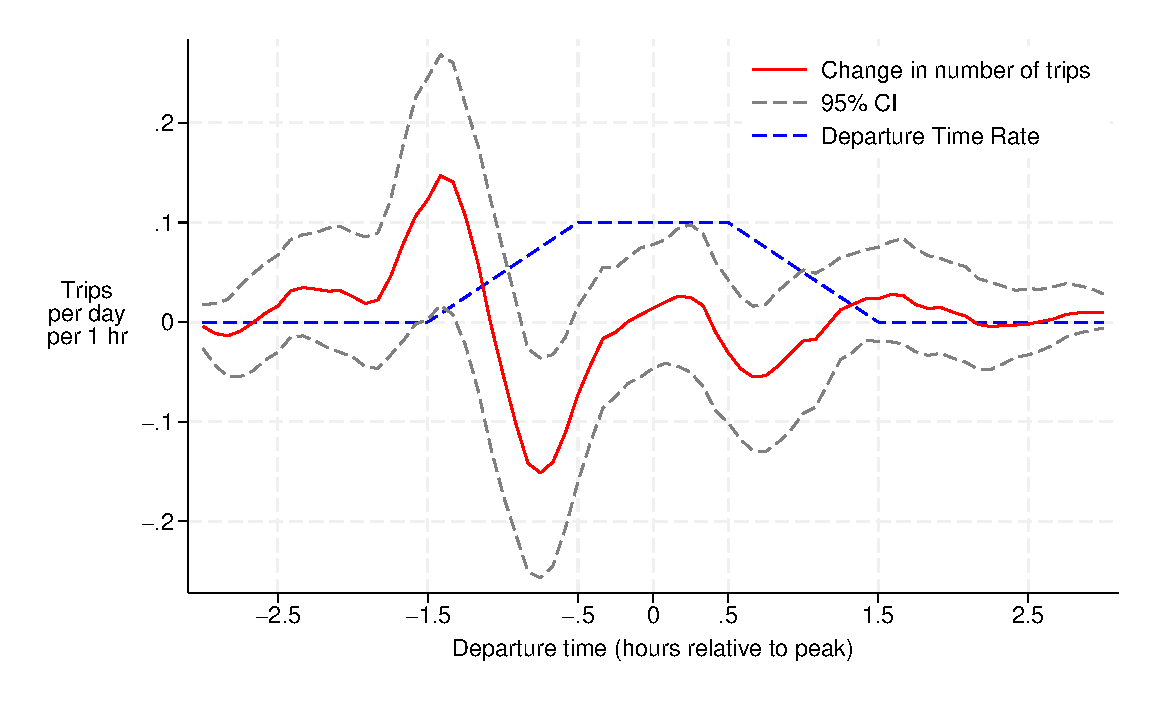
\includegraphics[width=0.55\textwidth]{"figures/figure2/figure_bw15_boot1000_hw_am.pdf"}
		
		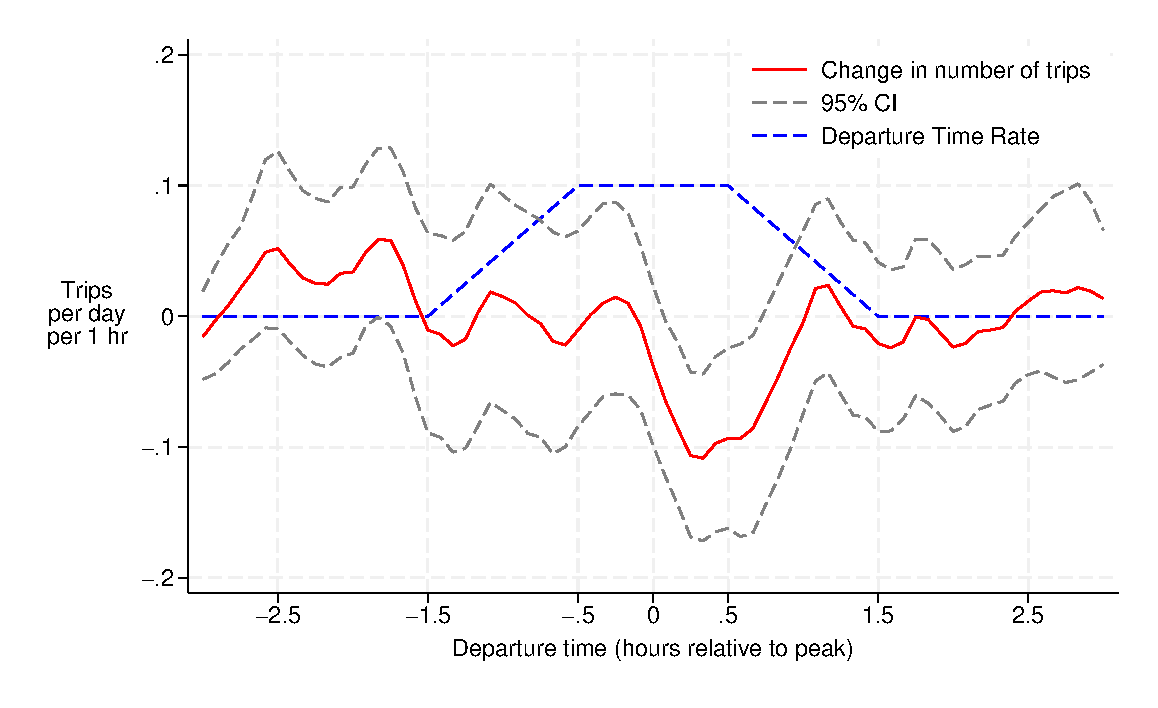
\includegraphics[width=0.55\textwidth]{"figures/figure2/figure_bw15_boot1000_hw_pm.pdf"}
		
	}

	\begin{centering}
		\quad\quad\quad\quad
		Panel (A) Morning Peak
		\quad\quad\quad\quad\quad
		Panel (B) Evening Peak
		\medskip
	\par\end{centering}
	
	
	\begin{singlespace}
		{\small Notes: Version of Figure \ref{fig:DT-graphs} restricting to regular commuters and trips between home and work (both ways).}
	\end{singlespace}
\end{figure}

\newpage{}


\begin{figure}[H]
	
	\caption{Travel Demand Model Fit }
	
	\bigskip
	
	\label{fig:gmm_fit}
	

	\makebox[\textwidth][c]{
		\includegraphics[width=0.55\textwidth]{"figures/smfigure2/panel_A_dt.pdf"}				\includegraphics[width=0.55\textwidth]{"figures/smfigure2/panel_B_dt_control.pdf"}
		
	}
	
	\begin{centering}
		Panel (A) Departure Time Difference in Differences
		\quad
		Panel (B) Departure Time Control Post
		\medskip\medskip
	\par\end{centering}
	
	
	\makebox[\textwidth][c]{
		\includegraphics[width=0.55\textwidth]{"figures/smfigure2/panel_C_dynamic_vott.pdf"}				\includegraphics[width=0.55\textwidth]{"figures/smfigure2/panel_D_vott_het.pdf"}	
		}

	\begin{centering}
		\quad\quad\quad\quad
		Panel (C) Detour Route Usage
		\quad\quad\quad\quad\quad
		Panel (D) Detour Route Usage Heterogeneity
		\medskip\medskip
	\par\end{centering}
	
	\vspace*{-0.4cm}
	

\end{figure}
\begin{singlespace}
	{\small{}Notes: This figure shows in- an out-of-sample fit for the estimated travel demand model. 
		Panel A plots the departure time moments that correspond to the difference-in-differences (treated vs. control, during vs. before), the analogue of Figure \ref{fig:DT-graphs-HW}. 		
		Panel B shows the probability density of departure time in the control group during the experiment (Post). These moments are not directly targeted in the estimation (however, the ideal departure time distribution inversion routine depends on the distribution of departure time \textit{before} the experiment). 
		Panel C shows the dynamic route choice moments, the analogue of Figure \ref{fig:area-graph}. Panel D shows detour route choice heterogeneity by the amount of detour (in minutes), for the ``early'' treatment group, which receives charges in week 1. This is the analogue of \citet{kreindler2023}, Figure A.4., and these moments are not targeted in estimation. For all graphs, the model is indicated by thicker, red lines.}{\small \par}
\end{singlespace}

\newpage{}


\begin{figure}[H]
\caption{Travel Demand Model: Understanding Identification\label{fig:gmm_diagnostics}}
\medskip{}
\begin{centering}
\begin{tabular}{cc}
\includegraphics[width=0.45\textwidth]{"figures/smfigure3/deptime_jacobian.pdf"}
& 
\includegraphics[width=0.45\textwidth]{"figures/smfigure3/deptime_sensitivity.pdf"}
\tabularnewline
	Panel (A) Jacobian: $d$ moment$/d$ parameter
& 
	Panel (B) Sensitivity: $d$ parameter$/d$ moment
\end{tabular}
\bigskip
\par\end{centering}

\vspace*{-0.3cm}

\begin{singlespace}
{\small{}Notes: Moments are defined as $g_j(\theta)=s_j(\theta) - s_{j,data}$. Panel A plots the partial derivatives $dg(h,\theta)/d\beta_E$ and $dg(h,\theta)/d\beta_L$ for each departure time moment $g(h,\theta)$. Panel B plots the scaled sensitivity measure from \citet{andrews2017} quantifying the change in the estimated early and late schedule cost parameters ${\widehat\beta}_{E}$ and ${\widehat\beta}_L$ given by one standard deviation change in each of the 49 departure time moments, as well as the LOESS fit. See Supplementary Material \ref{app:sensitivity} for definitions.
	
 \par}
\end{singlespace}

%\end{figure}

%\vspace*{-0.75cm}

%\begin{figure}[H]

\caption{Travel Demand Model Numerical Identification Check and Finite Sample Properties\label{fig:gmm-numerical-identification}}

\begin{centering}
\includegraphics[width=0.8\textwidth]{"figures/smfigure4/fig_num_id_all.pdf"}
\par\end{centering}

%\vspace*{-0.5cm}

\begin{singlespace}
{\small{}Notes: This figure compares true random parameters and the estimated parameters from simulated data, under two scenarios. In the ``asymptotic'' scenario (red circles) the simulated data has exact (route and departure time) choice probabilities. In the ``finite sample'' scenario (blue triangles) the simulated data has random choices and I use exactly the same data set size as in the real data (the number of observations per commuter). Simulations are based on 100 random parameters independently drawn between 25\% and 175\% of the benchmark estimated values. For each set of parameters, I first invert the $f_i^A$ distributions from pre-experiment (real) data, then use it to simulate data. I then estimate the model on the simulated data using one random starting condition that is independent of the parameters used to simulate the model. Each graph shows the estimated parameter on the Y axis, and the true parameter on the X axis. Outlier values are censored. The diagonal line is identity. See also Table \ref{tab:gmm-numerical-identification}.}
\end{singlespace}
\end{figure}


\newpage{}

\begin{figure}[H]

\caption{Road Technology Estimation Robustness Checks\label{fig:GPS_GM_slope1}}
\medskip{}
\begin{centering}
	\makebox[\textwidth][c]{%
		\begin{tabular}{cc}
				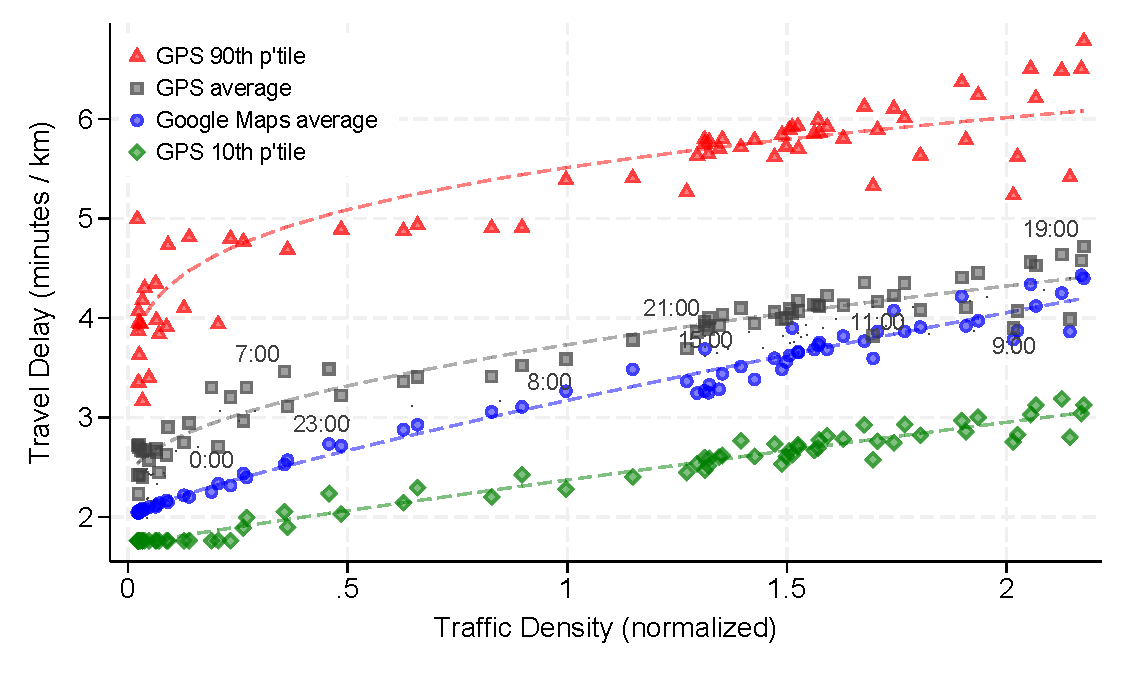
\includegraphics[width=0.5\textwidth]{"figures/smfigure5/panel_A_gps_gm_p10_p90_time.pdf"}
			 & 
			 	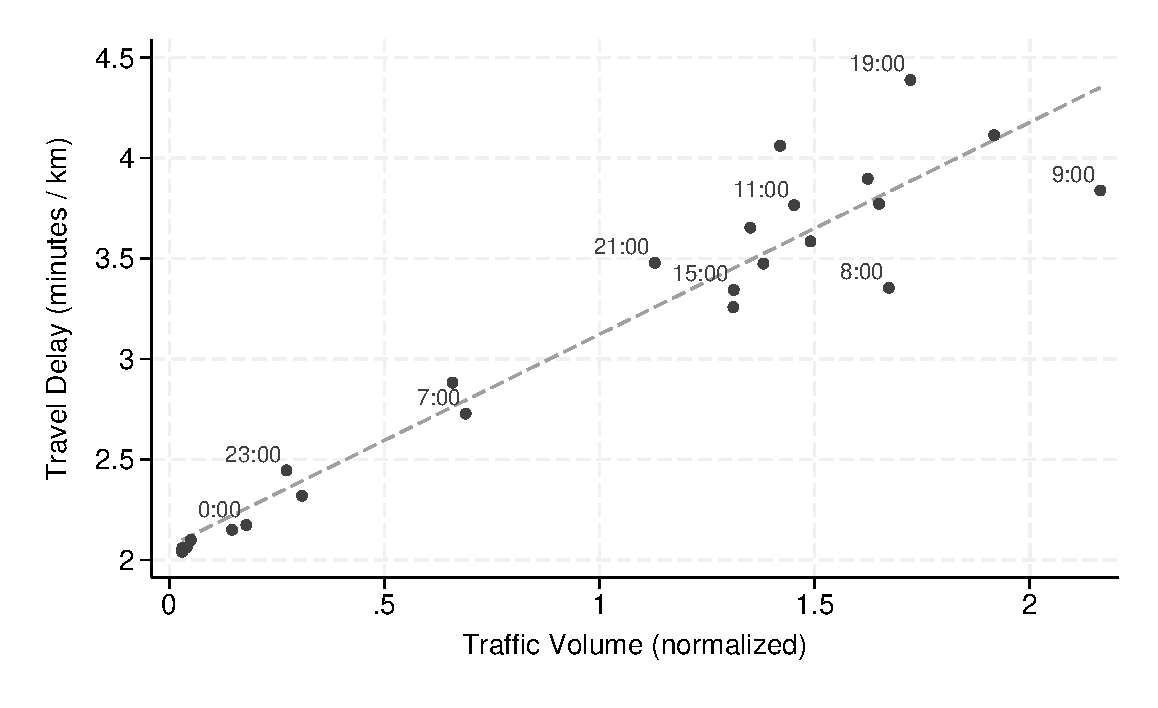
\includegraphics[width=0.5\textwidth]{"figures/smfigure5/panel_B_volume_h.pdf"}
			 \tabularnewline
				{\small{}Panel (A) Travel Delay from GPS Data and Google Maps } & Panel (B) Travel Delay and Traffic Volume
			\tabularnewline
			 & 
			\tabularnewline
				 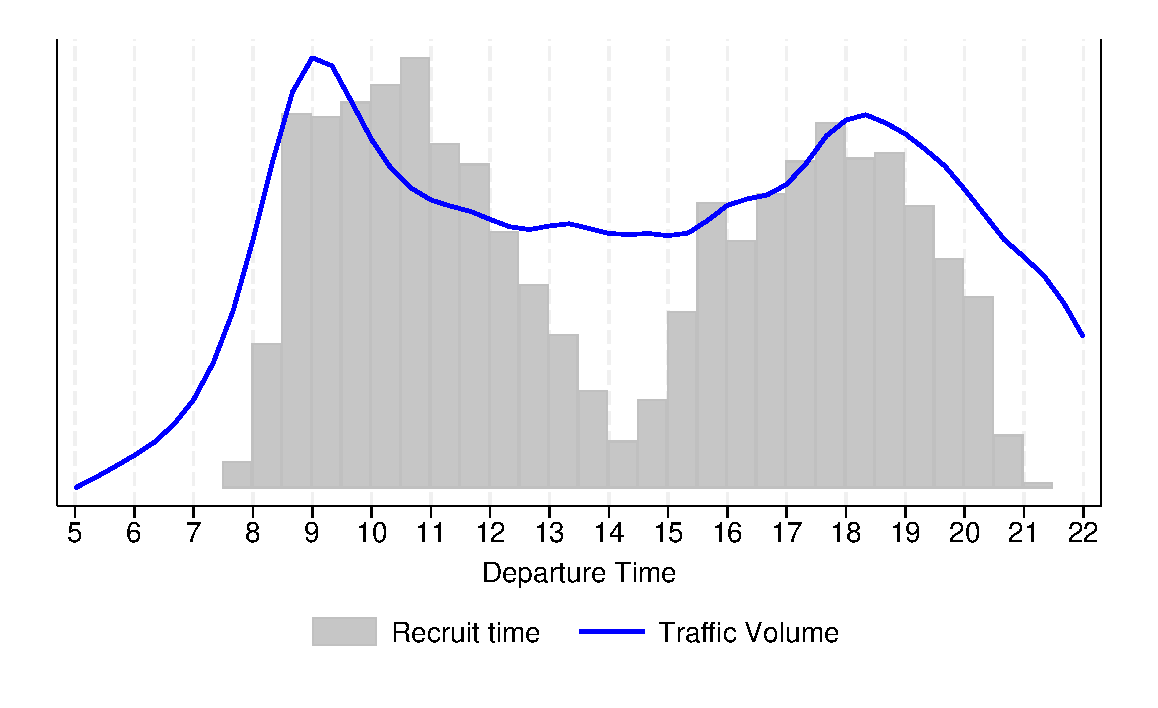
\includegraphics[width=0.5\textwidth]{"figures/smfigure5/panel_C_recruitment.pdf"}
			 & 
				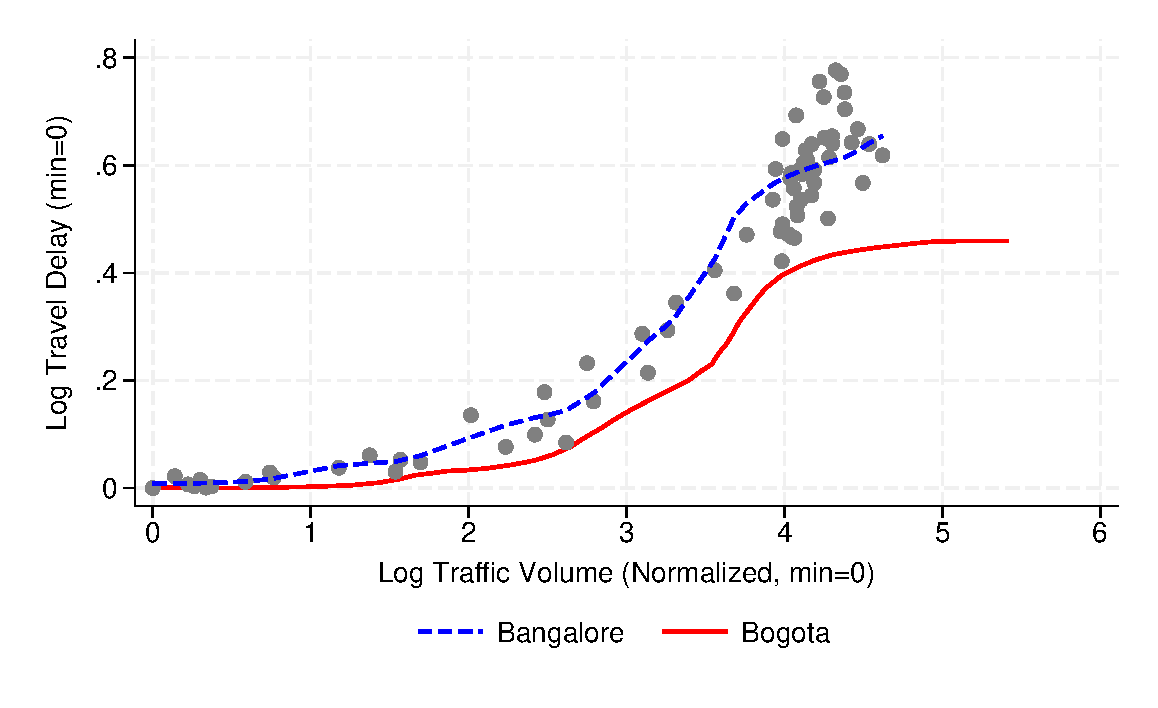
\includegraphics[width=0.5\textwidth]{"figures/smfigure5/panel_D_roadtech_comparison.pdf"}
			\tabularnewline
				Panel (C) Recruitment Time and Trip Time Distributions & Panel (D) Comparison with \citep{duranton2017}
			\tabularnewline
				\includegraphics[width=0.6\textwidth]{"figures/smfigure5/panel_E_two_routes.pdf"} \\
				Panel (E) Peak-hour Use of Lower Externality Routes
			&
				\begin{minipage}[t][0.5\textheight]{0.6\textwidth}
					\vspace{-5cm}
					\small
					Notes: Panel A uses travel delay from GPS trips to replicate Figure \ref{fig:Road-Technology}, including percentiles. The sample is all weekday trips more than 2 kilometers long, without stops along the way, and with a trip diameter to total length ratio above 0.6 (the 25th percentile). For each hour-day I compute the average delay over trips starting in that interval.
					%See notes for Table \ref{tab:Road-Technology-GPS} in \citet{kreindler2023}. 
					Panel B replicates Figure \ref{fig:Road-Technology} with ``volume,'' the normalized number of trips starting each hour on the X axis. Panel C plots the distribution of participant recruitment times (histogram in solid gray) and the distribution of trip departure times (kernel density plot in solid blue line). Both Y axes start at zero. Panel D compares log-log road technology estimates from this paper (gray dots, dashed blue line) with those from \cite{duranton2017} in Bogot{\'a} (red solid line). (Their estimate is computed from Figure 4 panel C.) Panel E describes peak-hour substitution towards routes with less steep travel time profiles. For each commuter in the experimental sample, I query from Google Maps the entire travel time profile for every route that is optimal at some departure time. For each route I compute its slope, the change in travel delay between 6:30 and 9:30 am. The right axis (black dashed line) plots the fraction of commuters for whom their highest slope route is fastest at departure time $h$. The left axis (blue solid line) plots the average slope of the optimal route at $h$.
				\end{minipage}		
		
		\end{tabular}
	}
\par\end{centering}

\end{figure}


\begin{landscape}
\begin{figure}
%\begin{sidewaysfigure}
\caption{Road Technology at the Daily Level \label{fig:road_tech_date}}

\medskip{}

\begin{centering}
%_all_1800
	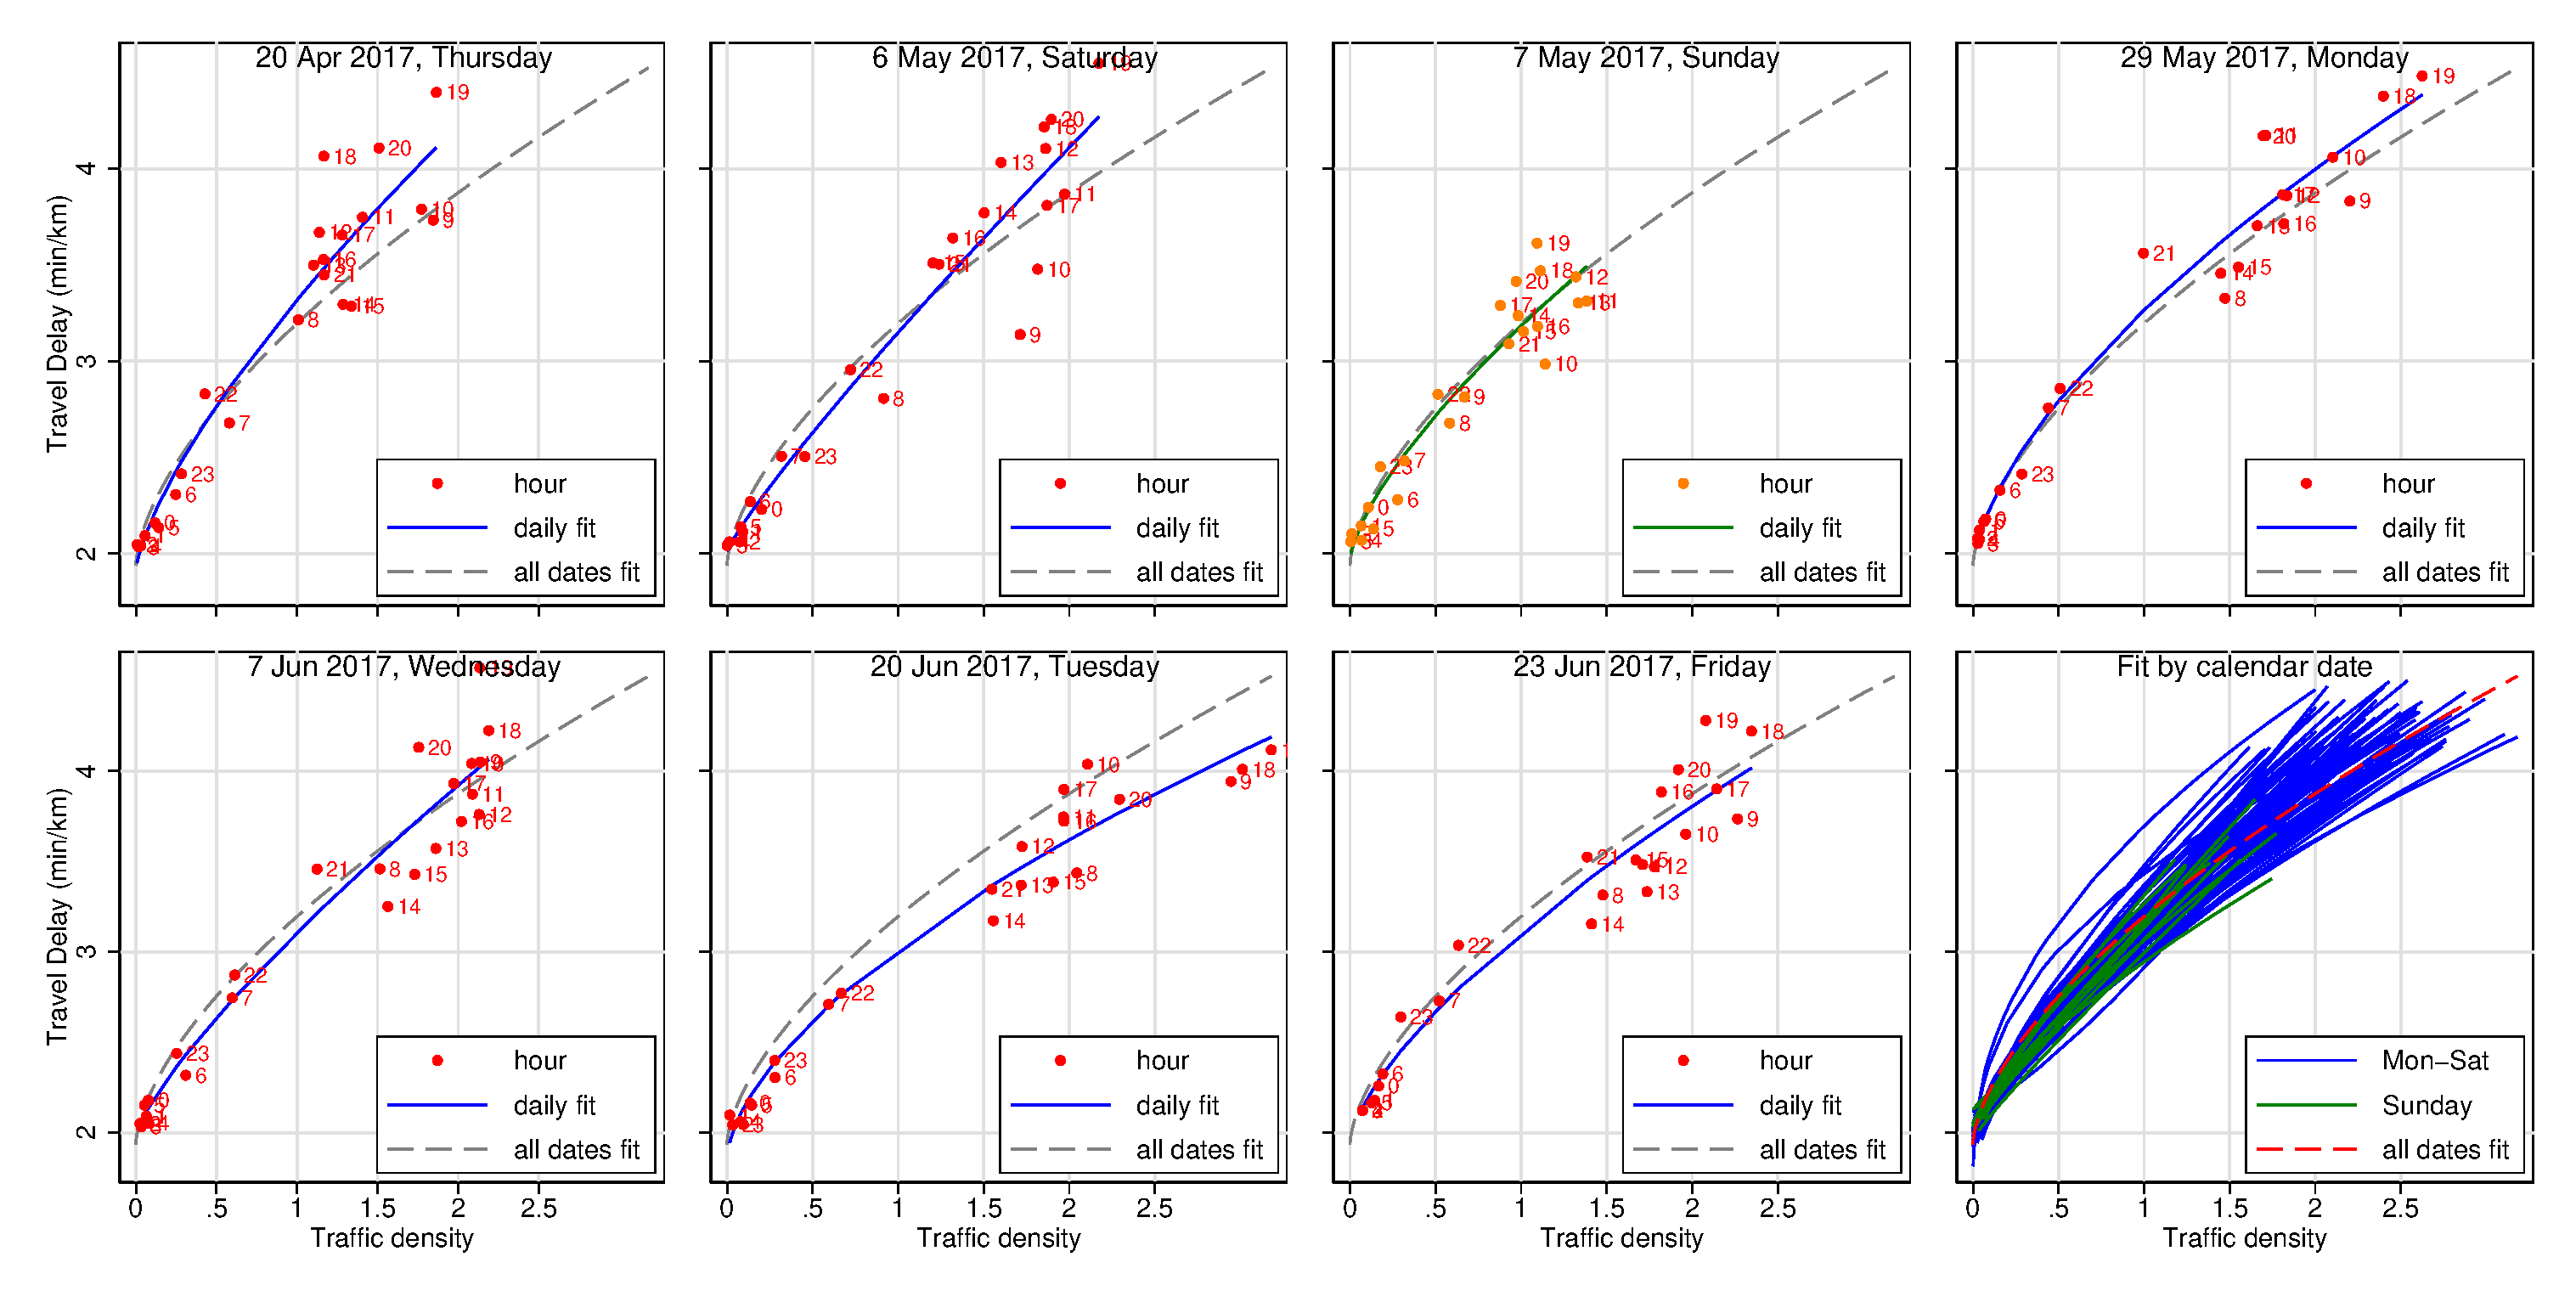
\includegraphics[width=1.5\textwidth]{"figures/smfigure6/combined_all.pdf"}
\par\end{centering}

\medskip{}

{\small{}Notes. These graphs replicate Figure \ref{fig:Road-Technology} panel A by date. The first 7 panels show the relationship between hourly GPS traffic volume and Google Maps travel delay for 7 randomly chosen calendar dates (one for each day of the week). The last panel overlays the predicted fit for all calendar dates in the sample. The sample is calendar dates with above-median number of GPS trips (at least 571 trips per day). Travel delay and traffic density at the day $d$ and hour $h$ level correspond to column 3 in Table \ref{tab:Road-Technology}. Each fit is a power fit as in column 2 in Table \ref{tab:Road-Technology}.\par}
%\end{sidewaysfigure}
\end{figure}
\end{landscape}

\newpage{}

\begin{landscape}
\begin{figure}

\vspace*{-1cm}

\caption{Road Technology on Major Arteries\label{fig:road_tech_artery}}
\begin{centering}
	\includegraphics[width=1.4\textwidth]{"figures/smfigure7/combined_all_density_3600.png"}
\par\end{centering}

{\small{}Notes. These graphs replicate Figure \ref{fig:Road-Technology} for major arteries depicted in \citet{kreindler2023}, Figure A.1., separately by direction. The Y axis is average Google Maps travel delay for that road segment. To compute traffic density at the artery level, I define a buffer area around each artery. I then count the number of GPS trips that travel along the artery in each direction for each time of day, excluding short trips that intersect the artery for less than 200 meters (which I assume correspond to cross-traffic). I obtain 268,292 trip segments on the 46 arteries. 95\% confidence intervals based on Newey-West standard errors with a 3-hour lag also reported.  \par}
\end{figure}
\end{landscape}

\newpage


\begin{figure}[H]
	\vspace{-1cm}		
	\caption{Policy Counterfactual Additional Results\label{fig:sims_additional}}
	\medskip
\begin{centering}
	\makebox[\textwidth][c]{%
		\begin{tabular}{cc}
			
				\includegraphics[width=0.6\textwidth]{"figures/smfigure8/panel_A_so_charges.pdf"}
			& 
				\includegraphics[width=0.6\textwidth]{"figures/smfigure8/panel_B_volumes_nash_so.pdf"}
			\tabularnewline
				Panel (A) Optimal Congestion Charges \vspace{0.25cm} 
			& 
				Panel (B) Departure Volume \vspace{0.25cm}
			\tabularnewline			
				\includegraphics[width=0.6\textwidth]{
				"figures/smfigure8/panel\_C\_density\_power.pdf"}
			& 
				\includegraphics[width=0.6\textwidth]{"figures/smfigure8/panel_D_density_factor.pdf"}
			\tabularnewline
				Panel (C) Non-linear Road Technologies 
			& 
				Panel (D) Varying the Total Volume of Trips	
			\tabularnewline
		\end{tabular}
	}
\par\end{centering}
	\bigskip
	{\small{}Notes. Panel A plots percentiles of the optimal charges (equal to marginal social cost) around the social optimum. For comparison, I plot the average trip delay (red, solid line) as in Figure \ref{fig:Equilibrium-Optimal-Social}, and the instantaneous travel delay (blue, dashed line). Panel B plots the rates of trip departure rates in the Nash equilibrium and in the social optimum. Panel C overlays the alternate road technologies used in panel D of Table \ref{tab:Social-Optimum}, over the benchmark road technology (Figure \ref{fig:Road-Technology}). I use the estimated $\lambda_0$ and $\lambda_1$ from the benchmark linear equation \ref{eq:road-tech} and only vary $\nu$. Panel D shows equilibrium peak average travel delay (X axis) and welfare gain from optimal pricing (Y axis) when varying the total volume of trips used in the simulation. The number near each point is the assumed fraction of all daily trips that happen during peak time. In the benchmark specification, I assume this is 0.2.\par}

\end{figure}


\newpage

\begin{figure}[H]
	\vspace{-1.5cm}		
	\caption{Decomposing Gains and Losses in the Social Optimum\label{fig:sims_decompose}}
	\medskip
	\begin{centering}
		\makebox[\textwidth][c]{%
			\begin{tabular}{cc}	
					\includegraphics[width=0.55\textwidth]{"figures/smfigure9/cost_change_decomposition.pdf"}
				& 
					\includegraphics[width=0.55\textwidth]{"figures/smfigure9/cost_change_decomposition_wcharges.pdf"}
				\tabularnewline
					Panel (A) Real Changes: Travel Time and Schedule Costs 
				& 
					Panel (B) Net of Charges and Rebates
				
			\end{tabular}
		}
		\par\end{centering}
		\bigskip
		{\small{}Notes. For each commuter and ideal arrival time $h_i^A$, the X axis is the average departure time $h_i=\mathbb{E}h(h_i^A)$ in Nash. Panel A plots the Nash--social optimum difference in $-\mathbb{E} \alpha T(h_i)$ vs $h_i$ (black, solid line) and in $-\mathbb{E} \beta_E|h_i+T(h_i)-h_i^A|_{-}+\beta_L|h_i+T(h_i)-h_i^A|_{+}$ vs $h_i$ (green, dashed line). Panel B plots average expected utility change vs $h_i$ when commuters receive a rebate that is proportional to trip length (black, solid line) or constant (green, dashed line).\par}
	
%\end{figure}

%\newpage

%\begin{figure}[H]
%	\vspace{-1cm}
	\caption{Policy Counterfactual in Two Route Equilibrium Model\label{fig:sims_2routes}}
	\medskip
	
	\begin{centering}
		\makebox[\textwidth][c]{%
			\begin{tabular}{cc}
				
					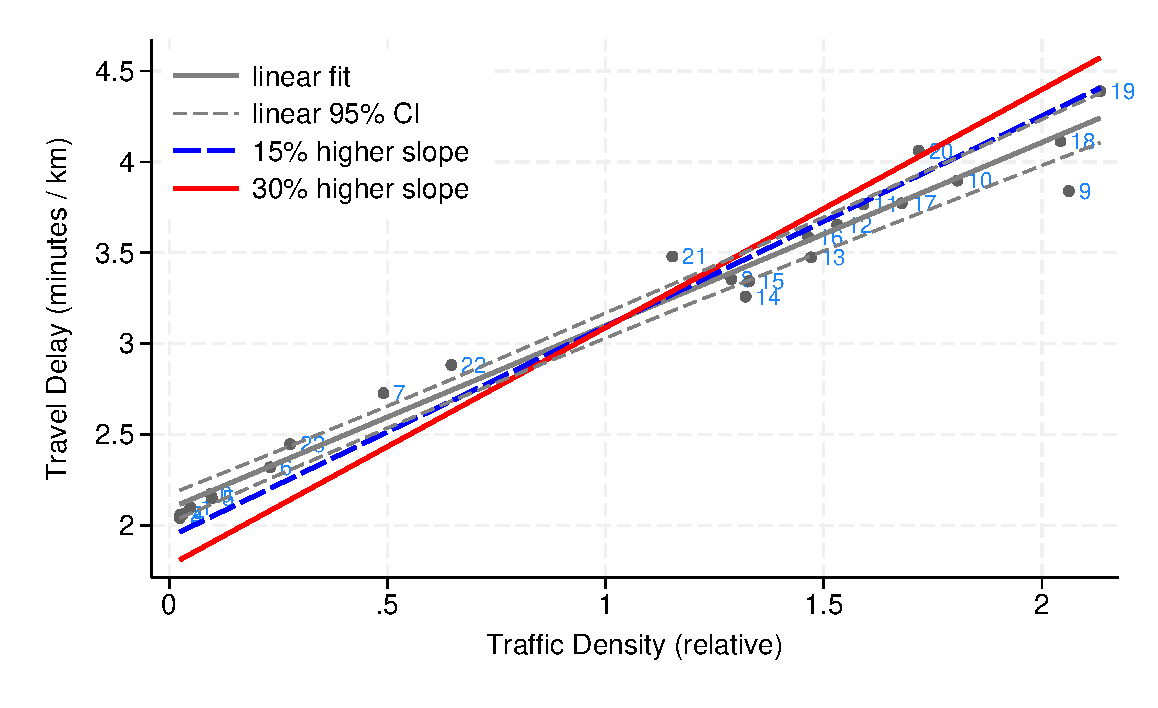
\includegraphics[width=0.55\textwidth]{"figures/smfigure10/panel_A_2routes_road_tech.pdf"}
				& 
					\includegraphics[width=0.55\textwidth]{"figures/smfigure10/2routes_r1_prob.pdf"}
				\tabularnewline
					Panel (A) Road Technology for Two Routes \vspace{0.25cm} 
				& 
					Panel (B) High-Externality Route Choice Prob. \vspace{0.25cm}
				\tabularnewline			
					\includegraphics[width=0.55\textwidth]{"figures/smfigure10/2routes_delays.pdf"} \\
					Panel (C) Average Travel Delay by Route
				& 
				
					\begin{minipage}[t][0.5\textheight]{0.55\textwidth}
						\vspace{-6cm}
						\small
						Notes: This Figure describes the two-route equilibrium (panel E of Table \ref{tab:Social-Optimum}). 				
						Panel A overlays the alternate high-externality route road technologies over the benchmark road technology (Figure \ref{fig:Road-Technology}).
						Panel B plots the probability of taking the high-externality route by departure time, in the Nash equilibrium and in the social optimum, in the two-route model where one route has 15\% higher slope. 
						Panel C replicates Figure \ref{fig:Equilibrium-Optimal-Social} by route for the two-route model where one route has 15\% higher slope.
					\end{minipage}
				
			\end{tabular}
		}
		\par\end{centering}
	%	\bigskip
	%	{\small{}Notes.  \par}
	
\end{figure}


\newpage


\subsection{Supplementary Material: Tables}


\renewcommand{\theHtable}{SM.\Roman{table}} 
\renewcommand{\thetable}{SM.\Roman{table}}
\setcounter{table}{0} 

%\newpage

\begin{table}[H]
\begin{centering}
\caption{Descriptive Statistics about Travel Behavior\label{tab:Descriptive-Statistics-about}}
\par\end{centering}

	\medskip
	\begin{tabular}{lcccccc}
\toprule
\addlinespace\multicolumn{7}{l}{\emph{Panel A. Trip Characteristics}} \\
\ExpandableInput{tables/smtable1/panel_A}
\addlinespace\multicolumn{7}{l}{\emph{Panel B. Commute Destination Variability}} \\
\ExpandableInput{tables/smtable1/panel_B}
\addlinespace\multicolumn{7}{l}{\emph{Panel C. Departure Time Variability}} \\ 
\addlinespace\multicolumn{7}{l}{\emph{(Standard Deviation of the Departure Time in hours)}} \\
\ExpandableInput{tables/smtable1/panel_C}
\bottomrule
\end{tabular}

	\medskip

\begin{singlespace}
{\small Notes: This table reports summary travel behavior statistics for the experimental sample of 497 commuters. See section \ref{sec:GPS-Data} for the definition of home and work locations and of regular commuter. In panel C, I compute the within-commuter variation in departure times for different classes of trips.}{\small \par}
\end{singlespace}
\end{table}





\newpage{}





\begin{table}[H]

\caption{Experimental Design \label{tab:expdesign_matrix}}

\medskip

\begin{centering}
	\textit{Panel A. Treatment Strata} \par
\end{centering}

\medskip

\begin{centering}
	%\resizebox{\textwidth}{!}{
%{
\begin{tabular}{lllllll}
		\toprule

\multicolumn{3}{c}{\textit{\thead{Strata}}}   & \multicolumn{4}{c}{\textit{\thead{Departure Time \\ Sub-treatment}}} \\
      \hline
      % \cline{6-10}      \cline{12-16} \cline{18-20}
\thead{Route \\ Eligibility}  & \thead{Car or \\ Moto} & \thead{Daily KM} & \thead{High \\ Rate} & \thead{Low \\ Rate} & \thead{Info} & \thead{Control} \\
\hline
\addlinespace
Eligible & Car   & Low      & 3/8   & 1/8   & 2/8   & 2/8 \\
Eligible & Car   & High     & 1/8   & 3/8   & 2/8   & 2/8 \\
Eligible & Moto  & Low      & 3/8   & 1/8   & 2/8   & 2/8 \\
Eligible & Moto  & High     & 1/8   & 3/8   & 2/8   & 2/8 \\
\addlinespace
Ineligible & Car   & Low    & 1/12  & 3/12  & 4/12  & 4/12\\
Ineligible & Car   & High   & 3/12  & 1/12  & 4/12  & 4/12\\
Ineligible & Moto  & Low    & 1/12  & 3/12  & 4/12  & 4/12\\
Ineligible & Moto  & High   & 3/12  & 1/12  & 4/12  & 4/12\\
\bottomrule
\end{tabular}
%}
%}
\par
\end{centering}

\medskip
	

\begin{centering}
	\textit{Panel B. Treatment Timing} \par
\end{centering}

\medskip

\begin{centering}
	\begin{tabular}{ccl@{\hskip 0.25in}c@{\hskip 0.25in}c@{\hskip 0.25in}c@{\hskip 0.25in}	c}
\toprule
 % & (1) & (2) & (3) & (4) & (5) & (6) \\
     &                             &                                    & \multicolumn{4}{c}{\thead{ \textit{Treatment by} \\ \textit{Week in Experiment} }  } \\
     \cline{4-7}
\textit{\thead{Route \\ Eligibility}} & \textit{\thead{Dep. Time \\ Timing}} & \textit{\thead{Dep. Time \\ Sub-Treatment} } & 1 & 2 & 3 & 4 \\
\hline
\addlinespace
\multirow{4}{*}{Eligible} & \multirow{4}{*}{Late} & High rate & R & H & H & H \\
						  & 					  & Low  rate & R & L & L & L \\
						  & 					  & Information & R & I & I & I \\
						  & 					  & Control   & R & C & C & C \\
\addlinespace\addlinespace
\multirow{4}{*}{Eligible} & \multirow{4}{*}{Early} & High rate & H & H & H & R \\
						  & 					   & Low  rate & L & L & L & R \\
						  & 					   & Information & I & I & I & R \\
						  & 					   & Control   & C & C & C & R \\
\addlinespace\addlinespace
\multirow{4}{*}{Ineligible} & \multirow{4}{*}{Late} & High rate & I & H & H & H \\
						  & 					  & Low  rate   & I & L & L & L \\
						  & 					  & Information & I & I & I & I \\
						  & 					  & Control   & C & C & C & C \\
\addlinespace\addlinespace
\multirow{4}{*}{Ineligible} & \multirow{4}{*}{Early} & High rate & H & H & H & I \\
						  & 					   & Low  rate & L & L & L & I \\
						  & 					   & Information & I & I & I & I \\
						  & 					   & Control   & C & C & C & C \\
\bottomrule
\end{tabular}
\par
\end{centering}

\medskip

\begin{singlespace}
{\small Notes. There were eight strata in the experiment, all combinations of participants eligible or ineligible for the route charge, car or non-car (motorcycle or scooter) users, and participants with high or low daily travel distance in the baseline period. Departure time sub-treatment probabilities are given in panel A. There are eight route sub-treatments: all combinations of high/low charges, short/long detour, and early/late. All have equal probabilities. Sub-treatment are cross-randomized (see \citealp{kreindler2023}, section A.6.). Treatment timing is presented in panel B. The letter R corresponds to the route treatment. The letters H, L, I and C respectively correspond to high-rate, low-rate, information and control in the departure time treatment.  }
\end{singlespace}

\end{table}






\begin{table}[H]
	\begin{centering}
		\caption{Experimental Participant Sample Representativeness\label{tab:selection_summary}} \par
	\end{centering}

\medskip{}
	
	\begin{centering}
		\resizebox{0.85\textwidth}{!}{
\begin{tabular}{lcccccc}
\toprule
 & (1) & (2) & (3) & (4) & (5) & (6) \\
\addlinespace
 & \multicolumn{2}{c}{In Experiment} & \multicolumn{2}{c}{Not in Experiment} & Difference & \\
\addlinespace
 & Mean & [SD] & Mean & [SD]  &  in SD units & N \\
\addlinespace
\multicolumn{4}{l}{\textit{Panel A. All Respondents Approached}} \\
Male respondent & 0.98 & [0.13]  & 0.97 & [0.17]         & 0.09** &  8,231 \\ 
\addlinespace
Age & 33.3 & [8.2]  & 35.2 & [8.7]         & -0.21*** &  8,231 \\ 
\addlinespace
Car driver & 0.30 & [0.46]  & 0.41 & [0.49]         & -0.24*** &  8,227 \\ 
\addlinespace
Log vehicle price (residual) & 10.5 & [0.4]  & 10.5 & [0.4]         & -0.00 &  7,188 \\ 
\addlinespace\addlinespace
\multicolumn{4}{l}{\textit{Panel B. Survey Respondents}} \\
Log income & 9.96 & [0.71]  & 9.91 & [0.73]         & 0.07 &  2,656 \\ 
\addlinespace
Stated Daily Travel (Km/day) & 47.1 & [24.0]  & 45.1 & [25.1]         & 0.08* &  4,427 \\ 
\addlinespace
Stated Value of Time (Rs/hr) & 206.0 & [138.9]  & 189.0 & [151.3]         & 0.11* &  1,001 \\ 
\addlinespace
Stated Schedule Flexibility (min) & 20.0 & [10.9]  & 18.7 & [12.0]         & 0.11* &    952 \\ 
\bottomrule
\end{tabular}
} \par
	\end{centering}

\medskip{}
\medskip{}
\medskip{}

	\begin{centering}
		\resizebox{\textwidth}{!}{
\begin{tabular}{lcccccccccc}
\toprule
                                             & (1)            & (2)            & (3)            & (4)                & (5)            & (6)            & (7)            & (8)                & (9)            & (10)  \\
                                             & \thead{Business owner\\ or manager}        & \thead{Accountant,\\ Teacher,\\ Doctor}        & \thead{Software\\ and IT}        & \thead{Engineers,\\ Technical}    & \thead{Office\\ staff}        & \thead{Manual\\ jobs}        & \thead{Mobile\\ professions}        & Student    & \thead{Others,\\ Retired}    & Total \\
\addlinespace 
\multicolumn{4}{l}{\textit{Panel C. Survey Respondents}} \\
\addlinespace 
 In Experiment               & 16.7  & 7.5  & 10.3  & 14.3  & 15.4  & 8.4  & 15.6  & 9.0  & 2.9      &   455  \\
 Not in Experiment   & 15.6 & 6.2 & 10.1 & 11.2 & 18.1 & 9.5 & 12.0 & 13.4 & 3.9 & 2,458 \\
\bottomrule
\end{tabular}
} \par
	\end{centering}

	\begin{centering}
		\medskip{}
		\par\end{centering}
	\begin{singlespace}
		{\small{}Notes. These results describe respondent selection into experiment by comparing the experimental sample (497 respondents) to the entire sample of eligible commuters approached in gas stations by the survey team (panel A) and to the full survey sample (panels B and C). The sample in Panel A is all respondents approached in gas stations, excluding ineligible respondents. Weights are used to (a) account for missing data for each variable, and (b) to adjust for the estimated $\sim 52\%$ ineligible respondents among survey refusals (for refusals, $7,218$ respondents did not complete the eligibility filter, and I assume the same proportion were ineligible). Gender, age and car driver variables are visually assessed by the surveyor for all respondents. Vehicle value (residual) is imputed based on vehicle type (car/motorcycle), make and model, using pricing data scrapped from a used-vehicles website in Bangalore, residualized on a ``car'' dummy. Monthly income is self-reported during the recruitment survey (the respondent is handed the tablet to enter the amount confidentially -- the surveyor never sees the amount), truncated at $100,000$ INR ($\sim 1,300$ USD). Occupation is self-reported during the recruitment survey. Value of time and schedule flexibility are based on choices in hypothetical scenarios in a follow-up phone survey; for details, see \citet{kreindler2023}, section A.4.2. The difference in SD units includes significance levels from a (weighted) regression of the row outcome variable on an indicator for being in the experiment. $^{*}p\leq0.10$, $^{**}p\leq0.05$, $^{***}p\leq0.01$}{\small \par}
	\end{singlespace}
\end{table}

\newpage{}



\begin{landscape}
\begin{table}

\caption{Experimental Balance Checks\label{tab:Balance-Table}}

\medskip

\begin{centering}
\resizebox{1.4\textwidth}{!}{
{\begin{tabular}{lc@{\hskip 0.25in}ccc@{\hskip 0.3in}ccc}
\toprule
 & (1) & (2) & (3) & (4) & (5) & (6) & (7)\\
Time of Day & AM \& PM & \multicolumn{3}{c}{AM}     & \multicolumn{3}{c}{PM}  \\
            &          & all & \thead{pre\\ peak} & \thead{post\\ peak} & all & \thead{pre\\ peak} & \thead{post\\ peak} \\
Commuter FE & X & X & X & X & X & X & X \\
\addlinespace\addlinespace\multicolumn{6}{l}{\emph{Panel A. Full Sample}} \\
\ExpandableInput{tables/smtable6/table_panel_A}
\addlinespace\addlinespace\multicolumn{6}{l}{\emph{Panel B. Regular Commuters, Home-Work and Work-Home Trips}} \\
\ExpandableInput{tables/smtable6/table_panel_B}
\addlinespace\addlinespace\multicolumn{6}{l}{\emph{Panel C. Variable Commuters, All Trips}} \\
\ExpandableInput{tables/smtable6/table_panel_C}
\bottomrule
\end{tabular}
}
}
\par\end{centering}

\medskip{}

\begin{singlespace}
{\small{}Notes. This table shows experimental balance checks for the departure time and route treatments. Variables 1,3,4, and 5 are from the recruitment survey, while the remaining eight variables are calculated from the GPS trips data before the experiment. Each row and group of columns combination reports coefficients from a regressions with the row header as outcome. In the ``Route Treatment'' columns, the sample is restricted to 254 participants who receive the route treatment, and the dependent variable is whether the respondent was assigned to the ``early'' route sub-treatment (to receive the route charges in week 1 as opposed to week 4). All regressions include randomization strata dummies. Rows 13 and 14 report the F-statistic and p-value from column-wise joint significance tests. Robust standard errors are shown in parentheses. $^{*}p\leq0.10$, $^{**}p\leq0.05$, $^{***}p\leq0.01$ \par}
\end{singlespace}
%\end{sidewaystable}

\end{table}
\end{landscape}

\newpage{}


\begin{table}[H]
	\vspace{-1cm}
	\caption{GPS Data Quality at Daily Level (Attrition Check)\label{tab:attrition}}
	\medskip
	\begin{centering}
%		\input{tables/AT_balance2/attrition}
		\begin{tabular}{lc@{\hskip 0.25in}ccc@{\hskip 0.3in}ccc}
\toprule
 & (1) & (2) & (3) & (4) & (5) & (6) & (7)\\
Time of Day & AM \& PM & \multicolumn{3}{c}{AM}     & \multicolumn{3}{c}{PM}  \\
            &          & all & \thead{pre\\ peak} & \thead{post\\ peak} & all & \thead{pre\\ peak} & \thead{post\\ peak} \\
Commuter FE & X & X & X & X & X & X & X \\
\addlinespace\addlinespace\multicolumn{6}{l}{\emph{Panel A. Full Sample}} \\
\ExpandableInput{tables/smtable6/table_panel_A}
\addlinespace\addlinespace\multicolumn{6}{l}{\emph{Panel B. Regular Commuters, Home-Work and Work-Home Trips}} \\
\ExpandableInput{tables/smtable6/table_panel_B}
\addlinespace\addlinespace\multicolumn{6}{l}{\emph{Panel C. Variable Commuters, All Trips}} \\
\ExpandableInput{tables/smtable6/table_panel_C}
\bottomrule
\end{tabular}

	\par\end{centering}
	\medskip
	\begin{singlespace}
		{\small{}Notes. This table shows experimental impacts on the quality of the GPS data received from study participants. The outcome is a dummy for good quality GPS data on a given day. The sample covers all non-holiday weekdays for all experiment participants, excluding days outside Bangalore. In the post period, the sample in column 1 is restricted to the departure time treatment period, either the first or the last three weeks. The sample in column 2 is restricted to the first week in the experiment. All specifications include respondent and study cycle fixed effects. Standard errors are clustered at the respondent level. $^{*}p\leq0.10$, $^{**}p\leq0.05$, $^{***}p\leq0.01$}{\small \par}
	\end{singlespace}
\end{table}

%\newpage{}
\vspace{-0.5cm}
\begin{table}[H]
	\begin{centering}
		\caption{Impact of Departure Time Charges on Daily Total Hypothetical Rate: Commuting Trips \label{tab:DT-daily-details}}
		\par\end{centering}
	
	\medskip
	
	\begin{centering}
		\begin{tabular}{lc@{\hskip 0.25in}ccc@{\hskip 0.3in}ccc}
\toprule
 & (1) & (2) & (3) & (4) & (5) & (6) & (7)\\
Time of Day & AM \& PM & \multicolumn{3}{c}{AM}     & \multicolumn{3}{c}{PM}  \\
            &          & all & \thead{pre\\ peak} & \thead{post\\ peak} & all & \thead{pre\\ peak} & \thead{post\\ peak} \\
Commuter FE & X & X & X & X & X & X & X \\
Sample:     & \multicolumn{7}{c}{ \textit{Regular Commuters, Home-Work and Work-Home Trips}} \\
\addlinespace\ExpandableInput{tables/smtable6/table_panel_B}
\bottomrule
\end{tabular}

		\par\end{centering}
	
	\medskip{}
	
	\begin{singlespace}
		{\small Notes: This table reports the impact of departure time charges on daily total hypothetical rates for regular commuters and commuting trips, separately by time interval.
			The sample of users and days, and the specifications, are the same as in Table \ref{tab:DT-daily}, panel B, further restricted to regular commuters and direct trips between their home and work locations (in either direction). Columns (3) and (6) restrict to trips before the peak, i.e. the mid-point of the rate profile. Columns (4) and (7) restrict to trips after the peak. \citet{kreindler2023}, Table A.3., reports these results for variable commuters. Standard errors in parentheses are clustered at the respondent level. $^{*}p\leq0.10$, $^{**}p\leq0.05$, $^{***}p\leq0.01$  \par}
	\end{singlespace}
\end{table}

\newpage{}


\begin{table}[H]
	\begin{centering}
		\caption{Impact of Route Charges on Detour Route Usage\label{tab:A-daily}}
		
		\medskip
		
		\begin{tabular}{lc@{\hskip 0.25in}ccc@{\hskip 0.3in}ccc}
\toprule
 & (1) & (2) & (3) & (4) & (5) & (6) & (7)\\
Time of Day & AM \& PM & \multicolumn{3}{c}{AM}     & \multicolumn{3}{c}{PM}  \\
            &          & all & \thead{pre\\ peak} & \thead{post\\ peak} & all & \thead{pre\\ peak} & \thead{post\\ peak} \\
Commuter FE & X & X & X & X & X & X & X \\
\addlinespace\addlinespace\multicolumn{6}{l}{\emph{Panel A. Full Sample}} \\
\ExpandableInput{tables/smtable6/table_panel_A}
\addlinespace\addlinespace\multicolumn{6}{l}{\emph{Panel B. Regular Commuters, Home-Work and Work-Home Trips}} \\
\ExpandableInput{tables/smtable6/table_panel_B}
\addlinespace\addlinespace\multicolumn{6}{l}{\emph{Panel C. Variable Commuters, All Trips}} \\
\ExpandableInput{tables/smtable6/table_panel_C}
\bottomrule
\end{tabular}

		\par\end{centering}
	
	\medskip
	
	\begin{singlespace}
		{\small{}Notes: This table reports difference-in-differences impacts of the route treatment on trip and daily outcomes. In the first two columns, an observation is a commuting trip between home and work, and the outcome is whether the commuting trip used a detour route (defined as any route that avoids the congestion area). The last two columns, an observation is a commuter, day combination, and the outcome is the total number of trips that day. The sample is all non-holiday weekdays with good quality GPS data, excluding days outside Bangalore. In the post period, all days except trial days are included. The sample is restricted to 243 participants in the route treatment. In the first two columns, only frequent commuters are included. In panel B, the sample is restricted to commuters who used a detour route between home and work at least once before the experiment.	All specifications include respondent and study cycle fixed effects. The mean of the outcome variable in the control (late) group in week 1 of the experiment is reported for each specification. Standard errors in parentheses are clustered at the respondent level. $^{*}p\leq0.10$, $^{**}p\leq0.05$, $^{***}p\leq0.01$}{\small \par}
	\end{singlespace}
\end{table}

\newpage{}


\begin{table}[H]

\caption{Impact of Route Charge Sub-Treatments on Daily Outcomes \label{tab:A-day-subtreats}}
\medskip
\begin{centering}
	{
\def\sym#1{\ifmmode^{#1}\else\(^{#1}\)\fi}
\begin{tabular}{l*{2}{c}}
\toprule
            &\multicolumn{2}{c}{Hypothetical Route Charges}\\\cmidrule(lr){2-3}
            &\multicolumn{1}{c}{(1)}   &\multicolumn{1}{c}{(2)}   \\
\addlinespace\addlinespace
Treated $\times$ High Rate&       -41.1***&               \\
            &      (13.1)   &               \\
\addlinespace
Treated $\times$ Low Rate&       -21.5   &               \\
            &      (13.3)   &               \\
\addlinespace
Treated $\times$ Short Detour&               &       -43.0***\\
            &               &      (15.4)   \\
\addlinespace
Treated $\times$ Long Detour&               &       -26.2   \\
            &               &      (17.8)   \\
\addlinespace\addlinespace
Observations&       6,129   &       3,693   \\
Commuters   &         243   &         148   \\
Control Mean&       117.1   &       122.7   \\
P-val Equal Sub-treatment Effects&        0.30   &        0.48   \\
\bottomrule
\multicolumn{3}{l}{\footnotesize Standard errors in parentheses}\\
\multicolumn{3}{l}{\footnotesize * p$<$.10, ** p$<$.05, *** p$<$.01}\\
\end{tabular}
}

\par\end{centering}

\medskip{}
\medskip{}

\begin{singlespace}
{\small{}Notes: This table reports difference-in-differences impacts of route sub-treatments on daily total hypothetical route charges. The sample in column 1 is the same as in Table \ref{tab:A-daily}, covering the period before and during the first week in the experiment. In column 2 the sample is restricted to 148 route treatment participants for whom candidate areas included at least one with short detour (3-7 minutes) and at least one with long detour (7-14 minutes). The outcome is total daily hypothetical route charges; higher values indicate lower detour usage. Standard errors in parentheses are clustered at the respondent level. $^{*}p\leq0.10$, $^{**}p\leq0.05$, $^{***}p\leq0.01$ \par}
\end{singlespace}
\end{table}


\newpage{}

\begin{table}[H]
	
	\caption{Travel Demand Estimates: Additional Results \label{tab:gmm-other}}
	
	\medskip
	
	\begin{centering}
		\resizebox*{\textwidth}{!}{\begin{tabular}{lcccccc}
   \toprule
   & (1) & (2) & (3) & (4) & (5) & (6) \\
   & \thead{Static \\ Route Choice} & \thead{ Asymmetric \\ switching cost} & Time FE & \thead{ Half \\ attention} & \thead{ Parameters \\ prop. to \\ wage} & \thead{ Single ideal \\ arrival time} \\
   \addlinespace\addlinespace
$\beta_E$: Schedule cost early (INR/hour) & 659 & 569 & 492 & 285 & 418 & 1236 \\ 
    & [436, 1243] & [341, 1860] & [271, 1838] & [196, 1184] & [197, 3441] & [422, 47640] \\ 
   \addlinespace
$\beta_L$: Schedule cost late (INR/hour) & 521 & 409 & 366 & 286 & 603 & 645 \\ 
    & [262, 1827] & [228, 1293] & [253, 1833] & [151, 943] & [209, 1733] & [90, 1133] \\ 
   \addlinespace
$\alpha$: Value of travel time (INR/hour) & 2199 & 1480 & 543 & 327 & 398 & 727 \\ 
    & [1634, 2383] & [716, 2617] & [83, 1632] & [148, 713] & [119, 1047] & [345, 1479] \\ 
   \addlinespace
$\gamma$: Route switching cost (INR) &  & 16.8 & 104.9 & 52.3 & 83.1 & 74.6 \\ 
    &  & [0.0, 44.0] & [39.2, 158.4] & [27.9, 72.6] & [29.2, 115.4] & [30.0, 92.5] \\ 
   \addlinespace
$\sigma^{DT}$: Logit departure time & 19.2 & 19.6 & 21.2 & 14.7 & 33.2 & 106.9 \\ 
    & [1.0, 104.4] & [1.0, 112.5] & [1.3, 101.0] & [1.0, 104.5] & [1.7, 346.6] & [3.5, 547.0] \\ 
   \addlinespace
$\sigma^R$: Logit route nest & 95.8 & 69.3 & 57.7 & 33.6 & 46.1 & 59.7 \\ 
    & [60.1, 115.2] & [31.1, 87.8] & [27.2, 81.8] & [23.4, 43.4] & [24.5, 68.7] & [36.4, 71.0] \\ 
   \addlinespace
\addlinespace 
\multicolumn{7}{l}{\textit{Model Components:}}  \\ 
 \addlinespace 
  Route choice model           & Static & Dynamic & Dynamic  & Dynamic & Dynamic  & Dynamic \\ 
 \addlinespace 
  Fixed discount factor ($\delta$)  & - & 0.90 & 0.90 & 0.90 & 0.90 & 0.90 \\ 
 \addlinespace 
  Asymmetric switch cost ($\gamma_{01}=2\gamma_{10}$)  & - & Yes &  -  &  -  &  -  &  -  \\ 
 \addlinespace 
  Route Choice Time FE                 & - & -   & Yes &  -  &  -  &  -  \\ 
 \addlinespace 
 \addlinespace 
\multicolumn{7}{l}{\textit{Moments:}}  \\ 
 \addlinespace 
  Departure Time (49)           & Yes & Yes & Yes & Yes & Yes & Yes  \\ 
 \addlinespace 
  Dynamic route choice (10)     & -   & Yes & Yes & Yes & Yes & Yes\\ 
 \addlinespace 
  Static route choice (2)       & Yes & -   & -   & -   & -   & -  \\ 
 \addlinespace 
    \bottomrule 
 \end{tabular} 
 } 


	\par\end{centering}
	
	\medskip{}
	
	\begin{singlespace}
		{\small Notes: Column 1 fits a model with static route choice ($\delta=\gamma=0$) using only two route choice moments: the fraction using route 1 when not charged during the experiment, and when charged. Column 2 modifies the benchmark model to include asymmetric switching costs parametrized by $\gamma_{01}=\gamma_{10}=2\gamma$. Column 3 estimates time fixed effects $\eta_1,\eta_2, \eta_3,\eta_4$ that enter route 1 utility on the corresponding weeks during the experiment. Column 4 imposes that each commuter ignores experimental congestion charges with independent probability $p=0.5$. In column 5, all preference parameters are proportional to $w_i$, commuter $i$'s self-reported hourly wage. (Note that logit parameters are proportional to $w_i$ and to normalized trip length, i.e. $\sigma^{DT}_i=\sigma \frac{w_i}{\overline w}\frac{K_i}{\overline K}$). In column 6, I assume that all commuters have the same ideal arrival time that does not vary over time, $h_{it}^A=h^A$. \par}
	\end{singlespace}
\end{table}

\newpage{}

\begin{table}[H]
	
	\caption{Travel Demand Estimation: Discount Factor Robustness \label{tab:gmm-delta}}
	\medskip
	\begin{centering}
		\resizebox*{\textwidth}{!}{\begin{tabular}{lccccc}
   \toprule
   & (1) & (2) & (3) & (4) & (5) \\
 \addlinespace 
   & \multicolumn{4}{c}{Varying Discount Factor $\delta$} & Estimate $\delta$  \\
   \addlinespace\addlinespace
$\beta_E$: Schedule cost early (INR/hour) & 570 & 506 & 545 & 561 & 548 \\ 
    & [333, 1694] & [276, 1184] & [312, 1821] & [313, 1517] & [297, 2032] \\ 
   \addlinespace
$\beta_L$: Schedule cost late (INR/hour) & 381 & 365 & 348 & 354 & 350 \\ 
    & [227, 1074] & [243, 1549] & [248, 1234] & [235, 1226] & [237, 1091] \\ 
   \addlinespace
$\alpha$: Value of travel time (INR/hour) & 1180 & 712 & 611 & 593 & 623 \\ 
    & [588, 1537] & [285, 1300] & [340, 1279] & [404, 1229] & [250, 1080] \\ 
   \addlinespace
$\gamma$: Route switching cost (INR) & 78.5 & 89.2 & 80.1 & 87.0 & 79.9 \\ 
    & [46.5, 107.6] & [56.8, 128.8] & [37.4, 110.0] & [40.1, 101.8] & [61.7, 117.8] \\ 
   \addlinespace
$\sigma^{DT}$: Logit departure time & 22.6 & 21.1 & 20.5 & 20.7 & 20.5 \\ 
    & [1.0, 112.9] & [1.9, 72.2] & [1.0, 70.3] & [1.0, 91.3] & [1.4, 83.9] \\ 
   \addlinespace
$\sigma^R$: Logit route (upper nest) & 62.0 & 57.7 & 57.9 & 50.6 & 58.6 \\ 
    & [31.6, 63.5] & [37.3, 66.2] & [41.6, 74.9] & [34.0, 67.2] & [39.3, 69.2] \\ 
   \addlinespace
$\delta$: discount factor & 0.00 & 0.50 & 0.90 & 0.99 & 0.88 \\ 
    &  &  &  &  & [0.37, 0.99] \\ 
   \addlinespace
\addlinespace 
\multicolumn{6}{l}{\textit{Model:}}  \\ 
 \addlinespace 
  Dynamic route choice model           & Dynamic & Dynamic  & Dynamic  & Dynamic  & Dynamic \\ 
 \addlinespace 
  Fixed discount factor ($\delta$)  & 0.0 & 0.50 & 0.90 & 0.99 &  -  \\ 
 \addlinespace 
 \addlinespace  
\multicolumn{6}{l}{\textit{Moments:}}  \\ 
 \addlinespace 
  Dynamic route choice (10)     & Yes & Yes & Yes & Yes & Yes \\ 
 \addlinespace 
  Route choice transition (1)   & -   &  -  &  -  &  -  & Yes \\ 
 \addlinespace 
    \bottomrule 
 \end{tabular} 
 } 


	\par\end{centering}	
	\medskip{}
	\begin{singlespace}
		{\small Notes: Columns 1-4 replicate column 1 in Table \ref{tab:gmm} with different assumptions on $\delta$. In column 5 I estimate $\delta$, using an additional moment. This moment measures the transition probability between route 0 and route 1, on average, between weeks 1-2, 2-3, and 3-4 during the experiment. In the data, I define that the commuter uses route 0 if the average weekly route choice of route 0 is strictly below $0.5$. \par}
	\end{singlespace}
\end{table}

\newpage{}

\begin{table}
	\caption{Dynamic Route Choice Model Identification{\label{tab:gmm-vott-jacobian}}}
	
	\medskip
	
	\begin{centering}
			\resizebox*{\textwidth}{!}{
				\resizebox*{\textwidth}{!}{\begin{tabular}{lccc@{\hskip 1cm}ccc@{\hskip 1cm}ccc}
   \toprule
   & \multicolumn{3}{c}{(1)} & \multicolumn{3}{c}{(2)} & \multicolumn{3}{c}{(3)}  \\ 
   \addlinespace
   & \multicolumn{3}{c}{Full Model} & \multicolumn{3}{c}{No departure time} & \multicolumn{3}{c}{Simple Model ($\delta=0$)} \\ 
   \addlinespace
   & $\alpha$ & $\sigma^R$ & $\sigma^R$   & $\alpha$ & $\gamma$ & $\sigma^R$   & $\alpha$ & $\gamma$ & $\sigma^R$ \\ 
   \addlinespace
 Estimated values  & 611.2 & 80.1 & 57.9 & 561.7 & 86.4 & 57.6 & 808.8 & 98.9 & 62.8  \\ 
   \addlinespace\addlinespace
 \multicolumn{10}{l}{\textit{Jacobian: Change in Route 1 take-up Due to Change in Parameter}}  \\ 
   \addlinespace
 Before Experiment & -0.1 & -0.09 & 0.24 & -0.08 & -0.09 & 0.26 & -0.19 & -0.06 & 0.24 \\ 
 \addlinespace
 Week 1 (Charges) & -0.24 & -0.39 & 0.22 & -0.26 & -0.41 & 0.26 & -0.4 & -0.35 & 0.25 \\ 
 \addlinespace
 Week 2 (After Charges) & -0.19 & -0.12 & 0.29 & -0.22 & -0.14 & 0.31 & -0.38 & -0.06 & 0.19 \\ 
 \addlinespace
   \bottomrule 
 \end{tabular} 
 } 


			}
	\par\end{centering}
	
	\medskip{}

	\begin{singlespace}
		{\small{}Notes: This table reports the Jacobian matrix for three moments with respect to three route choice parameters (VOTT $\alpha$, switch cost $\gamma$ and logit scale $\sigma^R$). The three moments are the route treatment ``early'' group average detour route usage (1) before the experiment, (2) during week 1 in the experiment (when charges were in effect), and (3) in week 2 (after charges had ended). The first group of columns uses the benchmark model, and the next group uses the dynamic route choice model without departure time (column 4 in Table \ref{tab:gmm}). In the last group of columns, I estimate a simple model where a single agent faces the average detour (6.4 minutes) and the average route charge (144 INR), and I assume $\delta=0$ (see Supplementary Material \ref{app:vott-id}). Jacobian entries are divided by the value of the parameter, so they represent the semi-elasticity of the moment with respect to a proportional change in the parameter.		
		\par}
	\end{singlespace}
\end{table}
%\newpage{}
\begin{table}[H]
	\caption{Travel Demand Model Finite Sample Properties Check\textbf{\label{tab:gmm-numerical-identification}}}
	
	\medskip
	
	\begin{centering}
	%	\input{tables/T_GMM/GMM_id}
		\begin{tabular}{lc@{\hskip 0.25in}ccc@{\hskip 0.3in}ccc}
\toprule
 & (1) & (2) & (3) & (4) & (5) & (6) & (7)\\
Time of Day & AM \& PM & \multicolumn{3}{c}{AM}     & \multicolumn{3}{c}{PM}  \\
            &          & all & \thead{pre\\ peak} & \thead{post\\ peak} & all & \thead{pre\\ peak} & \thead{post\\ peak} \\
Commuter FE & X & X & X & X & X & X & X \\
\addlinespace\addlinespace\multicolumn{6}{l}{\emph{Panel A. Full Sample}} \\
\ExpandableInput{tables/smtable6/table_panel_A}
\addlinespace\addlinespace\multicolumn{6}{l}{\emph{Panel B. Regular Commuters, Home-Work and Work-Home Trips}} \\
\ExpandableInput{tables/smtable6/table_panel_B}
\addlinespace\addlinespace\multicolumn{6}{l}{\emph{Panel C. Variable Commuters, All Trips}} \\
\ExpandableInput{tables/smtable6/table_panel_C}
\bottomrule
\end{tabular}

		\medskip{}
		\par\end{centering}
	\begin{singlespace}
		{\small{}Notes: This table uses simulated data of exactly the same size as the data used in estimation to describe the finite sample properties of the estimation procedure. See notes for Figure \ref{fig:gmm-numerical-identification}. Each column reports results from a quantile (median) regression of the estimated parameter on the vector of true parameters. $^{*}p\leq0.10$, $^{**}p\leq0.05$, $^{***}p\leq0.01$}{\small \par}
	\end{singlespace}
\end{table}

\end{appendices}



\end{document}
